\documentclass[10pt, letterpaper]{report}
% !TeX program = xelatex
%==================PREAMBOLO=======================%
\usepackage[utf8]{inputenc}
\usepackage{psvectorian}
\usepackage{pgfplots}
\usepackage[Rejne]{fncychap}
\usepackage[export]{adjustbox}
\usepackage[T1]{fontenc}
\usepackage{lmodern}
\usepackage[shortlabels]{enumitem}
\usepackage{moresize}
\usepackage{graphicx} % Required for inserting images
\usepackage{hyperref}
\usepackage{listings}
\usepackage[table,xcdraw]{xcolor}
\usepackage{amssymb}
\usepackage{amsmath}
\usepackage[italian]{babel}
\usepackage{nicefrac, xfrac}
\usepackage{tikz}
\usepackage{mathrsfs} 
\usepackage{titletoc}
\usepackage{fancyhdr}
\usepackage{psvectorian,lipsum}
\usepackage{fourier-orns}
\usepackage{lipsum}
\usepackage[paper=a4paper,left=25mm,right=25mm,bottom=25mm,top=25mm]{geometry}
\definecolor{light-gray}{gray}{0.95}
\definecolor{cop}{HTML}{f7ecd7}
\definecolor{copAut}{HTML}{ababab}
\definecolor{copAut2}{HTML}{c3c3e6}
\definecolor{purcop}{HTML}{d0d3db}
\definecolor{sapienza}{HTML}{660f1d}
\definecolor{lightSapienza}{HTML}{e3d3d5}
\definecolor{darkgreen}{HTML}{008000}
\definecolor{cartaRiciclata}{HTML}{fcfcf7}
\newcommand{\redText}[1]{\color{red}#1\color{black}}
\newcommand{\code}[1]{\colorbox{light-gray}{\texttt{#1}}}
\newcommand{\codee}[1]{\colorbox{white}{\texttt{#1}}}
\newcommand{\K}{{\mathbb K}}
\newcommand{\notimplies}{%
  \mathrel{{\ooalign{\hidewidth$\not\phantom{=}$\hidewidth\cr$\implies$}}}}
\newcommand{\flowerLine}{ \begin{center}\decofourleft\hphantom{ }\decoone\hphantom{ }\decofourright\hphantom{}\hphantom{aa}
\decofourleft\hphantom{ }\decoone\hphantom{ }\decofourright\hphantom{}\hphantom{aa}
\decofourleft\hphantom{ }\decoone\hphantom{ }\decofourright\hphantom{}\hphantom{aa}
\decofourleft\hphantom{ }\decoone\hphantom{ }\decofourright\hphantom{}\hphantom{aa} 
\decofourleft\hphantom{ }\decoone\hphantom{ }\decofourright\hphantom{}\hphantom{aa}
\decofourleft\hphantom{ }\decoone\hphantom{ }\decofourright\hphantom{}\hphantom{aa}
\decofourleft\hphantom{ }\decoone\hphantom{ }\decofourright\hphantom{}\hphantom{aa}
\decofourleft\hphantom{ }\decoone\hphantom{ }\decofourright\hphantom{}\hphantom{aa}
\decofourleft\hphantom{ }\decoone\hphantom{ }\decofourright\hphantom{}\hphantom{aa}
\end{center}}
\definecolor{g}{RGB}{60, 50, 50}
\newcommand{\textg}[1]{\color{g}{\textbf{#1}}\color{black}}
\newcommand{\teo}[1]{{\large\color{sapienza}\textbf{Teorema #1 :\hphantom{a}}}}
\newcommand{\defi}[1]{{\large\color{sapienza}\textbf{Definizione #1 :\hphantom{a}}}}
\newcommand{\claim}[1]{{\color{sapienza}\textbf{Claim #1 :\hphantom{a}}}}
\newcommand{\lemma}[1]{{\color{sapienza}\textbf{Lemma #1 :\hphantom{a}}}}
\newcommand{\dimo}[1]{{\color{sapienza}\textbf{Dimostrazione #1 :\hphantom{a}}}}
\newcommand{\prop}[1]{{\color{sapienza}\textbf{Proposizione #1 :\hphantom{a}}}}
\newcommand\greybox[1]{%
  \vskip\baselineskip%
  \par\noindent\colorbox{light-gray}{%
    \begin{minipage}{\textwidth}#1\end{minipage}%
  }%
  \vskip\baselineskip%
}
\newcommand\sapbox[1]{%
  \vskip\baselineskip%
  \par\noindent\colorbox{lightSapienza}{%
    \begin{minipage}{\textwidth}#1\end{minipage}%
  }%
  \vskip\baselineskip%
}

\newcommand{\Z}{{\mathbb Z}}
\newcommand{\blank}{{\sqcup}}
\newcommand{\R}{{\mathbb R}}
\newcommand{\N}{{\mathbb N}}
\newcommand{\C}{{\mathbb C}}
\newcommand{\Sn}{{\mathcal S_n}}
\newcommand{\An}{{\mathcal A_n}}
\newcommand{\E}{{\mathcal E}}
\newcommand{\B}{{\mathcal B}}
\newcommand{\mcm}{{\text{mcm}}}
\newcommand{\rg}{{\text{rg}}}
\newcommand{\ve}{{\bar v}}
\newcommand{\spaz}{{\text{\hphantom{aa}}}}
\newcommand{\MCD}{{\text{MCD}}}
\newcommand{\tc}{{\text{ tale che }}}
\newcommand{\supp}{{\text{Supp}}}
\newcommand{\acc}{\\\hphantom{}\\}
\newcommand{\aut}{{\text{Aut}}}
\newcommand{\Span}{{\text{Span}}}
\newcommand{\End}{{\text{End}}}
\newcommand{\cen}{{\text{Centro}}}
\newcommand{\norm}{{\unlhd}}
\newcommand{\ciclS}{{\left \langle }}
\newcommand{\ciclE}{{\right \rangle }}
\newcommand{\boxedMath}[1]{\begin{tabular}{|c|}\hline \texttt{#1} \\ \hline\end{tabular} :}
\newcommand{\shell}[1]{\colorbox{black}{\textcolor{white}{\texttt{#1}}}}
\newcommand{\eqImportante}[1]{\begin{center}\huge\lefthand\hphantom{a}
    \normalsize\texttt{#1}
    \hphantom{aaa}\huge\righthand\end{center}}

\fancyhf{}
\pagestyle{fancy}
\usepackage{pgf-pie}  
\usetikzlibrary{positioning}

\renewcommand{\headrule}{%
\vspace{-8pt}\hrulefill
\raisebox{-2.1pt}{\quad\decothreeleft\decotwo\decothreeright\quad}\hrulefill}

%sta roba serve per il codice C
\definecolor{mGreen}{rgb}{0,0.6,0}
\definecolor{mGray}{rgb}{0.5,0.5,0.5}
\definecolor{mPurple}{rgb}{0.58,0,0.82}
\definecolor{backgroundColour}{rgb}{0.95,0.95,0.92}

\lstdefinestyle{CStyle}{
    backgroundcolor=\color{backgroundColour},   
    commentstyle=\color{mGreen},
    keywordstyle=\color{magenta},
    numberstyle=\tiny\color{mGray},
    stringstyle=\color{mPurple},
    basicstyle=\footnotesize,
    breakatwhitespace=false,         
    breaklines=true,                 
    captionpos=b,                    
    keepspaces=true,                 
    numbers=left,                    
    numbersep=5pt,                  
    showspaces=false,                
    showstringspaces=false,
    showtabs=false,                  
    tabsize=2,
    language=C
}
\lstdefinestyle{CppStyle}{
    backgroundcolor=\color{backgroundColour},   
    commentstyle=\color{mGreen}\ttfamily,
    morecomment=[l][\color{magenta}]{\#}
    keywordstyle=\color{blue}\ttfamily,
    numberstyle=\tiny\color{mGray},
    stringstyle=\color{red}\ttfamily,
    basicstyle=\ttfamily,
    breakatwhitespace=false,         
    breaklines=true,                 
    captionpos=b,                    
    keepspaces=true,                 
    numbers=left,                    
    numbersep=5pt,                  
    showspaces=false,                
    showstringspaces=false,
    showtabs=false,                  
    tabsize=2,
    language=C
}
\lstset{language=C++,
                basicstyle=\ttfamily,
                keywordstyle=\color{blue}\ttfamily,
                stringstyle=\color{red}\ttfamily,
                commentstyle=\color{green}\ttfamily,
                morecomment=[l][\color{magenta}]{\#}
}
%fine roba che serve per il codice C
\usepackage{minted}
 %TOGLI COMMENTO SE USI XELATEX
%\usepackage{fontspec}
\title{Programmazione di Sistemi Multicore} %========TITOLO========%
\author{Marco Casu}
\date{\vspace{-5ex}}
\begin{document}

%==================COPERTINA=======================%
\begin{titlepage}
    \pagecolor{purcop}
\begin{center}
    %TOGLI COMMENTO SE USI XELATEX
   %\setmainfont{Palace Script MT}
   \Huge Marco Casu\acc
    %\setmainfont{Grand Casino}
     %TOGLI COMMENTO SE USI XELATEX
    %\setmainfont{h Halfroad}
    \HUGE \decothreeleft\hphantom{ }{\Huge\selectfont Programmazione di Sistemi Multicore}\hphantom{ }\decothreeright
     %TOGLI COMMENTO SE USI XELATEX
   % \setmainfont{Times New Roman}
\end{center}
\thispagestyle{empty}
\begin{figure}[h]
    \centering{
        %l'immagine deve avere una risoluzione 2048x2048
        
\includegraphics[width=1\textwidth ]{images/copertina.jpeg}
    }
\end{figure}
\vfill 
\centering 
\includegraphics[width=0.4\textwidth ]{../../../preamble/Stemma_sapienza.png} \acc
\centering \Large \color{sapienza}Facoltà di Ingegneria dell'Informazione,
Informatica e Statistica\\
Dipartimento di Informatica
\end{titlepage}

%===================FINE COPERTINA======================%
\newpage
\pagecolor{cartaRiciclata}%\setmainfont{Algerian}
\large
Questo documento è distribuito sotto la licenza 
\color{blue}\href{https://www.gnu.org/licenses/fdl-1.3.txt}{GNU}\color{black},  
è un resoconto degli appunti (eventualmente integrati con libri di testo) tratti dalle lezioni del corso di Programmazione di Sistemi Multicore
\hphantom{a}per la laurea 
triennale in Informatica. Se dovessi notare errori, ti prego di segnalarmeli.
\vfill
\begin{figure}[h!]
    \raggedright
    
\includegraphics[width=0.4\textwidth,right ]{../../../preamble/tomodachi.pdf} 
\end{figure}
\newpage %\setmainfont{Times New Roman}
\normalsize
\tableofcontents 
\newpage

%==================FOOTER e HEADER=======================%
\fancyhf{}
\fancyhead[L]{\nouppercase{\leftmark}}
\fancyhead[R]{Sezione \thesection}
\fancyfoot[C]{\thepage}
\fancyfoot[L]{Appunti di Prog. di Sistemi Multicore}
\fancyfoot[R]{ Marco Casu}
%\fancyfoot[R]{\setmainfont{Palace Script MT}\huge Marco Casu \setmainfont{Times New Roman}}
%==================FOOTER e HEADER=======================%

%Ricorda del comando \flowerLine per separare le sottosezioni. Le sezioni si separano nelle diverse pagine

%==================INIZIO======================%

\chapter{Parallelismo : Motivazioni}
\section{Introduzione}
In una \textit{GPU} (Graphics Processing Unit), nota anche come scheda video, ci sono circa 
80 miliardi di transistor, e vengono utilizzate per allenare i grossi modelli di intelligenza 
artificiale, i quali necessitano migliaia di GPU, non è un caso se \textit{Nvidia} ad oggi, con 
il boom dell'IA, è una delle aziende più quotate al mondo. Le GPU, e la loro 
programmazione, sono uno fra i principali argomenti di questo corso.\acc 
L'evoluzione dell'hardware, ha portato i grossi sistemi di computazione, ad essere formati da 
svariate unità di calcolo piuttosto che una singola unità molto potente, i processori stessi di uso comune, 
ad oggi sono composti da più \textit{core}.\acc 
La legge di Moore riguarda una stima empirica che mette in correlazione lo scorrere del tempo con 
l'aumentare della potenza di calcolo dei processori, se inizialmente, a partire dagli anni 70, tale potenza 
raddoppiava ogni due anni, ad oggi tale andamento è andato rallentando, raggiungendo un 
incremento 1.5 in 10 anni.
\begin{center}
    \includegraphics[width=300pt]{images/processor_trend.eps}
\end{center}
L'obbiettivo di costruire calcolatori sempre più potenti è dipeso dalla necessità dell'Uomo 
di risolvere problemi sempre più complessi, come ad esempio, la risoluzione del genoma umano.\acc 
Il motivo per il quale non è possibile costruire processori monolitici sempre più potenti, risiede 
in un \textit{limite fisico} riguardante la densità massima possibile dei transistor in 
un chip.\begin{enumerate}
    \item transistor più piccoli $\longrightarrow$ processori più veloci
    \item processori più veloci $\longrightarrow$ aumento del consumo energetico 
    \item aumento del consumo energetico $\longrightarrow$ aumento del calore 
    \item aumento del calore $\longrightarrow$ problemi di inaffidabilità dei transistor
\end{enumerate}
\flowerLine
\section{Modelli di Parallelismo}
L'informatico che intende scrivere del codice per un sistema multicore, deve esplicitamente 
sfruttare i diversi core, limitandosi a scrivere un codice sequenziale, non starebbe sfruttando a pieno 
l'hardware a disposizione, rendendo il processo meno efficiente di quanto potrebbe essere.\acc 
La maggior parte delle volte, un algoritmo sequenziale, non può essere direttamente tradotto in un 
algoritmo parallelo, per questo bisogna scrivere il codice facendo riferimento all'hardware di 
destinazione. Si consideri adesso il seguente codice sequenziale, che ha lo scopo di sommare 
$n$ numeri dati in input.
\begin{lstlisting}[style=CStyle]
    sum = 0;
    for(i=0; i<n; i++){
        x = compute_next_value(...);
        sum += x;
    }
\end{lstlisting}
Si vuole rendere tale algoritmo parallelo, sapendo di essere a disposizione di $p$ core.
\begin{lstlisting}[style=CStyle]
    local_sum = 0;
    first_index = ...;
    last_index = ...;
    for(local_i=first_index; first_index<last_index; local_i++){
        local_x = compute_next_value(...);
        local_sum += local_x;
    }
\end{lstlisting}
In tale esempio, ogni core possiede le sue variabili private non condivise con gli altri core, 
ed esegue indipendentemente il blocco di codice. Ogni core conterrà la somma
parziale di $\nicefrac{n}{p}$ valori.\acc 
\textbf{Esempio} (24 numeri, 8 core) :\begin{center}
    valori : $1,4,3,\;\;\;9,2,8,\;\;\;5,1,1,\;\;\;6,2,7,\;\;\;2,5,0,\;\;\;4,1,8,\;\;\;6,5,1,\;\;\;2,3,9$\acc 
    \begin{tabular}{|l|l|l|l|l|l|l|l|l|}
        \hline
        \rowcolor[HTML]{C0C0C0} 
        core & 0 & 1 & 2 & 3 & 4 & 5 & 6 & 7 \\ \hline
        \texttt{local\_sum}    & 8 & 19 & 7 & 15 & 7 & 13 & 12 & 14 \\ \hline
        \end{tabular}
\end{center}
A questo punto, per ottenere la somma totale, vi sarà un core \textit{master} che riceverà le somme 
parziali da tutti gli altri core, per poi eseguire la somma finale.
\begin{lstlisting}[style=CStyle]
    if(master){
        sum = local_sum;
        for c : core{
            if(c!=self){
                sum += c.local_sum;
            }
        }
    }else{
        send local_sum to master;
    }
\end{lstlisting}
Dividere i dati per poi far eseguire la stessa computazione ai diversi nodi è la forma più semplice 
di parallelismo. La soluzione adottata non è ideale, in quanto, in seguito al calcolo delle somme 
parziali, tutti i core escluso il master non staranno eseguendo calcoli. Una possibile 
idea alternativa è di far si che a coppie i nodi si condividano le somme parziali per poi calcolarne 
una somma comune, sviluppando uno scambio di dati ad albero, come mostrato in figura \ref{fig:tree_cores}.
\begin{figure}[h!]
    \centering
    \includegraphics[width=280pt]{images/tree.eps}
    \caption{calcolo somme a coppie}
    \label{fig:tree_cores}
\end{figure}\acc
Possiamo identificare due tipi di parallelismo :\begin{itemize}
    \item \textbf{parallelismo dei task} : fra i core vengono divise diverse attività che vengono 
    svolte autonomamente.
    \item \textbf{parallelismo dei dati} : i dati da elaborare vengono divisi, ogni core eseguirà 
    la stessa computazione ma su una porzione diversa dei dati.
\end{itemize}
Quando si scrive un programma parallelo bisogna prestare attenzione alla \textit{sincronizzazione} dei 
processi, in quanto potrebbero dover accedere ad una stessa area di memoria. Risulta cruciale 
saper mettere in \textit{comunicazione} i vari core, e suddividere equamente il 
\textit{carico di lavoro} fra di essi. Verranno considerate 4 diverse tecnologie per la programmazione 
multicore : \begin{itemize}
    \item \textit{MPI} (Message Passing Interface) [ libreria ]
    \item \textit{Posix} Threads [ libreria ]
    \item \textit{OpenMP} [ libreria e compilatore ]
    \item \textit{CUDA} [ libreria e compilatore ]
\end{itemize}
La programmazione delle GPU richiederà un diverso compilatore, e non il solito \texttt{gcc}, in quanto 
l'architettura della scheda video differisce da quella del processore, e con essa le istruzioni.\acc
I sistemi paralleli possono essere categorizzati sotto vari aspetti.\begin{itemize}
    \item \textbf{shared memory} : Tutti i core accedono ad un'area di memoria comune. L'accesso 
    e la sincronizzazione vanno gestiti con cautela.
    \item \textbf{distributed memory} : Ogni core ha un area di memoria privata, e la comunicazione 
    avviene attraverso un apposito canale per lo scambio dei messaggi. 
\end{itemize}
\begin{figure}[h!]
    \centering
    \includegraphics[width=280pt]{images/sdmem.eps}
    \caption{modelli di parallelismo}
    \label{fig:sdmem}
\end{figure}
Vi è un altra suddivisione nei sistemi paralleli :\begin{itemize}
    \item \textbf{MIMD} : Ogni core ha una control unit indipendente, diversi core possono eseguire 
    diverse istruzioni nello stesso momento.
    \item \textbf{SIMD} : Vi è un singolo program counter per tutti i core, che eseguono in maniera 
    parallela le stesse istruzioni. Due core non possono eseguire operazioni diverse nello stesso momento.
\end{itemize}
Le GPU hanno una struttura \textit{SIMD}.\begin{center}
    \begin{tabular}{c|
        >{\columncolor[HTML]{EFEFEF}}c |
        >{\columncolor[HTML]{EFEFEF}}c |}
        \cline{2-3}
                                                           & \cellcolor[HTML]{C0C0C0}shared memory & \cellcolor[HTML]{C0C0C0}distributed memory \\ \hline
        \multicolumn{1}{|c|}{\cellcolor[HTML]{C0C0C0}SIMD} & CUDA                                  &                                            \\ \hline
        \multicolumn{1}{|c|}{\cellcolor[HTML]{C0C0C0}MIMD} & Pthreads/OpenMP/CUDA                  & MPI                                        \\ \hline
        \end{tabular}
\end{center}
Fin'ora sono stati utilizzati 3 termini chiave riguardante i tipi di programmazione,
 sebbene non vi sia una definizione comunemente accettata, 
la seguente verrà adottata in tale contesto : \begin{itemize}
    \item \textit{concorrente} : più processi sono attivi in uno stesso momento 
    \item \textit{parallela} : diverse entità cooperative che operano in maniera ravvicinata per 
    un obbiettivo comune.
    \item \textit{distribuita} : diverse entità cooperative.
\end{itemize}
La programmazione parallela o distribuita implica che sia anche concorrente, non è vero il contrario.
\chapter{Memoria Distribuita : MPI}
\textit{MPI} è una libreria standard (avente varie implementazioni) necessaria allo sviluppo di codice multiprocesso 
a memoria distribuita. Precisamente, ogni core ha una memoria privata inaccessibile dall'esterno, e la comunicazione 
avviene attraverso una rete di interconnesione, (ad esempio, un bus), tale modello è detto \textbf{message 
passing}.
\section{La libreria OpenMpi}
Alla compilazione ed avvio di un programma che sfrutta MPI, ogni core eseguirà il programma, sarà la logica 
di esso a suddividere il carico di lavoro, tramite i costrutti decisionali. Verrà utilizzata un'implementazione 
nota come \textit{openMpi}, è possibile installare la libreria su sistemi operativi linux tramite il comando \acc
    \shell{sudo apt-get install libopenmpi-dev}
\acc
Il seguente esempio, mostra un programma che scrive sulla console una stringa, e tramite MPI, tale processo è avviato 
su ogni core.
\begin{lstlisting}[style=CStyle]
    #include <stdio.h>
    #include <mpi.h>
    //voglio lanciare il programma su piu unita di calcolo
    int main(int argc, char **argv){
        int p = MPI_Init(NULL,NULL); 
        //Il parametro in output di MPI_Init e' uno status sull'errore
        if(p == MPI_SUCCESS){
        
        }else{
            printf("qualcosa e' andato storto");
            MPI_Abort(MPI_COMM_WORLD,p);
            //Con MPI_Abort tutti i processi su tutti i core avviati verranno terminati 
        }
        printf("hello world");
        MPI_Finalize(); //Serve per terminare la libreria
        return 0;
    }
\end{lstlisting}
I programmi MPI non vengono compilati con \shell{gcc}, ma con \shell{mpicc}\acc 
\shell{mpicc hello\_world.c -o hello\_world.out}
\acc
Una volta ottenuto l'eseguibile, è possibile lanciare il programma con \shell{mpirun} specificando 
il numero di core sulla quale verrà eseguito il programma, tale numero, se non specificato con apposite flag, 
deve essere minore o uguale al numero di core fisici presenti sulla macchina.\acc 
\shell{mpirun -n 4 hello\_world.out}
\acc 
Ogni funzione della libreria ha una dicitura che inizia con \textit{"MPI\_"}. Ogni funzione di libreria deve essere chiamata 
fra \begin{itemize}
    \item \code{MPI\_Init} - configurazione ed avviamento della libreria 
    \item \code{MPI\_Finalize} - chiusura e deallocazione della memoria 
\end{itemize}
Tali righe stabiliscono il blocco di codice in cui verranno eseguite funzioni MPI.
\flowerLine 
\section{Rank e Comunicazione}
Ogni processo MPI è univocamente identificato da un numero intero detto \textit{rank}, se $p$ processi sono 
attivi, avranno gli identificatori $1,2\dots,p-1$.\acc  Un \textbf{comunicatore} è un insieme di processi, i quali hanno 
la possibilità di scambiarsi messaggi, si può pensare ad un comunicatore come un etichetta, e processi con la stessa 
etichetta possono comunicare fra loro. 
È identificabile nel codice tramite la struttura dati \code{MPI\_Comm}, e all'avvio di MPI, viene sempre 
definito un comunicatore di default \code{MPI\_COMM\_WORLD} che contiene tutti i processi.\acc 
L'identificatore di ogni processo è in realtà relativo ad ogni comunicatore, due processi diversi possono condividere il 
rank se relativo a comunicatori diversi. Ci sono due funzioni importanti che riguardano questi ultimi\begin{itemize}
    \item \code{int MPI\_Comm\_rank(MPI\_Comm comm, int *rank)} : Prende in input un comunicatore ed un numero intero, e 
    salva dentro tale numero il rank del processo chiamante relativo al comunicatore dato.
    \item \code{int MPI\_Comm\_size(MPI\_Comm comm, int *size)} : Prende in input un comunicatore ed un numero intero, e 
    salva dentro tale intero il numero di processi all'interno del comunicatore.
\end{itemize}
\begin{lstlisting}[style=CStyle]
    #include <stdio.h>
    #include <mpi.h>
    //voglio lanciare il programma su piu unita di calcolo
    int main(int argc, char **argv){
        int p = MPI_Init(NULL,NULL); 
        //Il parametro in output di MPI_Init e' uno status sull'errore
        if(p == MPI_SUCCESS){
        
        }else{
            printf("qualcosa e' andato storto");
            MPI_Abort(MPI_COMM_WORLD,p);
            //Con MPI_Abort tutti i processi su tutti i core avviati verranno terminati 
        }
        int size;
        MPI_Comm_size(MPI_COMM_WORLD, &size);
        int rank;
        MPI_Comm_rank(MPI_COMM_WORLD, &rank);
        printf("hello world, im the process %d/%d",rank,size);
        MPI_Finalize(); //Serve per terminare la libreria
        return 0;
    }
\end{lstlisting}
La comunicazione avviene tramite due funzioni, il cui comportamento è simile alla comunicazione tramite \code{pipe}.\acc 
L'inzio dei messagi avviene tramite \code{int MPI\_Send}, i cui parametri sono\begin{itemize}
    \item \code{void* msg\_buf\_p} l'area di memoria da trasferire al processo destinatario 
    \item \code{int msg\_size} il numero di elementi (non l'occupazione in byte) del messaggio da trasferire 
    \item \code{MPI\_Datatype msg\_type} il tipo di elemento da trasferire. Sono definiti dei tipi standard che 
    incorporano tutti i tipi più comuni del \textit{C}
    \item \code{int dest} il rank del processo destinatario
    \item \code{int tag} un tag da dare al messaggio per identificarlo 
    \item \code{MPI\_Comm communicator} il comunicatore  su cui avviene la comunicazione
\end{itemize}
Può dipendere dall'implementazione, ma solitamente quando un processo fa una \code{MPI\_Send}, si arresta finché 
il messaggio inviato non viene ricevuto dal destinatario, allo stesso modo, un destinatario che si appresta a ricevere 
un messaggio viene arrestato fino al ricevimento. Le chiamate di comunicazione MPI sono quindi bloccanti. \acc 
Per ricevere dati, viene utilizzata la chiamata \code{MPI\_Recv}  i cui parametri sono\begin{itemize}
    \item \code{void* msg\_buf\_p} l'area di memoria su cui verrà salvato il messaggio 
    \item \code{int buf\_size} il numero di elementi (non l'occupazione in byte) del messaggio da ricevere 
    \item  \code{MPI\_Datatype buf\_type} il tipo di elemento da ricevere
    \item \code{int source} il rank del processo mittente
    \item \code{int tag} il tag del messaggio da ricevere
    \item \code{MPI\_Comm communicator} il comunicatore su cui avviene la comunicazione
    \item \code{MPI\_Status* status} lo status riguardante l'esito della comunicazione
\end{itemize}
OpenMpi definisce la seguente lista di tipi \code{MPI\_Datatype} :\begin{center}
    \begin{tabular}{|c|c|}
        \hline
        \rowcolor[HTML]{EFEFEF} 
        \texttt{MPI\_CHAR }           & carattere                  \\ \hline
        \texttt{MPI\_INT }            & intero                     \\ \hline
        \rowcolor[HTML]{EFEFEF} 
        \texttt{MPI\_FLOAT  }         & float a singola precisione \\ \hline
        \texttt{MPI\_DOUBLE  }        & float a doppia precisione  \\ \hline
        \rowcolor[HTML]{EFEFEF} 
        \texttt{MPI\_LONG }           & intero long                \\ \hline
        \texttt{MPI\_SHORT }          & intero short               \\ \hline
        \rowcolor[HTML]{EFEFEF} 
        \texttt{MPI\_UNSIGNED\_CHAR}  & carattere senza segno      \\ \hline
        \texttt{MPI\_UNSIGNED\_INT }  & intero senza segno         \\ \hline
        \rowcolor[HTML]{EFEFEF} 
        \texttt{MPI\_UNSIGNED\_LONG}  & intero long senza segno    \\ \hline
        \texttt{MPI\_UNSIGNED\_SHORT} & intero short senza segno   \\ \hline
        \end{tabular}
\end{center}
Il seguente programma fa si che ogni processo invii un messaggio al processo di rank 0, e quest'ultimo lo stampi 
a schermo.
\begin{lstlisting}[style=CStyle]
#include <stdio.h>
#include <mpi.h>

int main(int argc, char **argv)
{
    int p = MPI_Init(NULL, NULL);
    // Il parametro in output di MPI_Init e' uno status sull'errore
    if (p != MPI_SUCCESS)
    {
        printf("qualcosa e' andato storto");
        MPI_Abort(MPI_COMM_WORLD, p);
        // Con MPI_Abort tutti i processi su tutti i core avviati verranno terminati
    }
    int size;
    MPI_Comm_size(MPI_COMM_WORLD, &size);
    int str_size = 256;
    int rank;

    MPI_Comm_rank(MPI_COMM_WORLD, &rank);
    if (rank == 0)
    {
        printf("hello world, i am process 0. I will recive and print.\n", rank, size);
        char str[str_size];
        for (int i = 1; i < size; i++)
        {
            MPI_Recv(str, str_size, MPI_CHAR, i, 0, MPI_COMM_WORLD, MPI_STATUS_IGNORE);
            printf("(STRING RECIVED) : %s", str);
        }
    }
    else
    {
        char str[str_size];
        sprintf(str, "hello world, i am process %d of %d\n", rank, size);
        // Si invia al processo 0
        MPI_Send(str, str_size, MPI_CHAR, 0, 0, MPI_COMM_WORLD);
    }

    MPI_Finalize(); // Serve per terminare la libreria
    return 0;
}
\end{lstlisting}
Quando un processo esegue una \code{MPI\_Recv}, fra i vari messaggi, viene cercato quello di cui matchano il tag, il 
comunicatore, ed il mittente, lo scopo del \code{tag} è quello di essere un ulteriore separatore logico per 
la comunicazione. Anche i tipi dei messaggi devono combaciare, inoltre il numero di byte da ricevere deve essere 
maggiore o uguale al numero di byte inviati 
$$ ByteRecv\ge ByteSent$$
Nella chiamata \code{MPI\_Recv}, i campi \code{source} e \code{tag} possono essere riempiti con, rispettivamente,
\code{MPI\_ANY\_SOURCE} e \code{MPI\_ANY\_TAG} per non eseguire il controllo su mittente e tag nel ricevimento. 
È comunque possibile sapere qual'è il mittente, dato che tale informazione è salvata nel campo \code{MPI\_Status}.
\flowerLine 
\section{Design di Programmi Paralleli}
Data la specifica di un programma, quali sono le regole da seguire per partizionare il carico di lavoro fra i vari 
processi? Non esistono delle regole adatte ad ogni evenienza, ma è è stata definita una metodologia largamente generica, 
la \textbf{Foster's methodology}.
\begin{figure}[h!]
    \centering
    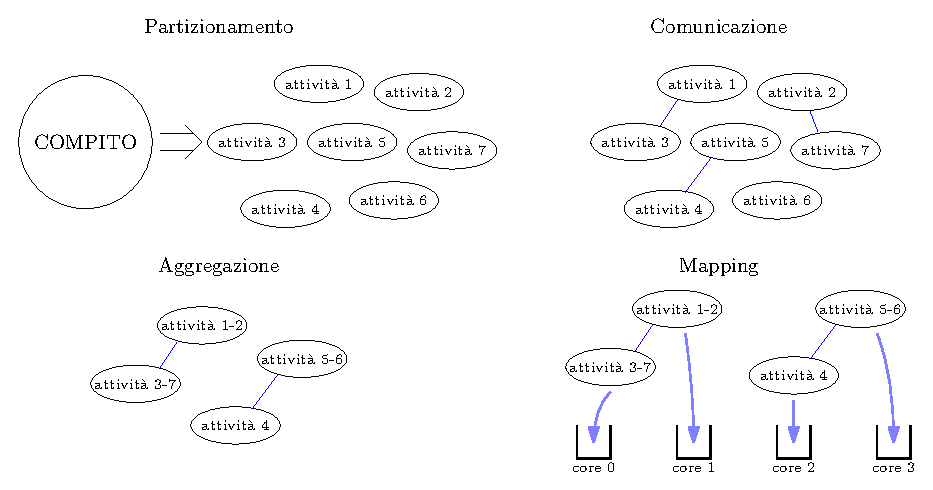
\includegraphics[width=0.9\textwidth]{images/foster.eps}
    \caption{Foster's methodology}
    \label{fig:foster}
\end{figure}
\begin{enumerate}
    \item \textit{Partizionamento} : si identificano delle attività di base indipendenti fra loro che possono essere
    eseguite in parallelo.
    \item \textit{Comunicazione} : determinare quali sono le attività stabilite nel punto precedente che per essere 
    eseguite necessitano di uno scambio di messaggi. 
    \item \textit{Aggregazione} : identificare le attività precedentemente stabilite che devono necessariamente essere 
    eseguite in sequenza, ed aggregarle in un unica attività.
    \item \textit{Mapping} : assegnare ai vari processi le attività definite in precedenza in modo che il carico di 
    lavoro sia uniformemente distribuito. Idealmente la comunicazione deve essere ridotta al minimo.
\end{enumerate}
\subsection{Pattern di Design Parallelo}
La struttura di un programma parallelo può essere definita secondo due pattern, si può dire che esistono due modi 
di \textit{parallelizzare} un programma \begin{itemize}
    \item \textbf{GPLS (Globally Parallel, Locally Sequential)} : L'applicazione vede diversi task sequenziali venire eseguiti in parallelo. 
    \item \textbf{GSLP (Globally Sequential, Locally Parallel)} : L'applicazione segue uno specifico "flusso" di esecuzione sequenziale, di cui 
    alcune parti vengono eseguite in parallelo.
\end{itemize}
\begin{figure}[h!]
    \centering
    \includegraphics[width=0.6\textwidth]{images/GPLSoGSLP.eps}
    \caption{GPLS e GSLP}
    \label{fig:GPLSoGSLP}
\end{figure}
\subsubsection{Esempi di GPLS}\begin{itemize}
    \item \textbf{Single Program Multiple Data} : La logica dell'applicazione viene mantenuta in un unico 
    eseguibile, tipicamente il programma segue la seguente struttura\begin{enumerate}
        \item Inizializzazione del programma 
        \item Ottenimento degli identificatori 
        \item Esecuzione del programma in diverse ramificazioni in base ai core coinvolti 
        \item Terminazione del programma
    \end{enumerate}
    \item \textbf{Multiple Program Multiple Data} : Quando la memoria da utilizzare è elevata è necessario suddividere 
    il carico su più programmi, che spesso vengono eseguiti su differenti piattaforme.
    \item \textbf{Master-Worker} : Ogni processo può essere \begin{itemize}
    \item Worker - Esegue la computazione
        \item Master - Gestisce il carico di lavoro e lo assegna ai processi worker, colleziona i risultati ottenuti 
        da questi ultimi e si occupa spesso delle operazioni di I/O o interazione con l'utente.
    \end{itemize}
    \item \textbf{Map-Reduce} : Una versione modificata del paradigma Master-Worker, in cui i nodi 
    worker eseguono due tipi di operazioni \begin{itemize}
        \item Map : Esegue la computazione su un insieme di dati che risulta in un insieme di risultati parziali (ad esempio, 
        esegue la somma su ogni elemento di un vettore) 
        \item Reduce : Colleziona i risultati parziali e ne deriva un risultato finale (ad esempio, somma tutti gli elementi di un 
        vettore ottenendo un unico scalare)
    \end{itemize}
\end{itemize}
\subsubsection{Esempi di GSLP}\begin{itemize}
    \item \textbf{Fork-Join} : C'è un unico "padre" in cui avviene l'esecuzione, quando necessario, 
    tale padre potrebbe eseguire una \code{fork} generando dei nodi figli, che eseguono la computazione 
    per poi terminare, facendo si che il padre continui.
    \item \textbf{Loop-Parallelism} : Risulta estremamente semplice da utilizzare e viene spesso applicata 
    quando un programma sequenziale deve essere adattato al multiprocesso. Consiste nel parallelizzare ogni 
    esecuzione di un ciclo \code{for}, è necessario che le iterazione però siano indipendenti fra loro.
\end{itemize}
\begin{lstlisting}[style=CStyle]
    //Esempio di Fork-Join
    mergesort(A,lo,hi){
        if lo < hi{
            mid = lo + (hi-lo) / 2 
            fork mergesort(A,lo,mid)
            mergesort(A,mid,hi)

            join 
            merge(A,lo,mid,hi)
        }
    }
\end{lstlisting}
\flowerLine 
\section{Comunicazione  non Bloccante e Comunicazione Collettiva}
Il contesto canonico di utilizzo di MPI è su un'insieme di server connessi fra loro (memoria privata), quando un 
processo esegue una \code{MPI\_Send}, il buffer in cui è contenuto il messaggio viene copiato e salvato dalla memoria 
principale alla memoria dell'interfaccia di rete (NIC Memory), per poi venire trasferito attraverso la rete verso la memoria 
NIC del destinatario, da li, verrà poi trasferita nella memoria principale di quest'ultimo. \acc 
L'utilizzo di una \code{MPI\_Send} è quindi dispendioso dal punto di vista computazionale, in quanto sono coinvolte 
molteplici operazioni di scrittura e chiamate di sistema, è quindi buona regola, eseguire il minor numero di 
\code{MPI\_Send} possibile\begin{quote}
    \color{gray}
    Ad esempio, è più conveniente eseguire una sola chiamata in cui si trasferiscono 200 byte piuttosto che due chiamate 
    in cui si trasferiscono 100 byte ciascuna.
    \color{black}
\end{quote}
Si è detto in precedenza che \code{MPI\_Send} è bloccante, in realtà, MPI utilizza, se non specificato diversamente, 
una metodologia di comunicazione standard, se il messaggio da trasferire è piccolo, è probabile che venga immediatamente 
trasferito venendo salvato su un buffer del destinatario. Diversamente, nel caso di un messaggio grande, la chiamata 
sarà bloccante in quanto MPI deve assicurarsi che il destinatario abbia allocato la memoria sufficente per riceverlo.\acc 
In entrambi i casi, MPI si assicura che il messaggio da inviare non vada perso, il programmma riottiene il controllo 
solo quando il buffer utilizzato per contenere il messaggio è di nuovo disponibile, si dice che la \code{MPI\_Send} 
è \textit{locally blocking}. Oltre la comunicazione standard, vi sono altri modi di inviare messaggi\begin{itemize}
    \item \textbf{Buffered} : Tramite la chiamata \code{MPI\_Bsend}, l'operazione è sempre locally blocking, ma l'utente deve fornire manualmente un 
    buffer in cui salvare il messaggio da inviare. 
    \item \textbf{Sincrona} : Tramite la chiamata \code{MPI\_Ssend}, l'operazione è globalmente bloccante, il controllo 
    viene restituito esclusivamente quando il destinatario ha ricevuto il messaggio chiamando \code{MPI\_Recv}. Risulta 
    utile per far si che un processo attenda che un altro arrivi ad un certo punto della computazione. 
    \item \textbf{Ready} : Tramite la chiamata \code{MPI\_Rsend}, se il destinatario non ha già effettuato una 
    \code{MPI\_Recv}, tale chiamata fallisce, è quindi necessario che esso sia già in attesa di ricevere.
\end{itemize}
\subsection{Send e Recv Immediate}
Le chiamate \code{MPI\_Recv} e \code{MPI\_Send} sono considerate poco performanti in quanto il processo chiamante 
potrebbe bloccare la sua esecuzione, in alcuni casi può essere utile una chiamata non bloccante per la trasmissione 
dei dati, soprattutto quando il mancato ricevimento di essi non causa errori nell'esecuzione del programma. Le funzioni non 
bloccanti messe a disposizione da MPI sono dette \textbf{funzioni immediate}, e permettono l'overlap fra 
computazione e comunicazione. Se al momento di una chiamata di ricevimento non ci sono dati da leggere, il programmatore 
dovrà gestire esplicitamente la situazione.\acc 
La chiamata \code{MPI\_Isend} ha gli stessi parametri della funzione non immediata, eccetto un parametro aggiuntivo, 
\code{MPI\_Request *req}, necessario per avere informazioni sullo status della chiamata.\acc 
La chiamata \code{MPI\_Irecv} ha gli stessi parametri della funzione non immediata, eccetto per l'assenza del 
parametro sullo status originario, e l'aggiunta del parametro 
\code{MPI\_Request *req}, necessario per avere informazioni sullo status della chiamata.\acc 
La funzione \code{int MPI\_Wait(MPI\_Request *request, MPI\_Status *status)} fa si che il processo si blocchi 
finché un invio o una ricezione non è andato a buon termine. È una chiamata bloccante.\acc 
La funzione \code{int MPI\_Test(MPI\_Request *request, int *flag, MPI\_Status *status)} controlla se una 
chiamata di invio o ricezione è andata o no a buon fine, salvando l'esito del risultato nel campo \code{flag}.\acc 
Esistono altre varianti di \code{Wait} e \code{Test} \begin{itemize}
    \item \code{Waitall} 
    \item \code{Waitany} 
    \item \code{Testany}
    \item etc...
\end{itemize}
\subsection{Esempi di Applicazione}
Il seguente esempio mostra un programma in cui $n$ processi (in questo caso 4) si scambiano informazioni 
in una configurazione "ad anello", in cui ognuno invia e riceve a/da i suoi vicini, l'utilizzo di chiamate non bloccanti 
è utile per evitare situazioni di deadlock.
\begin{lstlisting}[style=CStyle]
#include "mpi.h" 
#include <stdio.h> 
int main(void) { 
    int numtasks, rank, next, prev, buf[2]; 
    MPI_Request reqs[4]; // variabili necessarie per le chiamate Irecv e Isend
    MPI_Status stats[4]; // variabili necessarie per Waitall  
    MPI_Init(NULL, NULL); 
    MPI_Comm_size(MPI_COMM_WORLD, &numtasks); 
    MPI_Comm_rank(MPI_COMM_WORLD, &rank);
    // Determina vicino a sinistra e a destra
    prev = (rank-1) % numtasks; 
    next = (rank+1) % numtasks; 
    // Operazioni di comunicazione
    MPI_Irecv(&buf[0], 1, MPI_INT, prev, 0, MPI_COMM_WORLD, &reqs[0]); 
    MPI_Irecv(&buf[1], 1, MPI_INT, next, 0, MPI_COMM_WORLD, &reqs[1]); 
    MPI_Isend(&rank, 1, MPI_INT, prev, 0, MPI_COMM_WORLD, &reqs[2]); 
    MPI_Isend(&rank, 1, MPI_INT, next, 0, MPI_COMM_WORLD, &reqs[3]); 
    // Qui puo' essere eseguita computazione nel mentre che gli altri processi comunicano
    // Attende la fine delle operazioni non bloccanti
    MPI_Waitall(4, reqs, stats); 
    MPI_Finalize(); 
}
\end{lstlisting}
\begin{center}
    \begin{figure}[h!]
        \center
        \includegraphics[width=0.5\textwidth]{images/ring.eps}
        \caption{configurazione ad anello}
        \label{fig:ring}
    \end{figure}
\end{center}
\subsubsection{Integrazione numerica}\label{integrale}
Si consideri adesso il seguente esempio, si vuole scrivere un programma che esegua l'integrazione numerica 
di una generica funzione $f(x)$ tramite la regola del trapezoide. Tale metodo consiste nel dividere l'intervallo 
di integrazione in $n$ intervalli $$\{(x_0,x_1),(x_1,x_2),(x_2,x_3)\dots (x_{n-1},x_n)\}$$ lunghi $h$,
 di cui verrà calcolata l'area approssimandola ad un trapezio.
 \begin{center}
    \includegraphics[width=0.8\textwidth]{images/trapezio.eps}
 \end{center}
L'integrale approssimato sarà la somma totale di tutti i trapezoidi 
$$ \frac{h}{2}\Big[[f(x_1)+f(x_{2})]+[f(x_2)+f(x_{3})]+\dots +[f(x_{n-1})+f(x_{n})]\Big]$$
\begin{lstlisting}[style=CStyle]
/* Input : a, b, n */
h = (b-a)/n;
approx = (f(a)+f(b))/2;
for(i=1;i<=n-1;i++){
    x_i = a+i*h; 
    approx += f(x_i);
}
approx=h*approx;
\end{lstlisting}
Se ne vuole dare un'implementazione parallela in cui i vari processi eseguiranno il calcolo di un 
trapezio, le somme parziali verranno inviate al processo di rank 0 che si occuperà di calcolare 
la somma totale (paradigma MAP REDUCE).
\begin{lstlisting}[style=CStyle]
double Trap(double left, double right, int count, double base_len){

    double esitmate, x;
    // f e' la funzione integranda
    esitmate = (f(left)+f(right))/2.0;
    for(int i = 1; i<=count-1; i++){
        x=left+i*base_len;
        estimate+=f(x);
    }
    return estimate*base_len;
}
\end{lstlisting}
\begin{lstlisting}[style=CStyle]
int main(void){

    int my_rank; 
    int comm_size;
    int n = 1024; //numero di intervalli, piu' e' grande, piu' la stima sara' precisa 
    double a = 0.0; //estremo sinistro di integrazione
    double b = 3.0; //estremo destro di integrazione
    double h; //lunghezza intervalli; 
    double local_a, local b;
    double local_sum;
    double total_sum;
    int source;

    MPI_Init(NULL,NULL);
    MPI_Comm_rank(MPI_COMM_WORLD,&my_rank);
    MPI_Comm_size(MPI_COMM_WORLD,&comm_size);

    h=(b-a)/n; 
    local_n = n/comm_size; //numero di trapezoidi per ogni processo 

    local_a = a+my_rank*local_n*h;
    local_b=local_a+local_n*h;
    local_sum = Trap(local_a, local_b, local_n, h); //calcolo somma parziale

    if(my_rank!=0){
        //Invio la somma parziale al processo con rank 0
        MPI_Send(&local_sum, 1, MPI_DOUBLE, 0, 0, MPI_COMM_WORLD);
    }
    else{
        total_sum = local_sum;
        for(source = 1;source<comm_sz; source++){
            MPI_Recv(&local_sum, 1, MPI_DOUBLE, source, 0,
                         MPI_COMM_WORLD, MPI_STATUS_IGNORE);
            total_sum+=local_sum
        }

        printf("con n = %d trapezoidi, la somma approssimata della funzione\n  
               da %f a %f e' %.15e .\n", n, a, b, total_sum);
    }

    MPI_Finalize();
    return 0;
}
\end{lstlisting}
\subsection{Operazioni Collettive}
Qual'è il problema con l'implementazione del trapezoide appena mostrata? Il processo di rank zero ha un carico di lavoro superiore 
rispetto ogni altro processo, infatti, quest'ultimo oltre la somma dei suoi trapezi locali, deve calcolare 
la somma totale, inoltre deve occuparsi di ricevere i dati da tutti gli altri processi. 
\begin{figure}[h!]
    \centering
    \includegraphics[width=450pt]{images/tree2.eps}
    \caption{alberi differenti (entrambi validi)}
    \label{fig:tree_cores2}
\end{figure}\acc
Si può pensare di 
suddividere il carico di lavoro ad albero, come già visto in figura 
\ref{fig:tree_cores}, facendo si che il suo carico di lavoro sia logaritmico in funzione del numero dei rank. 
Nell'esempio visto, ogni processo condivide i suoi dati parziali con quello adiacente (da un punto di vista 
di numero di identificazione), ma nulla vieta agli ultimi processi di condividere i dati con i primi, come in figura 
\ref{fig:tree_cores2}.
L'ottimalità di una soluzione piuttosto che di un altra può dipendere da diversi fattori non sempre analizzabili, come 
la topologia fisica della reta attraverso cui sono collegate le macchine che eseguono i processi.\acc 
A tal proposito, MPI fornisce una funzionalità che permette di eseguire operazioni di aggregazione di risultati 
senza preoccuparci della logica di comunicazione per il trasferimento dei dati parziali. La funzione in questione è 
\code{int MPI\_Reduce}, con i seguenti parametri
\begin{itemize}
    \item \code{void* input\_data\_o} è il puntatore alla variabile in ingresso (somma parziale)
    \item \code{void* output\_data\_o} è il puntatore al valore che sarà riempito con il valore totale aggregato
    \item \code{int count} è il numero di elementi da aggregare
    \item \code{MPI\_Datatype datatype} è il tipo dei valori in questione
    \item \code{MPI\_Op operator} è l'operazione di aggregazione (somma, moltiplicazione, XOR, etc...) 
    \item \code{int dest\_process} è il rank del processo che riceverà il risultato
    \item \code{MPI\_Comm comm} il comunicatore in questione
\end{itemize}
Le operazioni di aggregazione supportate da MPI sono le seguenti \begin{center}
    \begin{tabular}{|l|l|}
        \hline
        \rowcolor[HTML]{6434FC} 
        {\color[HTML]{FFFFFF} Operazione}     & {\color[HTML]{FFFFFF} Significato} \\ \hline
        \texttt{MPI\_MAX}    & Massimo                            \\ \hline
        \texttt{MPI\_MIN}    & Minimo                             \\ \hline
        \texttt{MPI\_SUM}    & Somma                              \\ \hline
        \texttt{MPI\_PROD}   & Prodotto                           \\ \hline
        \texttt{MPI\_LAND}   & AND logico                         \\ \hline
        \texttt{MPI\_BAND}   & AND bit a bit                      \\ \hline
        \texttt{MPI\_LOR}    & OR logico                          \\ \hline
        \texttt{MPI\_BOR}    & OR bit a bit                       \\ \hline
        \texttt{MPI\_LXOR}   & XOR logico                         \\ \hline
        \texttt{MPI\_BXOR}   & XOR bit a bit                      \\ \hline
        \texttt{MPI\_MAXLOC} & Massimo insieme al suo indice      \\ \hline
        \texttt{MPI\_MINLOC} & Minimo insieme al suo indice       \\ \hline
        \end{tabular}
\end{center}
È possibile anche definire delle operazioni personalizzate tramite la chiamata \code{MPI\_Op\_create}.\acc 
Quando viene chiamata una funzione collettiva, è importante che ogni processo del comunicatore la chiami, altrimenti 
l'esecuzione rimane bloccata in uno stato di attesa, dato che ogni processo attende che tutti gli altri siano arrivati 
a tale operazione. Ovviamente, tutti i processi che eseguono un'operazione di questo tipo devono definire lo 
stesso processo che riceverà l'output. Tutti i processi escluso quello di destinazione, nel campo 
\code{void* output\_data\_o} possono specificare qualsiasi valore.\acc 
Non essendo presente alcun tag, nella comunicazione collettiva, le operazioni verranno matchate in base all'ordine 
di esecuzione. Nell'esempio del trapezoide \ref{integrale} vi è un problema, nel caso si volesse decidere arbitrariamente 
l'intervallo di integrazione, o il numero di trapezi, il processo di rank 0 dovrà occuparsi di leggere i dati da stdin, per poi 
condividerli ad ogni altro processo.\begin{quote}
    \color{gray}Si ricordi che in MPI, esclusivamente il processo di rank 0 può interagire con lo stdin.\color{black}
\end{quote}
È chiaro che su di esso sia riportato un carico di lavoro maggiore, è quindi possibile suddividere il carico facendo si 
che il processo 0 condivida i dati con due altri processi, e questi due li condividano a loro volta con altri due processi ciascuno, 
creando un albero di condivisione.\begin{center}
    \includegraphics[width=0.5\textwidth]{images/tree3.eps}
\end{center}
Anche in questo caso, la logica con la quale scambiarsi le informazioni può variare, e quella ottimale può dipendere 
dalle condizioni della rete ed altri fattori difficilmente analizzabili, per questo MPI fornisce una funzione, 
\code{MPI\_Bcast} che si occupa di eseguire il broadcast da un processo verso tutti gli altri. I parametri sono 
i seguenti : \begin{itemize}
    \item \code{void* data\_p} è il puntatore alla variabile da condividere
    \item \code{int count} è il numero di elementi da condividere
    \item \code{MPI\_Datatype datatype} è il tipo dei valori in questione
    \item \code{int source\_process} è il rank del processo che condivide il valore
    \item \code{MPI\_Comm comm} il comunicatore in questione
\end{itemize}
Il parametro \code{void* data\_p} fungerà sia da input, che da output, nel caso il processo chiamante sia 
colui che condivide il valore, in \code{data\_p} sarà presente il valore condiviso, altrimenti, in \code{data\_p}  
sarà presente il valore ricevuto.\acc 
Esempio di funzione per leggere input da tastiera 
\begin{lstlisting}[style=CStyle]
    void Get_input(int my_rank, a, int b, int n){
        if(my_rank==0){
            printf("enter input:\n");
            scanf("%d %d %d",a , b, n);
        }
        MPI_Bcast(a, 1, MPI_INT, 0, MPI_COMM_WORLD);
        MPI_Bcast(b, 1, MPI_INT, 0, MPI_COMM_WORLD);
        MPI_Bcast(n, 1, MPI_INT, 0, MPI_COMM_WORLD);
    }
\end{lstlisting}
A questo punto, si supponga di voler fare un operazione di aggregato, per poi avere il risultato condiviso fra tutti 
i processi, concettualmente, ciò equivale ad eseguire una \code{MPI\_Reduce} seguita da una \code{MPI\_Bcast}. MPI 
fornisce una funzione a tal proposito, ottimizzata a dovere, ossia \code{MPI\_Allreduce}, con i seguenti parametri\begin{itemize}
    \item \code{void* input\_data\_o} è il puntatore alla variabile in ingresso (somma parziale)
    \item \code{void* output\_data\_o} è il puntatore al valore che sarà riempito con il valore totale aggregato
    \item \code{int count} è il numero di elementi da aggregare
    \item \code{MPI\_Datatype datatype} è il tipo dei valori in questione
    \item \code{MPI\_Op operator} è l'operazione di aggregazione (somma, moltiplicazione, XOR, etc...) 
    \item \code{MPI\_Comm comm} il comunicatore in questione
\end{itemize}
I parametri sono identici alla \code{MPI\_Reduce},  eccetto per l'assenza del processo di destinazione, dato che 
in questo caso, ogni processo avrà il risultato.\acc 
Le operazioni collettive sono diventate particolarmente importanti nell'ultimo periodo in quanto sono 
utilizzate nella stragrande maggioranza dei programmi paralleli che vengono eseguiti per il training delle 
reti neurali odierne. Le grosse aziende di informatica, hanno iniziato a produrre delle proprie librerie 
proprietarie\begin{itemize}
    \item NCCL (\textit{Nvidia})
    \item RCCL (\textit{AMD})
    \item OneCCL (\textit{Intel})
    \item MSCCL (\textit{Microsoft})
\end{itemize}
MPI durante le operazioni aggregate utilizza delle euristiche per stimare quale sia il miglior modo di condividere 
i dati fra i nodi, è possibile forzare tale decisione attraverso delle opportune variabili d'ambiente. Il punto è che MPI
non è consapevole dell'hardware sul quale i processi sono eseguiti, per questo le aziende hanno iniziato a 
produrre librerie proprietarie, appositamente ottimizzate per girare sulle piattaforme dedicate.
\subsubsection{Stima del $\pi$}
Si vuole scrivere un programma che tramite il metodo di Montecarlo calcoli il valore stimato di $\pi$ distribuendo il 
lavoro su più processi tramite MPI. L'algoritmo utilizzato per il calcolo è semplice, si consideri un cerchio di 
raggio unitario, inscritto in un quadrato $2\times 2$.\begin{center}
    
\includegraphics[width=0.5\textwidth]{images/cerchio.eps}
\end{center}
L'area del cerchio, è uguale a $\pi r^2\implies \pi$, l'area del quadrato è $4$. Sia $A_c$ l'insieme di tutti i 
punti compresi nel cerchio, e sia $A_q$ l'insieme di tutti i punti compresi nel quadrato. Risulta che il numero di punti 
nell'area del cerchio stanno all'area $\pi$, come il numero di punti che stanno nell'area del quadrato stanno a $4$.
$$ \dfrac{|A_c|}{\pi}=\dfrac{|A_q|}{4}$$
In realtà, non ha senso considerare la cardinalità di $|A_c|$ o di $|A_q|$, in quanto sono insiemi infiniti, supponiamo allora 
che tali insiemi siano finiti e di cardinalità $n$, si denotano $A_c^n$ e $A_q^n$, chiaramente $A_c^n\subseteq A_q^n$. 
Si ha che 
$$ \lim_{n\rightarrow \infty} 4\cdot \dfrac{|A_c^n|}{|A_q^n|} = \pi$$
L'algoritmo consiste nel calcolare un numero $n$ di punti casuali, sia $c$ il numero di punti interni al cerchio, ossia 
i punti $(x,y)$ tali da rispettare $x^2+y^2\le 1$. Numericamente, $4\dfrac{n}{c}$ approssimerà $\pi$, con una precisione 
sempre maggiore all'aumentare di $n$.\acc 
L'algoritmo si renderà parallelo, distribuendo equamente il numero di punti da calcolare a tutti i processi presenti.
\begin{lstlisting}[style=CStyle]
    #include <stdio.h>
    #include <stdlib.h>
    #include <mpi.h>
    #include <time.h>
    
    int main(int argc, char **argv)
    {
    
        int precision = 1000; // Numero di punti generati casualmente
    
        if (argc > 1)
        {
            precision = atoi(argv[1]);
        }
    
        MPI_Init(NULL, NULL);
        srand(time(NULL));
    
        int my_rank;
        int my_size;
        MPI_Comm_rank(MPI_COMM_WORLD, &my_rank);
        MPI_Comm_size(MPI_COMM_WORLD, &my_size);
    
        int local_precision = precision / my_size; /* Numero di punto da generare per
                                                      ogni processo */
        int local_circle_point = 0;
    
        for (int i = 0; i <= local_precision; i++)
        {
            double x = (double)rand() / RAND_MAX * 2.0 - 1.0; // Generazione punto
            double y = (double)rand() / RAND_MAX * 2.0 - 1.0;
            if (x * x + y * y < 1) // Controllo se il punto e' nel cerchio
                local_circle_point++;
        }
    
        int total_circle_point = 0;
        MPI_Reduce(&local_circle_point, &total_circle_point, 1, MPI_INT, MPI_SUM,
                                                               0, MPI_COMM_WORLD);
    
        if (my_rank == 0)
        {
            double esteem = ((double)total_circle_point / precision * 4);
            printf("Su %d precision, la stima del pi greco e' : %lf\n",
                                                    precision, esteem);
        }
    
        MPI_Finalize();
        return 0;
    }
\end{lstlisting}\large\begin{center}
    \begin{tabular}{ll}
        \rowcolor[HTML]{FFFFFF} 
        \multicolumn{2}{c}{\cellcolor[HTML]{FFFFFF}Risultati della Computazione}                                                              \\
        \rowcolor[HTML]{CBCEFB} 
        \multicolumn{1}{c|}{\cellcolor[HTML]{CBCEFB}Numero punti generati} & \multicolumn{1}{c}{\cellcolor[HTML]{CBCEFB}Valore $\pi$ stimato} \\
        \rowcolor[HTML]{ECF4FF} 
        \multicolumn{1}{l|}{\cellcolor[HTML]{ECF4FF}100}                   & 4.08                                                             \\
        \rowcolor[HTML]{DAE8FC} 
        \multicolumn{1}{l|}{\cellcolor[HTML]{DAE8FC}1000}                  & 3.408                                                            \\
        \rowcolor[HTML]{ECF4FF} 
        \multicolumn{1}{l|}{\cellcolor[HTML]{ECF4FF}10000}                 & 3.1031                                                           \\
        \rowcolor[HTML]{DAE8FC} 
        \multicolumn{1}{l|}{\cellcolor[HTML]{DAE8FC}100000}                & 3.13416                                                          \\
        \rowcolor[HTML]{ECF4FF} 
        \multicolumn{1}{l|}{\cellcolor[HTML]{ECF4FF}1000000}               & 3.143736                                                         \\
        \rowcolor[HTML]{DAE8FC} 
        \multicolumn{1}{l|}{\cellcolor[HTML]{DAE8FC}100000000}             & 3.141725                                                        
        \end{tabular}
\end{center}\normalsize 
\flowerLine 
\section{Valutazione del Tempo}
Valutare il tempo di esecuzione di un programma multicore 
non è banale. MPI fornisce una funzione \code{double MPI\_Wtime}, 
ritorna un valore che rappresenta il tempo passato da un certo 
riferimento fisso. Basta valutare questo tempo in due punti diversi 
del codice e farne la differenza.
\begin{lstlisting}[style=CStyle]
    double start,finish;
    start=MPI_Wtime();
    /*codice*/
    finish=MPI_Wtime();
    printf("%d",finish-start);
\end{lstlisting}
Ogni processo, seguirà un evoluzione dello stesso codice differente, e 
non contemporanea fra gli altri. Se verrà calcolato il tempo 
trascorso per l'esecuzione di una sezione di codice, ogni processo 
resituirà un tempo diverso. Il tempo totale del programma, sarà 
dato dal massimo dei tempi forniti da ogni processo. Si può usare 
l'operazione collettiva 
\begin{lstlisting}[style=CStyle]
    double local_start,local_finish,local_elapsed,elapsed;
    local_start=MPI_Wtime();
    /*codice*/
    local_finish=MPI_Wtime();
    local_elapsed=local_finish-local_start;
    MPI_Reduce(&local_elapsed,&elapsed,1,MPI_DOUBLE,MPI_MAX,0,comm);
    printf("%d",elapsed);
\end{lstlisting}
Ovviamente, tale metodo è valido con l'assunzione che tutti i processi 
inizino nello stesso momento (in particolare, la valutazione del 
tempo di inizio), un'esecuzione reale però è sfasata, e 
ciò porterebbe ad un tempo di esecuzione che non corrisponde a quello 
effettivo.\acc 
Quando si esegue un'operazione di reduce, tutti i processi 
devono arrivare ad uno punto comune nel codice, "sincronizzandosi", 
esiste un'operazione, \code{MPI\_Barrier}, il cui unico scopo è attendere che tutti i processi 
la eseguano prima di continuare nell'esecuzione. Tale operazione comunque, 
non garantisce che i processi si sincronizzino una volta eseguita, quindi 
approssima il comportamento sincronizzato. Nella pratica, è molto 
complesso garantire tale proprietà.\acc 
La misurazione del tempo impiegato da un processo è 
non deterministica, in quanto quest'ultimo è 
soggetto alle interruzioni del sistema operativo ed ai cambi di 
contesto, che possono variare in maniera apparentemente aleatoria. Nel 
caso in cui il programma venga eseguito in rete, tale \textit{rumore} 
(il tempo casuale aggiunto all'esecuzione normale di un processo) è ancora maggiore.
\acc Generalmente, è corretto eseguire più volte un processo misurando 
i tempi ad ogni esecuzione, per avere una misura statistica. Il minimo 
corrisponderà al caso ideale, il massimo al caso peggiore, la mediana al caso più 
frequente, è corretto fornire i dati di ogni esecuzione per avere 
un quadro chiaro dei tempi effettivi. In breve per valutare il tempo \begin{enumerate}
    \item Si mette una funzione barriera all'inizio dell'esecuzione 
    \item Si trova il massimo dei tempi di ogni processo 
    \item Si provano diverse esecuzioni ottenendo una distribuzione
\end{enumerate}
\begin{center}
    \includegraphics[width=0.5\textwidth]{images/distribuzioni.eps}
\end{center}
Le interferenze ed i rumori sono stati grande oggetto di studio 
nella valutazione dei tempi, in particolare, si è osservato un rapporto 
di proporzionalità diretta fra il rumore ed il numero di processi 
impiegati in un calcolo, esiste quindi un limite, in cui 
l'aumento dei nodi volti ad un calcolo non garantisce un 
miglioramento dei tempi di esecuzione, bensì il contrario.
\acc 
La seguente tabella, raccoglie i tempi di esecuzione in secondi di un algoritmo 
che esegue il prodotto fra matrici quadrate.\begin{center}
    \begin{tabular}{c|ccccc|}
        \cline{2-6}
        tempo (sec)                                                              & \multicolumn{5}{c|}{\cellcolor[HTML]{ECF4FF}ordine della matrice}                                                                                                                                                     \\ \hline
        \rowcolor[HTML]{ECF4FF} 
        \multicolumn{1}{|c|}{\cellcolor[HTML]{FFFFC7}numero processi} & \multicolumn{1}{c|}{\cellcolor[HTML]{ECF4FF}1024} & \multicolumn{1}{c|}{\cellcolor[HTML]{ECF4FF}2048} & \multicolumn{1}{c|}{\cellcolor[HTML]{ECF4FF}4096} & \multicolumn{1}{c|}{\cellcolor[HTML]{ECF4FF}8192} & 16384 \\ \hline
        \multicolumn{1}{|c|}{\cellcolor[HTML]{FFFFC7}1}               & \multicolumn{1}{c|}{4.1}                          & \multicolumn{1}{c|}{16}                           & \multicolumn{1}{c|}{64}                           & \multicolumn{1}{c|}{270}                          & 1100  \\ \hline
        \multicolumn{1}{|c|}{\cellcolor[HTML]{FFFFC7}2}               & \multicolumn{1}{c|}{2.3}                          & \multicolumn{1}{c|}{8.5}                          & \multicolumn{1}{c|}{33}                           & \multicolumn{1}{c|}{140}                          & 560   \\ \hline
        \multicolumn{1}{|c|}{\cellcolor[HTML]{FFFFC7}4}               & \multicolumn{1}{c|}{2}                            & \multicolumn{1}{c|}{5.1}                          & \multicolumn{1}{c|}{18}                           & \multicolumn{1}{c|}{70}                           & 280   \\ \hline
        \multicolumn{1}{|c|}{\cellcolor[HTML]{FFFFC7}8}               & \multicolumn{1}{c|}{1.7}                          & \multicolumn{1}{c|}{3.3}                          & \multicolumn{1}{c|}{9.8}                          & \multicolumn{1}{c|}{36}                           & 140   \\ \hline
        \multicolumn{1}{|c|}{\cellcolor[HTML]{FFFFC7}16}              & \multicolumn{1}{c|}{1.7}                          & \multicolumn{1}{c|}{2.6}                          & \multicolumn{1}{c|}{5.9}                          & \multicolumn{1}{c|}{19}                           & 71    \\ \hline
        \end{tabular}
\end{center}
Ovviamente, con l'aumento delle dimensioni dell'input, aumenta anche il tempo di esecuzione, e quest'ultimo 
decresce con l'aumentare del numero di processi. Questo fattore di proporzionalità inversa non è però 
valido per un arbitrario numero di processo, de facto, ci sarà un limite per cui vale, ad un certo punto, 
l'aumentare dei processi non migliorerà il tempo di esecuzione. Per la stima dei tempi si definiscono le 
seguenti variabili \begin{itemize}
    \item $T_s(n)$ è il tempo di esecuzione di un programma se eseguito in maniera sequenziale, con un 
    input di dimensione $n$. 
    \item $T_p(n,p)$ è il tempo di esecuzione di un programma se eseguito in maniera parallela con $p$ processi,
    e con un 
    input di dimensione $n$. 
    \item $S(n,p)=\dfrac{T_s(n)}{T_p(n,p)}$ è detto \textbf{speed up} dell'applicazione e misura il margine di 
    miglioramento di un programma quando si esegue in parallelo piuttosto che in sequenziale.
\end{itemize}
Ovviamente nel rapporto dello speed up i tempi sequenziali e paralleli vanno misurati sullo stesso 
hardware. L'ideale sarebbe uno speed up lineare, nell'effettivo, l'aumentare dei processi 
fa diminuire lo speed up, invece l'aumentare dell'input lo fa aumentare. La seguente tabella riporta i valori 
dello speed up del programma che esegue il prodotto fra matrici.\begin{center}
    \begin{tabular}{c|ccccc|}
        \cline{2-6}
        speed up                                                      & \multicolumn{5}{c|}{\cellcolor[HTML]{ECF4FF}ordine della matrice}                                                                                                                                                     \\ \hline
        \rowcolor[HTML]{ECF4FF} 
        \multicolumn{1}{|c|}{\cellcolor[HTML]{FFFFC7}numero processi} & \multicolumn{1}{c|}{\cellcolor[HTML]{ECF4FF}1024} & \multicolumn{1}{c|}{\cellcolor[HTML]{ECF4FF}2048} & \multicolumn{1}{c|}{\cellcolor[HTML]{ECF4FF}4096} & \multicolumn{1}{c|}{\cellcolor[HTML]{ECF4FF}8192} & 16384 \\ \hline
        \multicolumn{1}{|c|}{\cellcolor[HTML]{FFFFC7}1}               & \multicolumn{1}{c|}{1}                            & \multicolumn{1}{c|}{1}                            & \multicolumn{1}{c|}{1}                            & \multicolumn{1}{c|}{1}                            & 1     \\ \hline
        \multicolumn{1}{|c|}{\cellcolor[HTML]{FFFFC7}2}               & \multicolumn{1}{c|}{1.8}                          & \multicolumn{1}{c|}{1.9}                          & \multicolumn{1}{c|}{1.9}                          & \multicolumn{1}{c|}{1.9}                          & 2     \\ \hline
        \multicolumn{1}{|c|}{\cellcolor[HTML]{FFFFC7}4}               & \multicolumn{1}{c|}{2.1}                          & \multicolumn{1}{c|}{3.1}                          & \multicolumn{1}{c|}{3.6}                          & \multicolumn{1}{c|}{3.9}                          & 3.9   \\ \hline
        \multicolumn{1}{|c|}{\cellcolor[HTML]{FFFFC7}8}               & \multicolumn{1}{c|}{2.4}                          & \multicolumn{1}{c|}{4.8}                          & \multicolumn{1}{c|}{6.5}                          & \multicolumn{1}{c|}{7.5}                          & 7.9   \\ \hline
        \multicolumn{1}{|c|}{\cellcolor[HTML]{FFFFC7}16}              & \multicolumn{1}{c|}{2.4}                          & \multicolumn{1}{c|}{6.2}                          & \multicolumn{1}{c|}{10.8}                         & \multicolumn{1}{c|}{14.2}                         & 15.5  \\ \hline
        \end{tabular}
\end{center}
Nota bene : $T_p(n,1)\ne T_s(n)$, generalmente il tempo di esecuzione parallela con 1 processo è maggiore del tempo 
di esecuzione sequenziale (dato che il setup dell'ambiente per il calcolo parallelo ha un costo).\acc 
La \textbf{scalabilità} di un processo è definita come segue 
$$ Sc(n,p)=\frac{T_p(n,1)}{T_p(n,p)}$$
L'\textbf{efficienza} invece è un valore compreso fra zero ed 1 definito come segue 
$$ E(n,p)=\frac{S(n,p)}{p}\in(0,1]$$\begin{center}
    \begin{tabular}{c|ccccc|}
        \cline{2-6}
        efficienza                                                    & \multicolumn{5}{c|}{\cellcolor[HTML]{ECF4FF}ordine della matrice}                                                                                                                                                     \\ \hline
        \rowcolor[HTML]{ECF4FF} 
        \multicolumn{1}{|c|}{\cellcolor[HTML]{FFFFC7}numero processi} & \multicolumn{1}{c|}{\cellcolor[HTML]{ECF4FF}1024} & \multicolumn{1}{c|}{\cellcolor[HTML]{ECF4FF}2048} & \multicolumn{1}{c|}{\cellcolor[HTML]{ECF4FF}4096} & \multicolumn{1}{c|}{\cellcolor[HTML]{ECF4FF}8192} & 16384 \\ \hline
        \multicolumn{1}{|c|}{\cellcolor[HTML]{FFFFC7}1}               & \multicolumn{1}{c|}{1}                            & \multicolumn{1}{c|}{1}                            & \multicolumn{1}{c|}{1}                            & \multicolumn{1}{c|}{1}                            & 1     \\ \hline
        \multicolumn{1}{|c|}{\cellcolor[HTML]{FFFFC7}2}               & \multicolumn{1}{c|}{0.89}                         & \multicolumn{1}{c|}{0.94}                         & \multicolumn{1}{c|}{0.97}                         & \multicolumn{1}{c|}{0.96}                         & 0.98  \\ \hline
        \multicolumn{1}{|c|}{\cellcolor[HTML]{FFFFC7}4}               & \multicolumn{1}{c|}{0.51}                         & \multicolumn{1}{c|}{0.78}                         & \multicolumn{1}{c|}{0.89}                         & \multicolumn{1}{c|}{0.96}                         & 0.98  \\ \hline
        \multicolumn{1}{|c|}{\cellcolor[HTML]{FFFFC7}8}               & \multicolumn{1}{c|}{0.3}                          & \multicolumn{1}{c|}{0.61}                         & \multicolumn{1}{c|}{0.82}                         & \multicolumn{1}{c|}{0.94}                         & 0.98  \\ \hline
        \multicolumn{1}{|c|}{\cellcolor[HTML]{FFFFC7}16}              & \multicolumn{1}{c|}{0.15}                         & \multicolumn{1}{c|}{0.39}                         & \multicolumn{1}{c|}{0.68}                         & \multicolumn{1}{c|}{0.89}                         & 0.97  \\ \hline
        \end{tabular}
\end{center}
Chiaramente, se le dimensioni dell'input sono modeste, l'utilizzo di tanti processi risulta inutile, 
l'efficienza è quindi bassa. L'utilizzo del multi processo ha senso quando l'input è di grande dimensione, 
e si presta ad essere diviso e computato da nodi paralleli.
\subsection{Scalabilità Forte e Scalabilità Debole}
Un programma si dice \textbf{strongly scalable} (fortemente scalabile) se, data una dimensione 
fissa dell'input $n$,  lo speed up ha una buona crescita all'aumentare dei processi. È invece 
\textbf{weakly scalable} (debolmente scalabile) se, l'aumentare dell'input, e l'aumentare del numero dei processi, 
il tempo di esecuzione varia di poco.\acc 
Rendere un applicazione strongly scalable è estremamente difficile, per questo nell'effettivo viene considerato 
sempre il weak scaling quando si vuole parallelizzare un compito. È possibile avere una stima approssimativa
 di quanto un'applicazione possa scalare? Dato un programma, si definisce \textbf{frazione seriale} 
 la porzione di esso che è impossibile da parallelizzare, e viene espressa come un valore fra 0 ed 1. 
 Tale parte non potrà essere influenzata dalla parallelizzazione, la \textbf{legge di Amdahl} stabilisce che lo 
 scaling di un'applicazione è limitato dalla frazione seriale. Per un $n$ dimensione in input fissata, si ha
 $$ T_p(p)=(1-\alpha)T_s+\alpha\frac{T_s}{p}$$
 Dove $\alpha\in[0,1]$ rappresenta la frazione parallelizzabile, e $1-\alpha$ la frazione seriale. Lo speed up 
 sarà quindi 
 $$ S(p)=T_s\frac{1}{(1-\alpha)T_s+\alpha\frac{T_s}{p}}$$
 Il valore dello speed up è limitato superiormente, infatti all'aumentare dei processi :
\begin{eqnarray}
    \lim_{p\rightarrow\infty}S(p) = \\ 
    \lim_{p\rightarrow\infty}T_s\frac{1}{(1-\alpha)T_s+\alpha\frac{T_s}{p}} = \\ 
    \frac{T_s}{(1-\alpha)T_s}=\frac{1}{1-\alpha}
\end{eqnarray}\begin{center}
    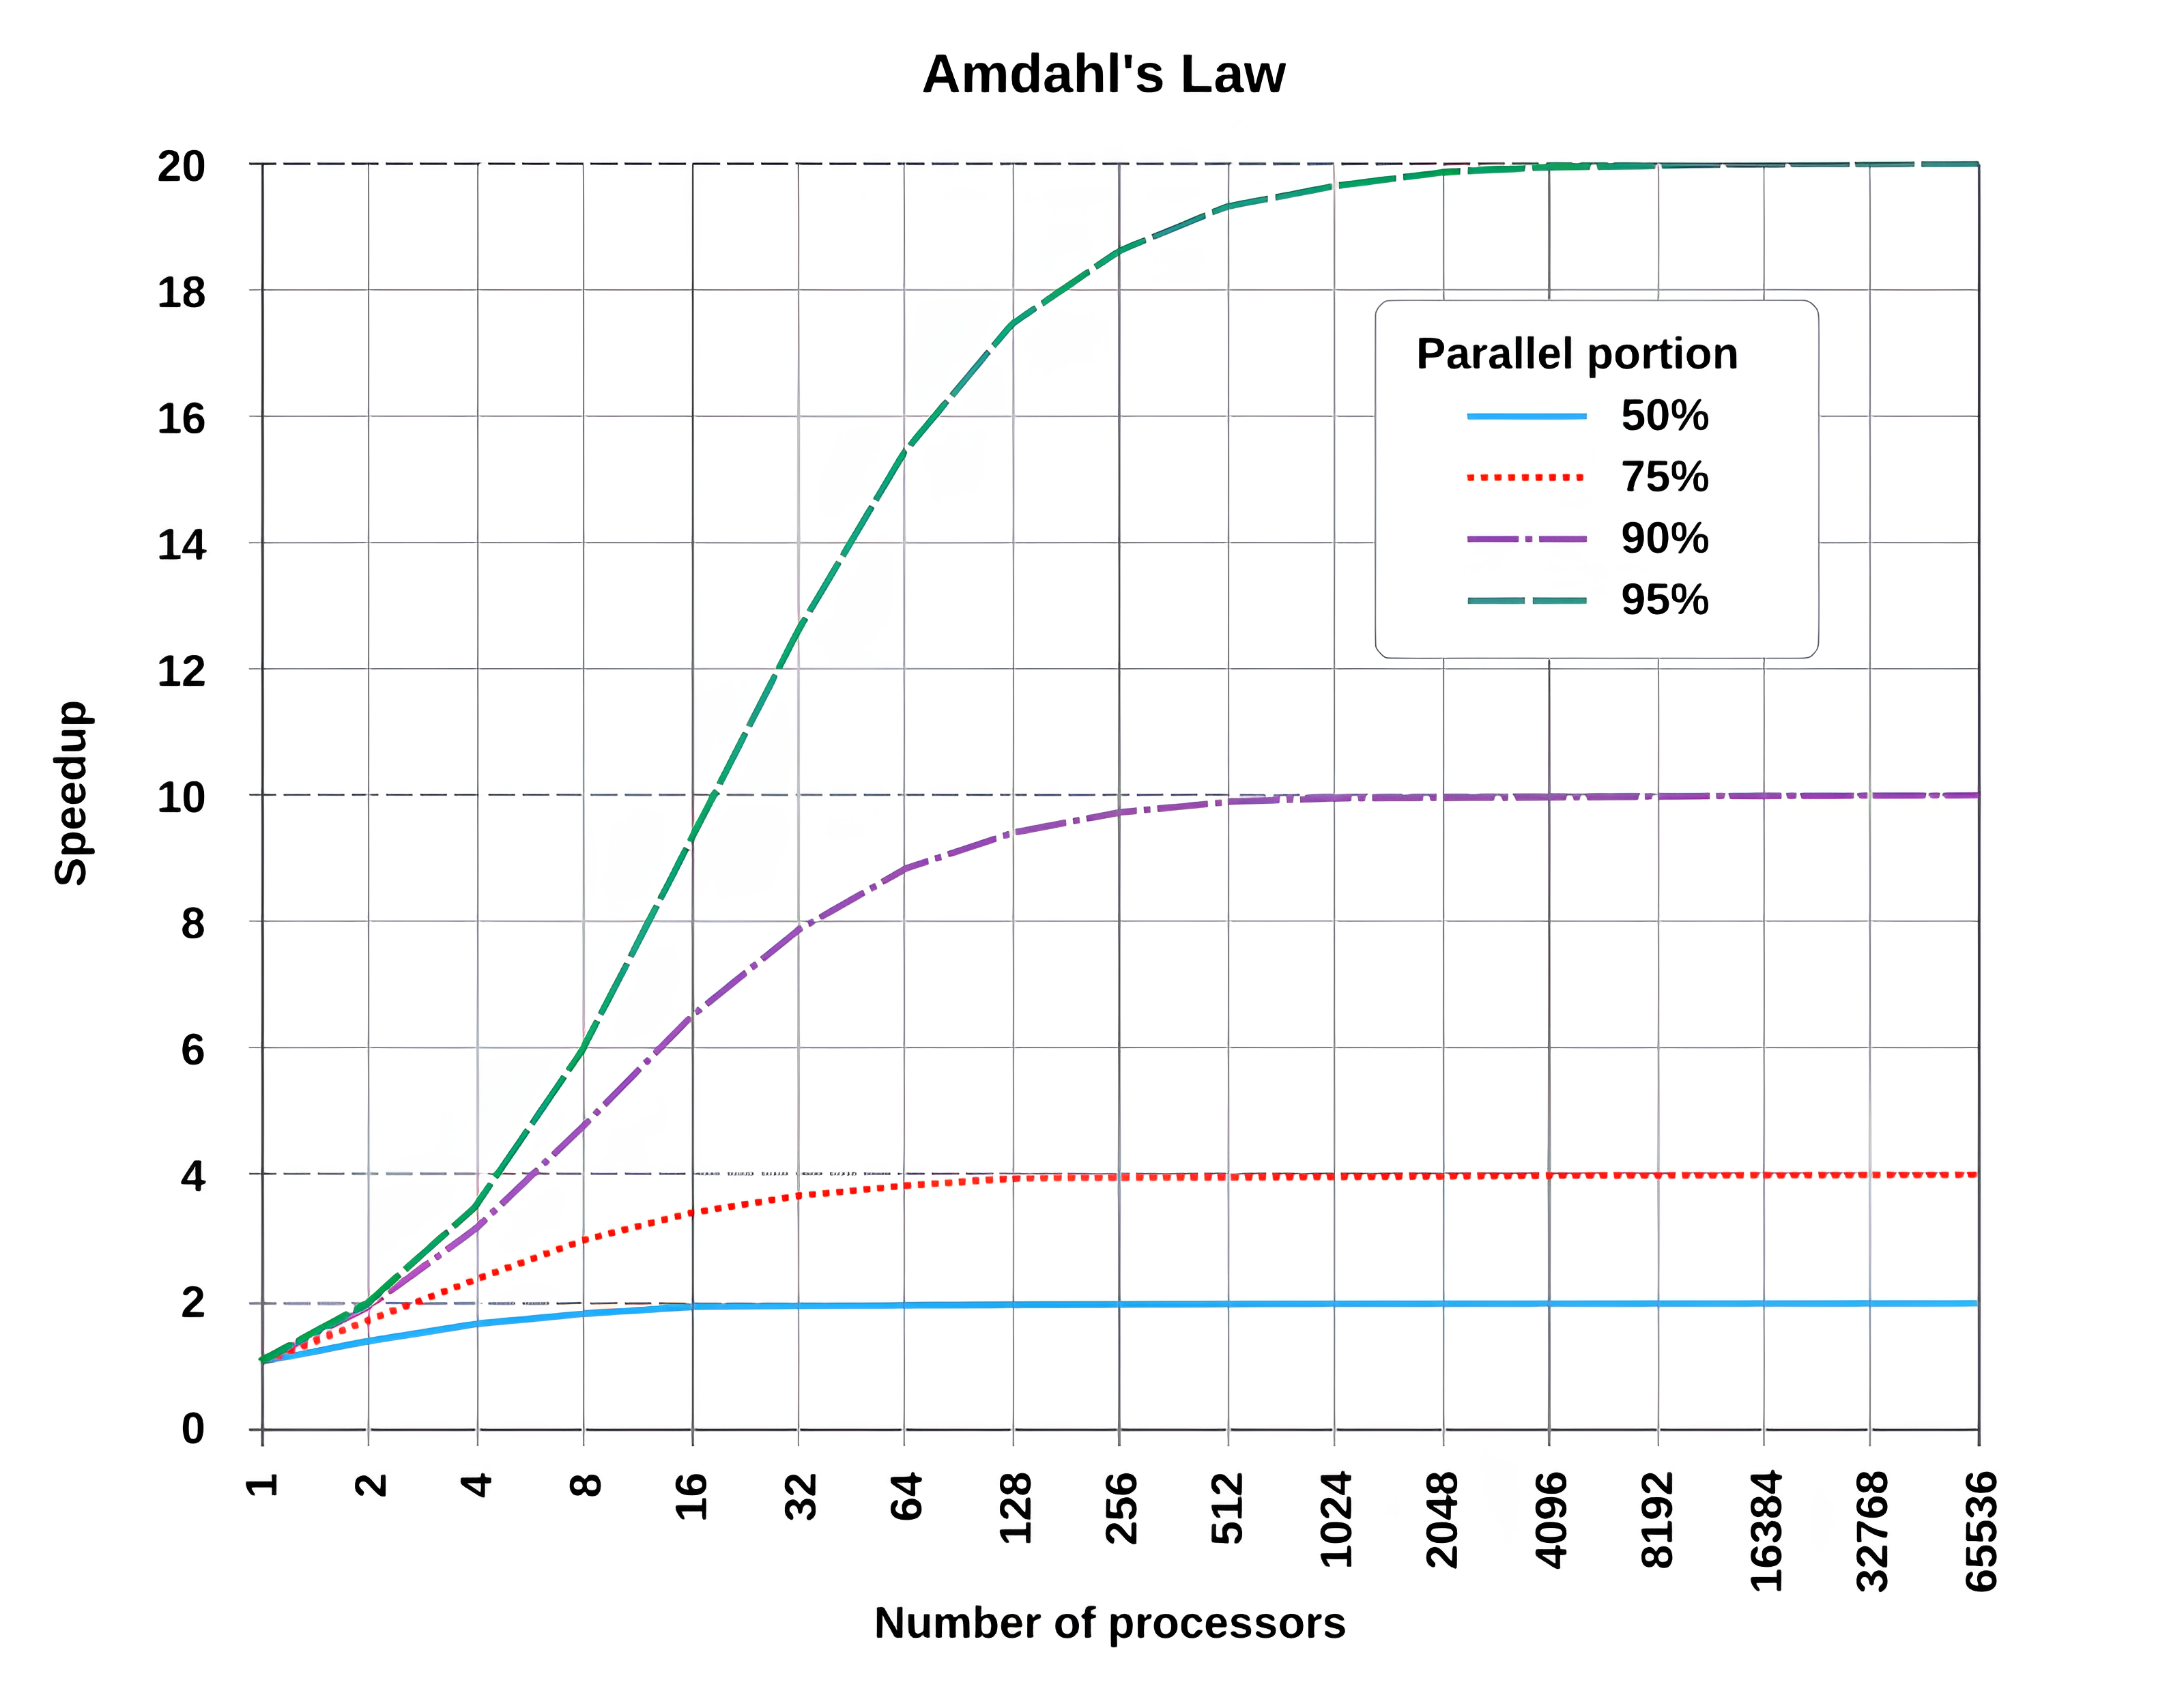
\includegraphics[width=0.7\textwidth]{images/Amdahls.png}
\end{center}
Questa legge non tiene conto del week scaling e decreta un comportamento ideale/approssimato. La \textbf{legge 
di Gustafson} tiene conto del week scaling 
$$ S(n,p)=(1-\alpha)+\alpha p$$
Nel caso reale, l'aumentare del numero di processi potrebbe far incrementare la frazione seriale.\begin{center}
    \includegraphics[width=0.7\textwidth]{images/speedUp.eps}
\end{center}
\flowerLine
\section{Operazioni su Vettori e Matrici}
\subsection{Scatter e Gather}
Consideriamo un algoritmo sequenziale che calcoli la somma di due vettori dati in input 
\begin{lstlisting}[style=CStyle]
void vector_sum(double x[], double y[], double z[], int n){
    for(int i=0; i<n; i++){
        z[i]=x[i]+y[i];
    }
}
\end{lstlisting}
Come si può distribuire tale compito su diversi processi? Si da l'assunzione che i vettori da 
sommare siano stati letti da standard input, quindi sono presenti nella memoria del processo con 
rank 0. Si vuole dividere il vettore equamente fra i diversi processi.\acc 
A tal proposito, esiste la funzione collettiva \code{int MPI\_Scatter}, che si occupa di prendere un 
vettore e di dividerlo equamente fra tutti i processi di un dato comunicatore.\begin{center}
    \includegraphics[width=0.4\textwidth]{images/scatter.eps}
\end{center}
I parametri della funzione sono i seguenti\begin{itemize}
    \item \code{void *send\_buf\_p} il buffer contenente il vettore da dividere
    \item  \code{int send\_count} il numero di elementi da inviare ad ogni processo, non il numero di elementi 
    totali del vettore
    \item  \code{MPI\_Datatype send\_type} il tipo degli elementi del vettore 
    \item  \code{void *recv\_buf\_p} il buffer che conterrà la frazione di vettore ricevuta, per il mittente, può 
    coincidere con il buffer di invio 
    \item  \code{int recv\_count} analogo a \codee{send\_count}
    \item  \code{MPI\_Datatype recv\_type} analogo a codee{send\_type}
    \item  \code{int src\_proc} il rank del processo che condividerà il vettore 
    \item \code{MPI\_Comm comm} il comunicatore in questione
\end{itemize}
La funzione assume che il numero di elementi da condividere sia divisibile per il numero di processi, l'ordine 
di condivisione avviene in base al rank. Il nodo che condivide il vettore può specificare la macro 
\code{MPI\_IN\_PLACE} come buffer di destinazione, e manterrà i valori nel vettore originale.\acc 
La funzione collettiva \code{int MPI\_Gather} è l'inversa della \code{scatter}, ogni nodo definisce un vettore, 
e ne verrà eseguita la concatenazione, per poi essere inviata ad un processo.\begin{center}
    \includegraphics[width=0.4\textwidth]{images/gather.eps}
\end{center}
L'ordine di concatenazione è sempre dato dal rank. I parametri sono pressocché identici alla \code{scatter}\begin{itemize}
    \item \code{void *send\_buf\_p} il buffer contenente il vettore parziale da inviare
    \item  \code{int send\_count} il numero di elementi contenuti nel vettore parziale
    \item  \code{MPI\_Datatype send\_type} il tipo degli elementi del vettore 
    \item  \code{void *recv\_buf\_p} il buffer che conterrà il vettore finale composta dalla concatenazione dei 
    vettori parziali 
    \item  \code{int recv\_count} analogo a \codee{send\_count}
    \item  \code{MPI\_Datatype recv\_type} analogo a codee{send\_type}
    \item  \code{int dest\_proc} il rank del processo che riceverà il vettore
    \item \code{MPI\_Comm comm} il comunicatore in questione
\end{itemize}
\textbf{Esempio di codice} : Il seguente programma, fa si che il processo di rank 0 generi 
due vettori con valori casuali, che verranno divisi fra i vari processi che eseguiranno delle somme parziali, 
trovando sezioni parziali del vettore somma, che verrà poi ri-unito con l'operazione collettiva.
\begin{lstlisting}[style=CStyle]
#include <stdio.h>
#include <stdlib.h>
#include <time.h>
#include <mpi.h>

void print_vector(int n, int *v, char name)
{
    printf("%c = [ ", name);
    for (int i = 0; i < n - 1; i++)
    {
        printf("%d, ", v[i]);
    }
    printf("%d ]\n", v[n - 1]);
}

int main(int argc, char **argv)
{
    MPI_Init(NULL, NULL);

    int my_rank;
    int size;
    int local_size = 3;
    MPI_Comm_size(MPI_COMM_WORLD, &size);

    int local_vector[size];
    int local_vector2[size];
    MPI_Comm_rank(MPI_COMM_WORLD, &my_rank);

    if (my_rank == 0)
    {

        int inputVector[local_size * size];
        int inputVector2[local_size * size];
        srand(time(NULL));
        for (int i = 0; i < local_size * size; i++)
        {
            inputVector[i] = rand() % 100;
            inputVector2[i] = rand() % 100;
        }
        print_vector(local_size * size, inputVector, 'A');
        print_vector(local_size * size, inputVector2, 'B');
        printf("\n");
        MPI_Scatter(inputVector, local_size, MPI_INT, local_vector, local_size,
                     MPI_INT, 0, MPI_COMM_WORLD);
        MPI_Scatter(inputVector2, local_size, MPI_INT, local_vector2, local_size,
                     MPI_INT, 0, MPI_COMM_WORLD);
    }
    else
    {
        MPI_Scatter(NULL, local_size, MPI_INT, local_vector, local_size,
                     MPI_INT, 0, MPI_COMM_WORLD);
        MPI_Scatter(NULL, local_size, MPI_INT, local_vector2, local_size,
                     MPI_INT, 0, MPI_COMM_WORLD);
    }
    printf("process %d :\n     A_%d = [ ", my_rank, my_rank);
    for (int i = 0; i < local_size - 1; i++)
    {
        printf("%d, ", local_vector[i]);
    }
    printf("%d ]\n     B_%d = [", local_vector[local_size - 1], my_rank);
    for (int i = 0; i < local_size - 1; i++)
    {
        printf("%d, ", local_vector2[i]);
    }
    printf("%d ]\n A_%d+B_%d = [", local_vector2[local_size - 1], my_rank, my_rank);
    for (int i = 0; i < local_size - 1; i++)
    {
        printf("%d, ", local_vector2[i] + local_vector[i]);
    }
    printf("%d ]\n\n", local_vector2[local_size - 1] + local_vector[local_size - 1]);

    int vec_sum[local_size];
    for (int i = 0; i < local_size; i++)
    {
        vec_sum[i] = local_vector2[i] + local_vector[i];
    }

    if (my_rank == 0)
    {
        int outVector[local_size * size];
        MPI_Gather(vec_sum, local_size, MPI_INT, outVector, local_size,
                    MPI_INT, 0, MPI_COMM_WORLD);
        print_vector(local_size * size, outVector, 'O');
    }
    else
    {
        MPI_Gather(vec_sum, local_size, MPI_INT, NULL, local_size,
                    MPI_INT, 0, MPI_COMM_WORLD);
    }

    MPI_Finalize();

    exit(0);
}
\end{lstlisting}
Le operazioni collettive sui vettori possono essere eseguite anche sulle matrici, anche se ciò dipende 
dall'allocazione di esse. Quando si dichiara una matrice di dimensioni 
statiche nel seguente modo \begin{quotation}
    \code{int matrix[n][n];}
\end{quotation}
essa viene allocata in maniera contigua in memoria.
\begin{center}
    \includegraphics[width=0.8\textwidth]{images/matrixDeclaration.eps}
\end{center}
In tal caso, le operazioni collettive di \textit{reduce} funzioneranno senza problemi dato che 
agiscono su blocchi di memoria contigui. Il punto è che una dichiarazione di questo tipo ha senso 
esclusivamente se è nota a priori la dimensione della matrice, nel caso più generale, una matrice 
si dichiara dinamicamente come un puntatore di puntatori di interi.
\begin{lstlisting}[style=CStyle]
int** a;
a = (int**) malloc(sizeof(int*)*num_rows);
for(int i = 0; i < num_rows; i++){
    a[i] = (int*) malloc(sizeof(int)*num_cols);
}
\end{lstlisting}
Le righe della matrice in questo caso \textit{non} sono contigue in memoria, non è quindi possibile 
utilizzare operazioni di \textit{reduce}, per far ciò, bisogna collassare la matrice in un 
array bidimensionale regolando l'accesso degli indici. Su una matrice statica, l'accesso avviene 
per mezzo di due indici \code{matrix[i][j]}, se la matrice è collassata in un 
array, un solo indice deve codificare entrambi gli indici della matrice, nella pratica, si fa così\begin{quote}
    \code{matrix[i*num\_col+j]}
\end{quote}
Una matrice allocata dinamicamente come un unico array può essere soggetta alle operazioni di \textit{reduce}.
\begin{center}
    \includegraphics[width=0.8\textwidth]{images/matrixDeclaration2.eps}
\end{center}
\subsubsection{Prodotto fra Vettori e Matrici}
Come visto nel corso di 
\color{blue}\href{https://github.com/CasuFrost/University_notes/blob/main/Secondo%20Anno/Primo%20Semestre/Algebra/Latex%20source%20file/Algebra.pdf}{Algebra}\color{black}, 
il prodotto scalare fra due vettori è definito come segue 
$$ \begin{bmatrix}
    a_1&a_2&\dots&a_n
\end{bmatrix}\cdot \begin{bmatrix}
    b_1\\b_2\\\dots\\b_n
\end{bmatrix}=a_1\cdot b_1 + a_2\cdot b_2+\dots + a_n\cdot b_n$$
Il prodotto fra una matrice $n\times n$ ed un vettore $\bar b$ di $n$ componenti, è un vettore sempre di 
$n$ componenti, di cui ogni $i$-esimo componente è il prodotto scalare fra la $i$-esima riga della matrice 
ed il vettore $\bar b$. 
$$ \begin{bmatrix}
    a_{1_1}&a_{1_2}&\dots&a_{1_n}\\ 
    a_{2_1}&a_{2_2}&\dots&a_{2_n}\\ 
    \vdots & \vdots &\ddots & \vdots\\ 
    a_{n_1}&a_{n_2}&\dots&a_{n_n}
\end{bmatrix}\cdot \begin{bmatrix}
    b_1\\b_2\\\dots\\b_n
\end{bmatrix}=\begin{bmatrix}
    a_{1_1}b_1+a_{1_2}b_2+\dots+a_{1_n}b_n\\
    a_{2_1}b_1+a_{2_2}b_2+\dots+a_{2_n}b_n\\
    \vdots\\
    a_{n_1}b_1+a_{n_2}b_2+\dots+a_{n_n}b_n
\end{bmatrix}$$
\begin{lstlisting}[style=CStyle]
int A[n][n]; //matrice 
int b[n]; //vettore input
int y[n]; //vettore risultato
for(i=0;i<n;i++){
    for(j=0;j<n;j++){
        y[i]=A[i][j]*b[j] //prodotto scalare implicitamente definito
    }
}
\end{lstlisting}
\subsection{Ultime Collettive di tipo "All"}
La collettiva \code{int MPI\_Allgather} si occupa di 
unire i dati di un vettore come la normale funzione di 
\textit{gather}, per poi condividere i dati con tutti i 
processi di un comunicatore, logicamente, equivale ad una 
gather seguita da una broadcast, ma è implementata in 
maniera più efficiente.
\begin{center}
    \includegraphics[width=0.3\textwidth]{images/allgather.eps}
\end{center}\begin{itemize}
    \item     \code{void *send\_buf\_p}
    \item     \code{int send\_count}
    \item     \code{MPI\_Datatype send\_type}
    \item     \code{int recv\_count}
    \item     \code{MPI\_Datatype recv\_type}
    \item     \code{MPI\_Comm comm}
\end{itemize}
La collettiva \code{MPI\_Allscatter} equivale ad una 
reduce seguita da una scatter.
$$ 
\begin{bmatrix}
    a_1 \\ a_2 \\ \vdots\\ a_n
\end{bmatrix} \ \ 
\begin{bmatrix}
    b_1 \\ b_2 \\ \vdots\\  b_n
\end{bmatrix}\ \ 
\begin{bmatrix}
    c_1 \\ c_2 \\ \vdots\\  c_n
\end{bmatrix} =\text{Allscatter}\Rightarrow
\begin{bmatrix}
    a_1+b_1+c_1 \\ 0\\ \vdots\\ 0
\end{bmatrix} \ \ 
\begin{bmatrix}
    0 \\ a_2+b_2+c_2 \\ \vdots\\  0
\end{bmatrix}\ \ 
\begin{bmatrix}
    0 \\ 0 \\ \vdots\\  a_n+b_n+c_n
\end{bmatrix} 
$$\flowerLine
\section{Tipi di Dato Custom}
Abbiamo visto come MPI implementi il tipo 
\code{MPI\_Datatype} per riferirsi ai tipi di dato presenti 
nel C. In C, è però possibile creare dei tipi di dato 
aggiuntivi (struct).
\begin{lstlisting}[style=CStyle]
struct t{
    float a,
    float b,
    int n
};
\end{lstlisting}
Cosa va definito nel capo \code{data\_type} quando si 
intente inviare tramite una funzione MPI una struttura? 
MPI permette di creare dei tipi custom, è possibili 
definire \textbf{tipi derivati}, che equivalgano (in quanto 
disposizione in memoria) alla struct in questione. Un tipo 
derivato non è altro che una sequenza di 
datatype di base alla quale è assengata una certa 
disposizione in memoria. \begin{quote}
    \code{{(MPI\_DOUBLE,0), (MPI\_DOUBLE,16),(MPI\_INT,24)}}
\end{quote}
Un tipo derivato va definito tramite la funzione 
\code{int MPI\_Type\_create\_struct}:\begin{itemize}
    \item \code{int count} il numero di elementi distinti nel tipo derivato 
    \item \code{int array\_of\_blocklengths[]} ogni elemento potrebbe essere un vettore, va 
    quindi specificata la lunghezza di ogni elemento della struct.
    \item \code{MPI\_Aint array\_of\_displacements} la disposizione degli elementi della 
    struct in memoria 
    \item \code{MPI\_Datatype *new\_type\_p} il tipo degli elementi della nuova struttura  
\end{itemize}
Per ottenere la disposizione è possibile usare il puntatore del valore,  
è pero auspicabile utilizzare la funzione di liberia 
\code{MPI\_Get\_address}, in quanto in alcuni sistemi (seppur pochi) i puntatori potrebbero 
non rappresentare un indirizzo di memoria.
\begin{lstlisting}[style=CStyle]
MPI\_Aint a_addr, b_addr, n_addr;
MPI_Get_address(&a, &a_addr);
array_of_displacements[0]=0;
MPI_Get_address(&b, &b_addr);
array_of_displacements[1]=b_addr-a_addr;
MPI_Get_address(&n, &n_addr);
array_of_displacements[2]=n_addr-a_addr;
\end{lstlisting}
Una volta creata tale struttura, bisogna eseguire 
la funzione \code{MPI\_Type\_commit} che, eseguendo opportune ottimizzazioni,
 decide il metodo di salvataggio della struttura in memoria. 
 Quando non è più necessario quel datatype,
  si può chiamare la funzione \code{MPI\_Type\_free}.
\chapter{Memoria Condivisa : Posix Threads}
\section{Introduzione ai Thread}
In MPI, un insieme di nodi comunica tramite lo scambio di messaggi su un apposito canale, all'interno di ogni 
nodo, sono presenti delle unità di calcolo con più cores, ossia più sotto-unità che comunicano ed operano 
contemporaneamente su una memoria condivisa.\acc 
Se MPI si occupa della comunicazione fra più nodi, è necessario un paradigma volto alla comunicazione dei differenti core 
di un'unità di calcolo che possono accedere ad una memoria comune. \acc 
Un processo è un istanza di un programma (in esecuzione) che viene caricata sulla CPU, possiamo identificare 
i \textit{singoli flussi indipendenti di computazione} di un processo, denominati \textbf{thread}, 
analoghi ai processi ma più "leggeri" nella loro creazione e gestione, due thread appartenenti ad uno 
stesso processo hanno differenti program counter e stack ma condividono lo stesso spazio di indirizzamento 
dinamic (heap), la comunicazione è semplice, in quanto basta scrivere sulla stessa area di memoria.\begin{center}
    \includegraphics[width=0.8\textwidth]{images/thread..eps}
\end{center} 
Lo standard \textbf{Posix Threads (Pthreads)} è implementato con una libreria in C e specifica l'API per 
l'interazione fra i thread, è necessario specificare nel codice la direttiva di inclusione\begin{quote}
    \code{\# include <pthread.h>}
\end{quote}
La libreria fornisce il tipo di dato \code{pthread\_t}, non è importante la sua struttura interna, basti 
sapere che tale tipo identifica univocamente un thread all'interno di un processo, a volte viene 
denotato \textit{thread handler}. La creazione di un thread avviene tramite la chiamata di libreria
\code{int pthread\_create}, i cui parametri sono\begin{itemize}
    \item \code{pthread\_t* thread\_p} verrà assegnato l'identificatore del thread creato. 
    \item \code{const pthread\_attr\_t* attr\_p} attributi in input che per adesso verranno ignorati. 
    \item \code{void* (*start\_routine ) ( void* )} la funzione che verrà eseguita dal thread creato. 
    \item \code{void* arg\_p} i parametri della funzione sopracitata.
\end{itemize}
All'avvio di un thread è quindi necessario specificarne la funzione da eseguire, una funzione può 
essere passata in input in quanto rappresenta un puntatore alla zona di memoria in cui è contenuta 
la procedura da eseguire.
\begin{lstlisting}[style=CStyle]
void func(int a){
    /*codice*/
}

void(*func_ptr)(int)=func; /*puntatore a funzione in cui se ne specifica anche il tipo 
                           [int] del parametro*/
\end{lstlisting}
Convenzionalmente, la funzione del thread è di tipo puntatore a void e ha come parametro di ingresso 
un puntatore a void (caso più generale possibile) che verrà eventualmente castato.\begin{quote}
    \code{void *thread\_function(void *args\_p);}
\end{quote}
Per attendere la terminazione di un thread da parte del processo principale è necessario utilizzare 
la funzione \code{pthread\_join}, valida per un singolo thread, i parametri sono\begin{itemize}
    \item \code{pthread\_t thread} l'identificatore del thread di cui attendere la terminazione 
    \item \code{void **value\_ptr} il valore di ritorno del thread
\end{itemize}
La funzione \code{pthread\_self} ritorna l'identificatore del thread chiamante. Il seguente esempio mostra 
la creazione di diversi thread che stampano a schermo una stringa.
\begin{lstlisting}[style=CStyle]
    #include <stdio.h>
    #include <stdlib.h>
    #include <pthread.h>
    #define THREAD_COUNT 4
    
    void *Hello(void *rank)
    {
        int my_rank = rank;
        printf("hello from thread %ld\n", my_rank);
        return NULL;
    }
    
    int main()
    {
        pthread_t thread_handles[THREAD_COUNT];
        for (int i = 0; i < THREAD_COUNT; i++) /*creazione dei thread*/
            pthread_create(&thread_handles[i], NULL, Hello, (void *)i);
        printf("hello from main thread\n");
        for (int i = 0; i < THREAD_COUNT; i++) /*terminazione dei thread*/
            pthread_join(thread_handles[i], NULL);
        return 0;
    }
\end{lstlisting}
Riguardo il numero dei thread, sarebbe corretto considerare tanti thread quanti sono i core fisici sulla 
macchina che esegue il programma. Se si vogliono passare \textit{molteplici} parametri ad un thread è necessario 
definire un'apposita struct che li comprenda.
\subsection{Prodotto Matrice-Vettore con Pthread}
Si vuole eseguire il calssico algoritmo di moltiplicazione di una matrice per un vettore, la cui 
computazione seriale si ricorda essere
\begin{lstlisting}[style=CStyle]
/* m := righe di A*/
/* n := elementi di di x*/
/* y := vettore output*/
for(int i = 0;i<m;i++){
    y[i]=0.0;
    for(int j=0;j<n;j++){
        y[i]+=A[i][j]*x[j];
    }
}
\end{lstlisting}
Si vuole parallelizzare l'esecuzione fra più thread, come prima cosa, si supponga di avere tanti thread 
quante sono le righe della matrice in input (quindi, gli elementi del vettore in output), e di far calcolare 
ad ogni thread $i$ il valore dell'$i$-esimo elemento del vettore in output.\begin{center}
    \includegraphics[width=0.5\textwidth]{images/threadMatProd.eps}
\end{center} 
In generale, se il numero di thread è $t<m$, ogni $q$-esimo thread computerà $\frac{m}{t}$ righe, ossia dalle \begin{itemize}
    \item \color{teal}$q\cdot\nicefrac{m}{t}$\color{black}-esima riga 
    \item alla \color{teal}$(q+1)\nicefrac{m}{t}-1$\color{black}-esima riga
\end{itemize}
Si ha il seguente codice
\begin{lstlisting}[style=CStyle]
    #include <stdio.h>
    #include <stdlib.h>
    #include <pthread.h>
    
    #define MAT_ORDER 6
    #define THREAD_COUNT 6
    
    /*Siano A la matrice, x il vettore in input ed y il vettore in output*/
    
    void *mat_vec_product(void *rank)
    {
        int my_rank = rank;
        int local_m = MAT_ORDER / THREAD_COUNT;
        int first_row = my_rank * local_m;
        int last_row = ((my_rank + 1) * local_m) - 1;
    
        for (int i = first_row; i <= last_row; i++)
        {
            y[i] = 0;
    
            for (int j = 0; j < MAT_ORDER; j++)
            {
                y[i] += A[i][j] * x[j];
            }
        }
    }
    
    int main()
    {
        pthread_t handler[THREAD_COUNT];
        for (int i = 0; i < THREAD_COUNT; i++)
            pthread_create(&handler[i], NULL, mat_vec_product, (void *)i);
        for (int i = 0; i < THREAD_COUNT; i++)
            pthread_join(handler[i], NULL);
        return 0;
    }
\end{lstlisting}\flowerLine 
\section{Sezioni Critiche}
Si consideri il seguente scenario : Vi è una variabile (intera) \texttt{x} inizializzata a 0 
 condivisa da due thread, 
entrambi si adoperano per incrementare la variabile di 1, ci si aspetta, che dopo l'esecuzione la 
variabile \texttt{x} sia uguale a 2. Il punto è che l'incremento di una variabile (somma) in C, equivale ad 
una sequenza di istruzioni assembly che possono essere intergogliate dai due thread.\begin{center}
    \begin{tabular}{ccc}
        \hline
        \multicolumn{1}{|c|}{\cellcolor[HTML]{EFEFEF}istanti di tempo} & \multicolumn{1}{c|}{\cellcolor[HTML]{ECF4FF}thread 0}                                                                                                             & \multicolumn{1}{c|}{\cellcolor[HTML]{FFFFC7}thread 1}                                                                                                             \\ \hline
        \multicolumn{1}{l}{}                                           & \multicolumn{1}{l}{}                                                                                                                                              & \multicolumn{1}{l}{}                                                                                                                                              \\ \hline
        \multicolumn{1}{|c|}{1}                                        & \multicolumn{1}{c|}{\begin{tabular}[c]{@{}c@{}}inizalizzato dal \\ main thread\end{tabular}}                                                                      & \multicolumn{1}{c|}{}                                                                                                                                             \\ \hline
        \multicolumn{1}{|c|}{2}                                        & \multicolumn{1}{c|}{\begin{tabular}[c]{@{}c@{}}legge la variabile \texttt{x=0}\\ e la carica nel registro r1\end{tabular}}                       & \multicolumn{1}{c|}{\begin{tabular}[c]{@{}c@{}}inizalizzato dal \\ main thread\end{tabular}}                                                                      \\ \hline
        \multicolumn{1}{|c|}{3}                                        & \multicolumn{1}{c|}{\begin{tabular}[c]{@{}c@{}}incrementa il registro r1=0  di 1, \\ avendo r1=1\end{tabular}}                                                    & \multicolumn{1}{c|}{\begin{tabular}[c]{@{}c@{}}legge la variabile \texttt{x=0}\\ e la carica nel registro r2\end{tabular}}                       \\ \hline
        \multicolumn{1}{|c|}{4}                                        & \multicolumn{1}{c|}{\begin{tabular}[c]{@{}c@{}}salva il valore del registro in \texttt{x}, \\ si ha  \texttt{x=1}\end{tabular}} & \multicolumn{1}{c|}{\begin{tabular}[c]{@{}c@{}}incrementa il registro r2=0  di 1, \\ avendo r2=1\end{tabular}}                                                    \\ \hline
        \multicolumn{1}{|c|}{5}                                        & \multicolumn{1}{c|}{termina}                                                                                                                                      & \multicolumn{1}{c|}{\begin{tabular}[c]{@{}c@{}}salva il valore del registro in \texttt{x}, \\ si ha  \texttt{x=1}\end{tabular}} \\ \hline
        \multicolumn{1}{|c|}{6}                                        & \multicolumn{1}{c|}{}                                                                                                                                             & \multicolumn{1}{c|}{termina}                                                                                                                                      \\ \hline
        \end{tabular}
\end{center}
Alla fine dell'esecuzione la variabile \texttt{x} sarà uguale ad 1 perché i due thread non si sono 
sincronizzati correttamente. Tale problema è noto come \textbf{race condition} e ha comportato la nascita di 
una vasta teoria riguardante la sincronizzazione dei processi paralleli che accedono a risorse condivise, in questa sezione 
verranno presentate delle possibili soluzioni.
\subsection{Busy Waiting e Mutex}
Il tema centrale è la mutua esclusività delle variabili, l'accesso ad esse non può venire contemporaneamente da parte 
di più thread, con \textbf{busy waiting}, si denota una metodologia che consiste nel far attendere un processo che tenta 
di accedere ad una variabile già in uso, lasciandolo bloccato in un ciclo in cui ad ogni iterazione 
controlla la disponibilità della risorsa.\acc 
Nel seguente esempio, ogni thread viene bloccato in un ciclo finché la variabile \code{flag} non 
diventa uguale al loro rank. A seguito dell'utilizzo dovranno incrementare la variabile per permettere 
al prossimo thread di accedere.
\begin{lstlisting}[style=CStyle]
    while(flag!=my_rank);
    x+=1;
    flag++;
\end{lstlisting}
Il busy waiting, seppur semplice nella sua implementazione, comporta svantaggi difficilmente trascurabili\begin{itemize}
    \item un processo in attesa occuperà inutilmente la CPU comportando uno spreco di computazione 
    \item Il compilatore, se nota un indipendenza apparente fra due istruzioni, potrebbe invertirne l'ordine, ad esempio, 
    trasformando il codice come segue
\end{itemize}
\begin{lstlisting}[style=CStyle]
    x+=1;
    while(flag!=my_rank); /* sequenza di istruzioni errata */
    flag++;
\end{lstlisting}
Tale riarrangiamento è parte di una serie di ottimizzazioni che fa il compilatore. Disattivare tali ottimizzazioni 
comporterebbe un uso meno efficiente dei registri per tutte le altre istruzioni.\acc 
Le \textbf{Mutex} permettono una gestione più sofisticata degli accessi alle risorse mutualmente 
esclusive, una Mutex è una variabile utilizzata per restringere l'accesso ad una risorsa, per poi 
rilasciarla una volta utilizzata.\acc 
Una mutex viene gestita dal tipo di dato \code{pthread\_mutex\_t}, una volta definita, va inizializzata 
tramite la funzione \code{int pthread\_mutex\_init}, 
assegnandole la variabile il cui accesso deve essere regolamentato. La funzione ha i seguenti 
parametri\begin{itemize}
    \item \code{pthread\_mutex\_t *mutex\_p} la mutex a cui si riferisce 
    \item \code{const pthread\_mutexattr\_t *attr\_p} degli attributi che per adesso saranno ignorati.
\end{itemize}
Quando si vuole accedere ad una variabile protetta da una mutex bisogna controllarne lo stato, che può 
essere \textit{bloccato} o \textit{libero}. Si richiede l'accesso alla variabile tramite la chiamata 
\begin{quote}
    \code{int pthread\_mutex\_lock(pthread\_mutex\_t *mutex\_p)}
\end{quote} 
Se l'accesso è libero, il thread continuerà la sua esecuzione, altrimenti verrà \textit{sospeso} (senza 
occupare tempo sulla CPU), e potrà continuare la sua esecuzione solo quando la lock sarà rilasciata.\acc 
Una volta che un thread ha terminato l'accesso alla variabile, deve rilasciare la lock con la chiamata 
\begin{quote}
    \code{int pthread\_mutex\_unlock(pthread\_mutex\_t *mutex\_p)}
\end{quote} 
Una volta terminata l'utilità di una mutex, va eliminata con la chiamata \begin{quote}
    \code{int pthread\_mutex\_destroy(pthread\_mutex\_t *mutex\_p)}
\end{quote}
Il fenomeno della \textbf{Starvation} si verifica quando l'esecuzione di un thread o di un
 processo viene sospesa o impedita per un tempo indefinito, anche se è in grado di continuare 
 l'esecuzione. È tipicamente associata all'imposizione di priorità o alla mancanza di equità nella 
 pianificazione o nell'accesso alle risorse.
Se una mutex è bloccata, il thread viene bloccato e inserito in una coda di thread in attesa. Se la coda è FIFO, non si verificherà starvation.
\acc 
Un \textbf{Deadlock} invece identifica una situazione di attesa circolare in cui ogni elemento di un insieme 
di thread è sia in attesa del rilascio di una lock, sia in possesso di una lock necessaria agli altri thread. 
\begin{center}
	\begin{tabular}{>{\centering\arraybackslash}m{3in}>{\arraybackslash}m{3in}}
    \begin{lstlisting}[style=CStyle]
            pthread_mutex_lock(&a); 
            pthread_mutex_unlock(&b);
            /*in attesa di a per 
            rilasciare b*/
        \end{lstlisting}&
        \begin{lstlisting}[style=CStyle]
            pthread_mutex_lock(&b); 
            pthread_mutex_unlock(&a);
            /*in attesa di b per 
            rilasciare a*/
        \end{lstlisting}
	\end{tabular}
\end{center}
In termini di prestazioni il Mutex mostra performance più elevate rispetto il busy 
waiting quando il numero di thread 
è superiore al numero di core fisici, si osservi la seguente tabella che riporta i tempi 
impiegati (in secondi) per stimare il valore di $\pi$ su una macchiana con 8 core.\begin{center}
    \begin{tabular}{c|c|c}
        \rowcolor[HTML]{FFFFC7} 
        num. thread & busy waiting & mutex \\ \hline
        \rowcolor[HTML]{ECF4FF} 
        1           & 2.9          & 2.9   \\
        \rowcolor[HTML]{EFEFEF} 
        2           & 1.45         & 1.45  \\
        \rowcolor[HTML]{ECF4FF} 
        4           & 0.73         & 0.73  \\
        \rowcolor[HTML]{EFEFEF} 
        8           & 0.38         & 0.38  \\
        \rowcolor[HTML]{ECF4FF} 
        16          & 0.5          & 0.38  \\
        \rowcolor[HTML]{EFEFEF} 
        32          & 0.8          & 0.4   \\
        \rowcolor[HTML]{ECF4FF} 
        64          & 3.56         & 0.38 
        \end{tabular}
\end{center}
\subsection{Semafori, Barriere e Variabili di Condizione}
Il busy waiting permette l'accesso esclusivo ai thread imponendo anche un certo ordine, ma presenta 
degli svantaggi considerevoli, che però non presenta l'utilizzo delle mutex, seppur quest'ultimo 
lascia l'ordine di accesso indeterminatoe deciso dal sistema operativo, ci sono situazioni in cui 
si vuole un accesso ordinato senza dover subire i problemi del busy waiting.\acc 
Lo standard Posix definisce un costrutto simile al mutex ma più elaborato : i \textbf{Semafori}, che rappresentano 
delle mutex \textit{non binarie}. Per utilizzarli, si include la direttiva\begin{quotation}
    \code{\# include <semaphore.h>}
\end{quotation}
L'handler dei semafori è il tipo \code{sem\_t}, un semaforo viene inizializzato con \code{int sem\_init} i cui 
parametri sono\begin{itemize}
    \item \code{sem\_t* semaphore\_p}
    \item \code{int shared} se uguale ad 1, sarà condiviso anche fra diversi processi 
    \item \code{unsigned initial\_val} il numero intero con il quale è inizializzato un semaforo
\end{itemize}
Il funzionamento è il seguente, quando un thread vuole accedere ad una sezione, chiama la funzione 
\code{sem\_wait(sem\_t *sem)}, ad ogni semaforo è associato un numero intero, se tale numero è maggiore 
di zero al momento della chiamata, il processo potrà procedere, e decrementerà di 1 il valore del semaforo. \acc 
Se il valore è uguale a zero, il processo si arresterà entrando in una 
coda di attesa, attendendo il via libera per ripartire.\acc 
Quando un thread termina con l'utilizzo del semaforo, può chiamare la funzione \code{sem\_post(sem\_t * sem)} che 
farà procedere un thread in attesa del semaforo nell'esecuzione. Se la coda è vuota, il valore del semaforo verrà incrementato 
di 1.\begin{center}
    \includegraphics[width=1\textwidth]{images/sem.eps}
\end{center}
Con \textbf{barriera} si intende un costrutto che viene inserito in un certo punto del codice, in cui 
ogni thread che lo esegue, per poter continuare l'esecuzione oltre tale punto deve attendere che ogni altro thread 
vi sia arrivato, serve a risincronizzare l'esecuzione dei thread facendoli ripartire da un punto comune. Un tipico esempio 
può essere quello di voler far noto in fase di debug che tutti thread hanno raggiunto un certo punto 
del codice.
\begin{lstlisting}[style=CStyle]
    /*punto comune del programma*/
    barriera;
    if(my_rank==0){
        printf("tutti i thread hanno raggiunto questo punto \n");
        fflush(stdout);
    }
\end{lstlisting}
L'implementazione di una barriera tramite l'uso del busy waiting e delle mutex è intiuitiva, 
si utilizza un contatore condiviso inizializzato a zero (il cui accesso è protetto da mutex) e si incrementa di 1 
per ogni thread che arriva a tal punto. Ogni thread sarà in busy waiting finché il contatore non sarà uguale al 
numero dei thread.
\begin{lstlisting}[style=CStyle]
    int counter = 0;
    int thread_number;
    pthread_mutex barrier_mutex;

    void *thread_function(void *arg_p){
        ...
        /*implementazione della barriera*/
        pthread_mutex_lock(&barrier_mutex);
        counter++;
        pthread_mutex_unlock(&barrier_mutex);
        while(counter<thread_number);
        /*fine della barriera*/
        ...
    }
\end{lstlisting}
Una barriera può anche essere implementata con un semaforo. L'implementazione mostrata presenta un problema, 
se fosse necessario riutilizzare tale barriera, bisognerebbe resettare la variabile \code{counter} a 
zero. Tale reset però deve avvenire solo \textit{in seguito} al passaggio di tutti i thread 
della barriera, potrebbe capitare che un thread non si sia reso conto che la variabile counter 
avesse raggiunto il valore sufficiente per proseguire, rimanendo bloccato nella barriera. Questo problema, 
nonostante possa sembrare banale, è in realtà un intralcio considerevole e non ha soluzioni immediate.\acc 
Può essere di aiuto l'uso di una \textbf{variabile di condizione}, queste ultime sono un \textit{oggetto} 
associato ad una mutex, che permettono ad un thread di sospendere la sua esecuzione fino all'accadere di un 
determinato \textit{evento}, si definiscono con il tipo 
\code{pthread\_cond\_t}. A seguito di tale evento, il thread può essere svegliato con un apposito 
segnale. Una variabile di condizione descrive un \textit{evento}.
\begin{center}
    \begin{lstlisting}[style=CStyle]
    lock mutex;
    if CONDIZIONE SI AVVERA : /* avvisa i thread che la condizione si e' avverata*/
        signal thread(s); 
    else : /*se non e' verificata, si libera la lock e si attende la condizione*/
        unlock mutex
        SOSPENSIONE ESECUZIONE 
    unlock mutex;
    \end{lstlisting}
\end{center}
In seguito, l'implementazione di una barriera con delle variabili di condizione.
\begin{lstlisting}[style=CStyle]
    int counter = 0; /*variabile condivisa*/
    pthread_mutex_t mutex;
    pthread_cond_t cond_var;
    ... 

    void *thread\_function(void *args_p){
        ... 
        /*barriera*/
        ptrhead_mutex_lock(&mutex);
        counter++;
        if(counter==thread_count){
            counter=0;
            pthread_cond_broadcast(&cond_var); /*avvisa tutti i thread che 
                                                 la condizione si e' avverata*/
        }else{
            while(pthread_cond_wait(&cond_var,&mutex)!=0); 
        }
        ptrhead_mutex_unlock(&mutex);
    }
\end{lstlisting}
Si osservi la riga di codice 16\begin{quote}
    \code{while(pthread\_cond\_wait(\&cond\_var,\&mutex)!=0); }
\end{quote}
La chiamata \code{pthread\_cond\_wait} sospende il processo, perché allora è necessario inserirla 
all'interno di un while come se andasse verificato periodicamente? È buona norma dato che il sistema operativo 
potrebbe inaspettatamente svegliare un processo dallo stato di attesa prima che la condizione si avveri, queste 
\textit{sveglie spurie} vanno quindi gestite.\begin{itemize}
    \item \code{pthread\_cond\_signal(pthread\_cond\_t* cond\_var\_p);} sveglia un thread in attesa
    \item \code{pthread\_cond\_broadcast(pthread\_cond\_t* cond\_var\_p);} sveglia tutti i thread in attesa
    \item \code{pthread\_cond\_init(pthread\_cond\_t*  cond\_p, \\ 
    pthread\_condattr\_t* cond\_attr\_p)} inizializza una variabile di condizione
    \item \code{pthread\_cond\_destroy(pthread\_cond\_t*  cond\_p)} termina una variabile di condizione
    \item La funzione\begin{quote}
        \code{pthread\_cond\_wait(pthread\_cont\_t* cond\_var\_p, 
        pthread\_mutex\_t mutex\_p)}
    \end{quote} si occupa di \begin{enumerate}
        \item   fare l'unlock della mutex 
        \item   sospendere il thread finché non arriva un segnale di risveglio  
        \item fare la lock della mutex una volta svegliato il thread
    \end{enumerate}
\end{itemize}

\newpage \subsection{Stima di $\pi$ con Pthread}
\begin{lstlisting}[style=CStyle]
#include <stdio.h>
#include <stdlib.h>
#include <pthread.h>
#include <time.h>

unsigned precision = 100000; /*punti generati da ogni thread*/
const unsigned thread_number = 6;

unsigned total_tosses;
unsigned point_in_center = 0;

/*gestione accesso a variabili condivise*/
pthread_mutex_t mutex;

void *thread_function(void *arg_p)
{
    int local_circle_point = 0;

    for (int i = 0; i <= precision; i++)
    {
        double x = (double)rand() / RAND_MAX * 2.0 - 1.0; /*Generazione punto casuale*/
        double y = (double)rand() / RAND_MAX * 2.0 - 1.0;
        local_circle_point += (x * x + y * y < 1); /*Controllo se e' nel cerchio*/
    }

    /*L'accesso alla variabile condivisa deve essere mutualmente esclusivo*/
    pthread_mutex_lock(&mutex);
    point_in_center += local_circle_point;
    pthread_mutex_unlock(&mutex);
}

int main(int argc, char **argv)
{
    srand(time(NULL));

    if (argc > 1)
    {
        precision = atoi(argv[1]);
    }

    total_tosses = precision * thread_number;
    pthread_mutex_init(&mutex, NULL);
    pthread_t tids[thread_number];

    for (int i = 0; i < thread_number; i++)
    {
        pthread_create(&tids[i], NULL, thread_function, NULL);
    }

    for (int i = 0; i < thread_number; i++)
    {
        pthread_join(tids[i], NULL);
    }

    double esteem = ((double)point_in_center / (double)(total_tosses)) * 4;
    printf("valore di pi greco stimato : %lf\n", esteem);

    return 0;
}
\end{lstlisting}\newpage 
Si consideri adesso la seguente porzione di codice
\begin{lstlisting}[style=CStyle]
void *fun(void *args){
    int thread_id=*((int)args);
    printf("i am thread %d\n", thread_id);
    return NULL;
}

int main(){
    ... 
    for(int i = 0;i<num_threads;i++){
        pthread_create(&thread_handles[i], NULL, fun, (void*)&i);
    }
    ...
}
\end{lstlisting}
C'è un errore, essendo la variabile \code{i} condivisa da tutti i thread, potrebbe succedere che l'esecuzione della funzione \code{fun} avvenga parallelamente fra tutti i thread in seguito alla terminazione del ciclo \code{for}. In tal caso, ogni thread annuncerebbe di essere il $n-1$-esimo (dove $n$ è il numero di thread). \acc 
Per ovviare a tale problema, è opportuno creare un array di interi in modo che ogni thread acceda ad una porzione di memoria diversa.
\begin{lstlisting}[style=CStyle]
int main(){
    ... 
    int *ids=(int*)malloc(num_threads*sizeof(int));
    for(int i = 0;i<num_threads;i++){
        ids[i]=i;
        pthread_create(&thread_handles[i], NULL, fun, (void*)&ids[i]);
    }
    ...
}
    \end{lstlisting}
    \flowerLine 
\section{Read-Write Lock}
Questa sezione tratterà l'accesso a strutture dati condivise di grandi dimensioni, si consideri una lista puntata di interi, ordinata in maniera crescente, soggetta ad operazioni di inserimento, eliminazione, e controllo della presenza di un elemento (\code{member}).\begin{center}
    
\includegraphics[width=0.7\textwidth]{images/lista.pdf}
\end{center}
\begin{lstlisting}[style=CStyle]
struct list_node_s{
    int data;
    struct list_node_s* next;
}
\end{lstlisting}
Essendo la lista definita con i puntatori, ogni accesso ad uno dei suoi elementi sarà un accesso in memoria principale, non essendo questi contigui, il prefatching non potrà fare affidamento sulle ipotesi di vicinanza spaziale e temporale.\acc 
Si vuole mantenere una lista puntata \textit{condivisa in memoria} fra i diversi thread, in tal caso è comodo definire la testa della lista \code{head\_p} come una variabile globale. Questo semplificherà le operazioni sulla lista in quanto non sarà necessario passarla come parametro.\acc 
Se due o più thread eseguno un operazione di \code{member} contemporaneamente, il programma funziona senza problemi, ma cosa succederebbe se contemporaneamente, un thread eseguisse un operazione di \code{member}  ed un altro un operazione di modifica? L'accesso alla lista potrebbe non essere consistente.
\begin{center}
\begin{tabular}{c|c|c|}
    \cline{2-3}
                                & thread 1                                                                                                              & thread 2         \\ \hline
    \multicolumn{1}{|c|}{$t=1$} & chiama \texttt{member(8)}                                                                                                      &                  \\ \hline
    \multicolumn{1}{|c|}{$t=2$} &                                                                                                                       & chiama \texttt{delete(8)} \\ \hline
    \multicolumn{1}{|c|}{$t=3$} &                                                                                                                       & esegue \texttt{delete(8)} \\ \hline
    \multicolumn{1}{|c|}{$t=4$} & esegue \texttt{member(8)}                                                                                                      &                  \\ \hline
    \multicolumn{1}{|c|}{$t=5$} & \begin{tabular}[c]{@{}c@{}}non trova l'elemento 8 \\ anche se nel momento della \\ chiamata era presente\end{tabular} &                  \\ \hline
    \end{tabular}
\end{center}
\subsubsection{Idea di Soluzione 1}
Una soluzione immediata ricade nell'utilizzo di una lock, è possibile eseguire il lock dell'intera lista prima di accedervi in un qualsiasi modo (lettura o scrittura).\begin{lstlisting}[style=CStyle]
    Pthread_mutex_lock(&list);
    member(value);
    Pthread_mutex_unlock(&list);
\end{lstlisting}
Nonostante funzioni, nell'effettivo si sta serializzando l'accesso alla lista: non ci saranno mai due thread che accedono contemporaneamente alla lista (anche su elementi diversi, anche per operazioni di \code{member}), quindi l'utilizzo del multithreading risulta inutile e deleterio per le prestazioni del programma. 
\subsubsection{Idea di Soluzione 2}
Un approccio più raffinato consiste nel, piuttosto che fare il lock sull'intera lista, farlo sui singoli elementi (ridefinendo la struttura del nodo).
\begin{lstlisting}[style=CStyle]
struct list_node_s{
    int data;
    struct list_node_s* next;
    pthread_mutex_t mutex;
}
\end{lstlisting}
Questo approccio è più complesso ed appesantisce notevolmente la lista, in quanto ogni nodo occuperà più byte in memoria, in oltre, ad ogni singolo accesso ci sarà un \code{lock} seguito da un \code{unlock}, rallentando significativamente le operazioni. Inoltre, gestire tali sequenze di accessi non è semplice e si può facilmente incombere in deadlock.\acc 
Nessuna delle soluzioni presentate è ottimale, e sfrutta al meglio i vantaggi del multithreading per l'accesso alle strutture dati condivise. A tal proposito, Pthreads definisce una metodologia di accesso favorevole alla situazione.\acc 
\defi{} Un \textbf{read-write lock} è una struttura simile ad una mutex, che mette a disposizione \textit{due funzioni} di lock. \acc 
La prima, esegue il lock di una variabile in lettura, la seconda, esegue il lock  in scrittura, ciò, permette a più thread contemporaneamente di ottenere il lock in lettura di una variabile, finché non c'è alcun nodo che richiede una lock in scrittura.\begin{itemize}
    \item più thread possono accedere contemporaneamente in lettura
    \item solo un thread alla volta può accedere in scrittura
\end{itemize}
Se un thread ha eseguito il lock in lettura di una variabile, ogni altro thread potrà accedervi in lettura, ma un qualsiasi accesso in scrittura dovrà attendere il rilascio della lock. \acc 
Se un thread ha eseguito il lock in scrittura di una variabile,  ogni altro thread dovrà attendere il rilascio della lock per accedervi in un qualsiasi modo.\acc 
Il tipo di dato fornito da Pthreads è \\ 
\code{pthread\_rwlock\_t}\\ 
Come le altre funzioni, gode di una funzione \code{init} per l'inizializzazione ed una funzione \code{destroy} per lo svuotamento della memoria.
\begin{center}
    \begin{tabular}{|l|l|l|}
        \hline
        \rowcolor[HTML]{FFD7A8} 
        valore sulla variabile  & azione richiesta  & risultato                                                                      \\ \hline
        libera                  & lock in lettura   & \begin{tabular}[c]{@{}l@{}}ottiene il lock in \\ lettura\end{tabular}          \\ \hline
        ha un lock in lettura   & lock in lettura   & \begin{tabular}[c]{@{}l@{}}ottiene il lock in \\ lettura\end{tabular}          \\ \hline
        ha un lock in scrittura & lock in lettura   & \begin{tabular}[c]{@{}l@{}}attende il rilascio della \\ variabile\end{tabular} \\ \hline
        libera                  & lock in scrittura & \begin{tabular}[c]{@{}l@{}}ottiene il lock in \\ scrittura\end{tabular}        \\ \hline
        ha un lock in lettura   & lock in scrittura & \begin{tabular}[c]{@{}l@{}}attende il rilascio della \\ variabile\end{tabular} \\ \hline
        ha un lock in scrittura & lock in scrittura & \begin{tabular}[c]{@{}l@{}}attende il rilascio della \\ variabile\end{tabular} \\ \hline
        \end{tabular}
\end{center}
Il \underline{problema} della \code{rwlock}, è che la prioritizzazione dei lock in lettura può causare starvation dei thread che provano ad accedere in scrittura. Quando si esegue una lock su una variabile va specificato se è in lettura o scrittura, le funzioni fornite per il lock e l'unlock sono \begin{itemize}
    \item \code{pthread\_rwlock\_rdlock(\&rlock)};
    \item \code{pthread\_rwlock\_wrlock(\&rlock)};
    \item \code{pthread\_rwlock\_unlock(\&rlock)};
\end{itemize}
Si consideri il seguente esempio riguardante 100.000 operazioni eseguite su una lista puntata, di cui il 99\% delle operazioni è in sola lettura \code{member}, mentre il restante 1\% riguarda \code{insert} e \code{delete}.\begin{center}
    \begin{tabular}{ccccc}
        \cline{2-5}
        \multicolumn{1}{c|}{}                                                & \multicolumn{4}{c|}{\cellcolor[HTML]{ECF4FF}numero di thread}                                                                                                                                         \\ \cline{2-5} 
        \multicolumn{1}{c|}{}                                                & \multicolumn{1}{c|}{\cellcolor[HTML]{ECF4FF}1}     & \multicolumn{1}{c|}{\cellcolor[HTML]{ECF4FF}2} & \multicolumn{1}{c|}{\cellcolor[HTML]{ECF4FF}4} & \multicolumn{1}{c|}{\cellcolor[HTML]{ECF4FF}8} \\ \hline
        \multicolumn{1}{|c|}{\cellcolor[HTML]{FFDFB9}read-write lock}        & \multicolumn{1}{c|}{\cellcolor[HTML]{CDFCCD}0.213} & \multicolumn{1}{c|}{0.123}                     & \multicolumn{1}{c|}{0.098}                     & \multicolumn{1}{c|}{0.115}                     \\ \hline
        \multicolumn{1}{|c|}{\cellcolor[HTML]{FFDFB9}lock sull'intera lista} & \multicolumn{1}{c|}{\cellcolor[HTML]{CDFCCD}0.211} & \multicolumn{1}{c|}{0.45}                      & \multicolumn{1}{c|}{0.385}                     & \multicolumn{1}{c|}{0.457}                     \\ \hline
        \multicolumn{1}{|c|}{\cellcolor[HTML]{FFDFB9}lock sui singoli nodi}  & \multicolumn{1}{c|}{\cellcolor[HTML]{CDFCCD}1.68}  & \multicolumn{1}{c|}{5.7}                       & \multicolumn{1}{c|}{3.45}                      & \multicolumn{1}{c|}{2.7}                       \\ \hline
        \multicolumn{5}{c}{tempo misurato in secondi}                                                                                                                                                                                                                               
        \end{tabular}
\end{center}
Si osservi la prima riga, relativa alle esecuzioni con 1 thread, è chiaro che l'utilizzo delle rwlock non comporti alcun vantaggio rispetto il lock sull'intera lista, mentre l'esecuzione con i lock sui singoli nodi risulta lenta dato l'overhead nel chiamare le funzioni di lock ad ogni accesso.\begin{center}
    \begin{tabular}{ccccc}
        \cline{2-5}
        \multicolumn{1}{c|}{}                                                & \multicolumn{4}{c|}{\cellcolor[HTML]{ECF4FF}numero di thread}                                                                                                                                               \\ \cline{2-5} 
        \multicolumn{1}{c|}{}                                                & \multicolumn{1}{c|}{\cellcolor[HTML]{ECF4FF}1}    & \multicolumn{1}{c|}{\cellcolor[HTML]{ECF4FF}2}   & \multicolumn{1}{c|}{\cellcolor[HTML]{ECF4FF}4}    & \multicolumn{1}{c|}{\cellcolor[HTML]{ECF4FF}8}   \\ \hline
        \multicolumn{1}{|c|}{\cellcolor[HTML]{FFDFB9}read-write lock}        & \multicolumn{1}{c|}{0.213}                        & \multicolumn{1}{c|}{0.123}                       & \multicolumn{1}{c|}{0.098}                        & \multicolumn{1}{c|}{0.115}                       \\ \hline
        \multicolumn{1}{|c|}{\cellcolor[HTML]{FFDFB9}lock sull'intera lista} & \multicolumn{1}{c|}{0.211}                        & \multicolumn{1}{c|}{0.45}                        & \multicolumn{1}{c|}{0.385}                        & \multicolumn{1}{c|}{0.457}                       \\ \hline
        \rowcolor[HTML]{CDFCCD} 
        \multicolumn{1}{|c|}{\cellcolor[HTML]{FFDFB9}lock sui singoli nodi}  & \multicolumn{1}{c|}{\cellcolor[HTML]{CDFCCD}1.68} & \multicolumn{1}{c|}{\cellcolor[HTML]{CDFCCD}5.7} & \multicolumn{1}{c|}{\cellcolor[HTML]{CDFCCD}3.45} & \multicolumn{1}{c|}{\cellcolor[HTML]{CDFCCD}2.7} \\ \hline
        \multicolumn{5}{c}{tempo misurato in secondi}                                                                                                                                                                                                                                     
        \end{tabular}
\end{center}
Si osservi ora l'ultima riga, il costo aumenta in quanto ci sono più thread che tentano l'accesso ai nodi. Le operazioni sulla lista sono relativamente semplici e veloci, quindi l'utilizzo delle lock ad ogni accesso su ogni singolo nodo non è giustificato e l'overhead "uccide" i tempi del programma, rendendolo inefficiente.\begin{center}
    \begin{tabular}{ccccc}
        \cline{2-5}
        \multicolumn{1}{c|}{}                                                & \multicolumn{4}{c|}{\cellcolor[HTML]{ECF4FF}numero di thread}                                                                                                                                                     \\ \cline{2-5} 
        \multicolumn{1}{c|}{}                                                & \multicolumn{1}{c|}{\cellcolor[HTML]{ECF4FF}1}     & \multicolumn{1}{c|}{\cellcolor[HTML]{ECF4FF}2}     & \multicolumn{1}{c|}{\cellcolor[HTML]{ECF4FF}4}     & \multicolumn{1}{c|}{\cellcolor[HTML]{ECF4FF}8}     \\ \hline
        \rowcolor[HTML]{CDFCCD} 
        \multicolumn{1}{|c|}{\cellcolor[HTML]{FFDFB9}read-write lock}        & \multicolumn{1}{c|}{\cellcolor[HTML]{CDFCCD}0.213} & \multicolumn{1}{c|}{\cellcolor[HTML]{CDFCCD}0.123} & \multicolumn{1}{c|}{\cellcolor[HTML]{CDFCCD}0.098} & \multicolumn{1}{c|}{\cellcolor[HTML]{CDFCCD}0.115} \\ \hline
        \rowcolor[HTML]{CDFCCD} 
        \multicolumn{1}{|c|}{\cellcolor[HTML]{FFDFB9}lock sull'intera lista} & \multicolumn{1}{c|}{\cellcolor[HTML]{CDFCCD}0.211} & \multicolumn{1}{c|}{\cellcolor[HTML]{CDFCCD}0.45}  & \multicolumn{1}{c|}{\cellcolor[HTML]{CDFCCD}0.385} & \multicolumn{1}{c|}{\cellcolor[HTML]{CDFCCD}0.457} \\ \hline
        \multicolumn{1}{|c|}{\cellcolor[HTML]{FFDFB9}lock sui singoli nodi}  & \multicolumn{1}{c|}{1.68}                          & \multicolumn{1}{c|}{5.7}                           & \multicolumn{1}{c|}{3.45}                          & \multicolumn{1}{c|}{2.7}                           \\ \hline
        \multicolumn{5}{c}{tempo misurato in secondi}                                                                                                                                                                                                                                           
        \end{tabular}
\end{center}
Si osservi come le rwlock garantiscono uno speed up notevole rispetto l'implementazione con la lock sull'intera lista, si ricorda che in questo contesto la maggior parte delle operazioni sono di \code{member}, è quindi immediato il fatto che le rwlock siano vantaggiose, in quanto la maggior parte delle lock, essendo in lettura, non bloccano gli altri thread.\acc 
Si consideri ora un altro esempio, sempre riguardante 100.000 operazioni eseguite su una lista puntata, ma questa volta, l'80\% delle operazioni è in sola lettura \code{member}, mentre le operazioni di \code{insert} e \code{delete} coprono il 20\% restante. Essendo più frequenti i lock in scrittura, ci si aspetta un peggioramento dello speed up per il programma che fa uso di rwlock rispetto il caso precedente.\begin{center}
    \begin{tabular}{ccccc}
        \cline{2-5}
        \multicolumn{1}{c|}{}                                                & \multicolumn{4}{c|}{\cellcolor[HTML]{ECF4FF}numero di thread}                                                                                                                                     \\ \cline{2-5} 
        \multicolumn{1}{c|}{}                                                & \multicolumn{1}{c|}{\cellcolor[HTML]{ECF4FF}1} & \multicolumn{1}{c|}{\cellcolor[HTML]{ECF4FF}2} & \multicolumn{1}{c|}{\cellcolor[HTML]{ECF4FF}4} & \multicolumn{1}{c|}{\cellcolor[HTML]{ECF4FF}8} \\ \hline
        \multicolumn{1}{|c|}{\cellcolor[HTML]{FFDFB9}read-write lock}        & \multicolumn{1}{c|}{2.48}                      & \multicolumn{1}{c|}{4.97}                      & \multicolumn{1}{c|}{4.69}                      & \multicolumn{1}{c|}{4.71}                      \\ \hline
        \multicolumn{1}{|c|}{\cellcolor[HTML]{FFDFB9}lock sull'intera lista} & \multicolumn{1}{c|}{2.5}                       & \multicolumn{1}{c|}{5.13}                      & \multicolumn{1}{c|}{5.04}                      & \multicolumn{1}{c|}{5.11}                      \\ \hline
        \multicolumn{1}{|c|}{\cellcolor[HTML]{FFDFB9}lock sui singoli nodi}  & \multicolumn{1}{c|}{12}                        & \multicolumn{1}{c|}{29.6}                      & \multicolumn{1}{c|}{17}                        & \multicolumn{1}{c|}{12}                        \\ \hline
        \multicolumn{5}{c}{tempo misurato in secondi}                                                                                                                                                                                                                           
        \end{tabular}
\end{center}
\begin{quotation}
    Le read-write lock garantiscono un vantaggio nelle performance finché le operazioni di scrittura sono una parte relativamente piccola del totale delle operazioni da eseguire sulla struttura dati.
\end{quotation}
\flowerLine 
\section{Funzioni Thread-Safe}
\defi{} Un blocco di codice si dice \textbf{thread safe} se può essere acceduto contemporaneamente da più thread senza che l'accesso simultaneo violi la correttezza del programma.\acc 
Si consideri il seguente esempio, si vuole "\textit{tokenizzare}"  un file contenente parole inglesi, ossia  dividere il file in unità più piccole, chiamate "token", che hanno un significato linguistico o grammaticale.\begin{itemize}
    \item \textbf{Tokenizzare un file}: analizzare il testo contenuto nel file e identificare tutti i token che lo compongono.
\end{itemize}
È possibile suddividere il file in righe ed assegnare ad ogni thread un insieme di righe da tokenizzare, l'assegnamento può avvenire in maniera circolare, sia $n$ il numero di thread\begin{itemize}
    \item al thread 1 si assegna la riga 1 
    \item al thread 2 si assegna la riga 2 
    \item  $\vdots$  
    \item al thread $n$ si assegna la riga $n$  
    \item al thread 1 si assegna la riga $n+1$
    \item al thread 2 si assegna la riga $n+2$ 
    \item ecc..
\end{itemize}
È possibile serializzare l'accesso alle righe dell'input tramite i semafori, questi ultimi sono preferibili rispetto le semplici mutex dato che l'accesso alle linee deve seguire uno specifico ordine. Una volta che un thread è in possesso della riga che gli appartiene, può chiamare la funzione di libreria \code{strtok}. 
\begin{lstlisting}[style=CStyle]
char *strtok(
    char* string,
    const char* separators  );
\end{lstlisting}
La funzione \code{strtok} ha un funzionamento insolito\begin{enumerate}
    \item la prima volta che viene chiamata, va passata in input la stringa da tokenizzare ed il separatore. 
    \item va poi richiamata ogni volta (passando NULL come separatore) per ottenere i token successivi
\end{enumerate}
La funzione mantiene uno \textit{stato interno} sul puntatore del separatore corrente.\acc 
\textbf{Esempio di utilizzo} : Si chiama \code{strtok} con separatore " " (spazio vuoto) su input \begin{center}
    \texttt{ciao come stai}
\end{center}
\begin{itemize}
    \item Prima chiamata \code{strtok(string, " ")} ritorna "\texttt{ciao}".
    \item Seconda chiamata \code{strtok(string, NULL)} ritorna "\texttt{come}".
    \item Terza chiamata \code{strtok(string, NULL)} ritorna "\texttt{stai}".
\end{itemize}
Ad ogni chiamata utilizza lo stato del puntatore per ottenere il token successivo. La funzione \textbf{non è thread safe}, lo stato che mantiene è globale (il puntatore è condiviso e non privato) e tutti i thread che la chiamano operano sullo stesso puntatore, se più thread la chiamano simultaneamente, potrebbe non funzionare correttamente.\acc 
Esistono altre funzioni della libreria standard del C che non sono thread safe\begin{itemize}
    \item \code{random} in \code{stdlib.h}
    \item \code{localtime} in \code{time.h} 
\end{itemize}
In alcuni casi, il C fornisce delle versioni alternative di alcune funzioni dette \textit{rientranti}, che risultano thread safe, ad esempio \code{strtok\_r}. \acc 
\defi{} Una funzione \textbf{rientrante} in C è una funzione che può essere interrotta in qualsiasi momento della sua esecuzione e richiamata nuovamente, anche da più thread contemporaneamente, senza causare comportamenti imprevisti o corruzione dei dati (lo stato interno non viene manomesso).
\flowerLine 
\section{Combinazione di Thread ed MPI}
È possibile utilizzare il multithreading anche in un programma che utilizza \code{MPI}, se viene eseguita una \code{MPI\_Send}, il programmatore richiede la garanzia che tale funzione sia chiamata contemporaneamente su ogni thread, a tal proposito, è necessario inizializzare la sezione di codice che utilizza MPI con la chiamata \begin{center}
    \code{MPI\_Init\_thread(int *argc, char **argv, int required, int *provided)}
\end{center}
Il parametro \code{required} deve specificare uno fra i 4 possibili \textbf{threading level}, ossia una modalità di gestione del multithreading su MPI, in particolare\begin{itemize}
    \item \texttt{MPI\_THREAD\_SINGLE}: i processi  non possono usare i thread, è come se fosse stata chiamata una normale \code{MPI\_Init}.
    \item \texttt{MPI\_THREAD\_FUNNELED}: I processi possono essere multi-thread, ma solo il thread principale può effettuare chiamate MPI. Questo livello è utile quando si vogliono utilizzare le direttive OpenMP per parallelizzare le computazioni all'interno di un processo MPI.
    \item \texttt{MPI\_THREAD\_SERIALIZED}: I processi possono essere multithread, ma solo un thread alla volta può effettuare chiamate MPI.  Le chiamate MPI quindi, devono essere serializzate, anche se ci sono più thread. Questo richiede una sincronizzazione tra i thread per evitare conflitti.
    \item \texttt{MPI\_THREAD\_MULTIPLE}: Questo è il livello più flessibile, ma anche il più complesso. Permette a tutti i thread di effettuare chiamate MPI in modo concorrente. Tuttavia, comporta un overhead maggiore e richiede una cura particolare nella sincronizzazione.
\end{itemize}
Non tutti i livelli di threading sono supportati da tutte le implementazioni di MPI. Ad esempio, alcune implementazioni potrebbero non supportare \texttt{MPI\_THREAD\_MULTIPLE}.
\subsection{Thread Pinning}
Con \textit{thread pinning}, si identifica la costrizione da imporre ad un thread sul venire eseguito in uno specifico core. In alcuni casi, un sistema operativo potrebbe schedulare tutti i thread su un unico core fisico, in tal caso sono definite apposite chiamate nella libreria \code{sched.h}.
\begin{lstlisting}[style=CStyle]
#define _GNU_SOURCE /*definizione necessaria per il pinning */
#include <pthread.h> 
#include <sched.h> 

void* thread_func(void *args){
    cpu_set_t cpuset; /*bitmask per l'assegnazione*/
    pthread_t thread = pthread_self(); 
    CPU_ZERO(&cpuset); /* imposta a zero tutti i bit */
    CPU_SET(3, &cpuset); /* imposta ad 1 il terzo bit */
    /* si assegna la bitmask al trhead, verra' schedulato solo sul terzo core.*/
    s = pthread_setaffinity_np(thread,sizeof(cpuset),&cpuset);
}
\end{lstlisting}
\chapter{Richiamo di Architetture}
Questo capitolo (decisamente ridotto rispetto agli altri) richiama i concetti base delle architetture degli elaboratori, espandedo il campo alle CPU multicore.
\section{Caching}
La \textit{Cache} è una memoria aggiuntiva posta "in vicinanza" del processore in modo che gli accessi ad essa siano più rapidi rispetto gli accessi alla memoria principale. Tipicamente, la cache è saldata sullo stesso chip della CPU, ed è costruita su una tecnologia più rapida (SRAM) rispetto la memoria principale (DRAM), è de facto anche più costosa e ha molti più transistor, quindi le sue dimensioni sono ridotte.\acc 
La cache si basa sul principio di località spaziale e temporale, è un principio empirico, riguardal l'assunzione che\begin{itemize}
    \item Se si accede ad un'area di memoria, nel futuro prossimo si accederà ad areee di memoria adiacenti 
    \item Se si accede ad un'area di memoria, nel futuro prossimo si accederà nuovamente ad essa 
\end{itemize}
Quando si accede ad un blocco di memoria quest'ultimo (ed eventualmente qualche blocco a lui adiacente) viene trasferito nella cache, per il principio di località, un accesso prossimo ridurrà notevolmente i tempi in quanto verrà eseguito sulla cache piuttosto che sulla memoria principale.\begin{quotation}
    L'accesso in cache richiede un tempo di alcuni ordini di grandezza inferiore rispetto l'accesso in memoria
\end{quotation}
\textbf{Esempio}: In un array \code{z=malloc(sizeof(int)*16)}, quando si accede all'elemento \code{z[0]}, anche gli altri elementi fino a \code{z[15]} saranno trasferiti nella cache.
\subsection{Livelli della Cache}
Spesso su un chip non vi è un unica cache, ma diverse (solitamente 3), e si identificano quindi cache di diverso livello. La cache più "vicina" alla CPU è più veloce negli accessi, ma ha anche meno spazio a disposizione, la cache più lontana invece è la più capiente, ma anche più lenta.\acc 
Quando bisogna accedere alla memoria, la CPU controlloa prima la cache più vicina, se non i dati richiesti non sono presenti, passa a quella successiva, fino ad (eventualmente) accedere alla memoria principale.\acc 
Quando la CPU richiede un dato e lo trova accedendo in cache, si dice che è avvenuto un \textbf{cache hit}, altrimenti, se non dovesse essere presente, obbligandola a cercare in memoria principale, si dice che è avvenuto un \textbf{cache miss}. Quando si scrive del codice, bisogna sfruttare il principio di località spaziale per ridurre al minimo i cache miss.\acc 
La cache su più livelli può causare problemi di inconsistenza, de facto se un certo dato \texttt{x} si trova su più cache, questo deve mantenere il suo valore identico in tutte quante: All'aggiornamento di \texttt{x}, sarà necessario aggiornarlo sia sulla memoria principale, che su ogni cache in cui è presente.\begin{quote}
    Quando la CPU modifica un dato nella cache, quest'ultimo potrebbe essere inconsistente con il valore nella memoria principale
\end{quote}
Si identificano due soluzioni\begin{itemize}
    \item \textbf{write-through} : ad ogni aggiornamento della cache, viene aggiornato il dato anche in memoria principale.
    \item \textbf{write-back} : quando un dato viene aggiornato sulla cache viene marcato come \textit{sporco}, una volta che il blocco di memoria in cui è presente viene rimosso dalla cache, il dato sporco viene aggiornato nella memoria principale.
\end{itemize}
\flowerLine
\section{La Cache nei Sistemi Multicore}
Nei sistemi multicore, ogni core è in possesso di una cache privata di livello 1, mentre le cache di livello 2 e 3 potrebbero essere condivise. Il programmatore, non ha alcun controllo sulla gestione della cache e sulle frequenze di aggiornamento. Il problema dell'inconsistenza si fa pià complesso in quanto una stessa variabile deve essere cosistente nelle cache di tutti i core.\begin{itemize}
    \item \textit{istante 0} : il core $A$ prende \texttt{x} dalla RAM e lo mette nella sua cache. 
    \item \textit{istante 1} : il core $B$ prende \texttt{x} dalla RAM e lo mette nella sua cache. 
    \item \textit{istante 2} : il core $A$ modifica \texttt{x}, sommando ad esso 1.
    \item \textit{istante 3} : il core $B$ modifica \texttt{x}, sottraendo ad esso 1. 
    \item \textit{istante 4} : \texttt{x} ha un valore diverso in ogni unità di memoria (cache di $A$, cache di $B$, RAM).
\end{itemize}
Ci sono due meccanismi per mantenere la cache coerente\begin{itemize}
    \item \textbf{Snooping Cache Coherence}\begin{itemize}
        \item Condivisione del bus: Tutti i core (processori) sono connessi a un bus comune, un canale di comunicazione attraverso il quale vengono trasmesse tutte le informazioni.
        Visibilità universale: Qualsiasi segnale inviato sul bus può essere "visto" da tutti i core collegati.
        \item  Aggiornamento e broadcast: Quando un core modifica il valore di un dato (ad esempio, la variabile x) presente nella sua cache, trasmette questa informazione a tutti gli altri core attraverso il bus.
        \item  Invalidazione della cache: Se un altro core sta utilizzando  il bus e nota che il valore di x è stato modificato, invalida la propria copia di x nella cache, assicurandosi così di avere sempre il valore più aggiornato.
        \item  Limiti: Questo metodo, sebbene semplice, diventa inefficiente in sistemi multi-core con un gran numero di processori, poiché il broadcast su un bus condiviso può fare un collo di bottiglia.
    \end{itemize}
    \item \textbf{Directory Based Cache Coherence}\begin{itemize}
        \item Struttura dati directory: Viene utilizzata una struttura dati chiamata directory per tenere traccia dello stato di ogni linea di cache. Questa directory contiene informazioni su quali core hanno una copia valida di una particolare linea di cache.
        \item Aggiornamento e invalidazione: Quando un valore viene modificato, la directory viene consultata per identificare tutti i core che hanno una copia di quel valore nella loro cache. I controller di cache di questi core vengono quindi informati di invalidare la loro copia, garantendo così la coerenza.
        \item Vantaggi: Questo metodo è più scalabile rispetto allo snooping, in quanto evita il broadcast indiscriminato su un bus condiviso. È particolarmente adatto per sistemi multi-core con un gran numero di processori.
    \end{itemize}
\end{itemize}
\subsection{False Sharing}
Il \textbf{false sharing}è un modello di utilizzo che degrada le prestazioni, può sorgere nelle architetture multicore quando più thread, eseguiti in parallelo, accedono a dati che, pur essendo logicamente distinti, risiedono fisicamente sullo stesso blocco della cache.\acc 
Il problema sottopone i dati a \textbf{invalidazioni inutili}, Se due thread accedono a dati diversi che si trovano sulla stessa linea (o blocco) di cache, ogni modifica di un dato da parte di un thread causerà l'invalidazione dell'intera linea di cache per tutti gli altri thread che condividono quella linea. Questo comporta un overhead in termini di prestazioni, poiché i dati validi vengono scartati inutilmente.\begin{quote}
    \textit{Esempio} : Si considerino due thread che incrementano due contatori distinti. Se questi contatori sono allocati in modo tale da risiedere sulla stessa linea di cache, ogni incremento di un contatore comporterà l'invalidazione dell'intera linea, anche se l'altro contatore non è stato modificato
\end{quote}
Per evitare il false sharing, è possibile adottare alcune strategie:
 \begin{itemize}
    \item \textbf{Padding}: Aggiungere byte "vuoti" ai dati in modo da farli iniziare su una nuova linea di cache. È necessario conoscere le dimensioni delle linee, è possibile tramite la chiamata \begin{center}\code{sysconf(\_SC\_LEVEL1\_DCACHE\_LINESIZE)}\end{center}
    \item \textbf{Strutture dati} : Progettare le strutture dati in modo che i dati acceduti da thread diversi siano allocati su linee di cache diverse.
    \item \textbf{Località} : Mantenere i dati il più possibile locali al thread, ad esempio sullo stack, e scriverli in memoria condivisa solo quando è strettamente necessario.
\end{itemize}
\subsection{Organizzazione della Memoria}
La memoria può essere organizzata in due modi diversi nei sistemi multicore.\begin{center}
    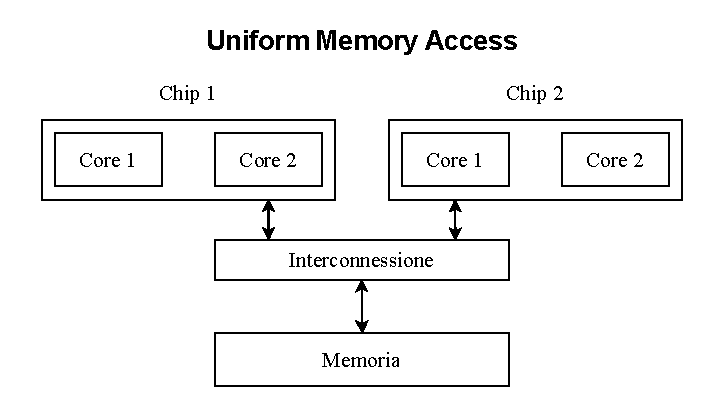
\includegraphics[width=0.7\textwidth ]{images/UMA.pdf}
\end{center}
In un sistema \textbf{UMA}, tutti i processori hanno accesso diretto alla memoria. Questo significa che qualsiasi processore può accedere a qualsiasi dato in memoria allo stesso tempo e con la stessa velocità, indipendentemente da dove si trovi fisicamente il dato.\begin{itemize}
    \item  I programmatori non devono preoccuparsi di gestire l'accesso alla memoria in modo complesso, poiché tutti i processori vedono la stessa memoria. 
    \item In molte applicazioni, l'accesso uniforme alla memoria può portare a prestazioni migliori, poiché i processori possono accedere ai dati di cui hanno bisogno rapidamente.
\end{itemize}
Differentemente, nei sistemi \textbf{NUMA}, i diversi core vengono partizionati in \textit{gruppi}, ed ogni gruppo dispone di una memoria principale distinta e disconnessa dalle altre, tale suddivisione è \textit{trasparente} al programmatore, in quanto funzionalmente la memoria viene vista come un unica unità.\begin{quote}
    I nodi sono interconnessi tra loro tramite un'interconnessione ad alta velocità, che consente ai processori di accedere alla memoria di altri nodi
\end{quote} Nonostante ciò, i core che accedono alla memoria del proprio gruppo saranno più rapidi rispetto quelli che accedono alla memoria di un gruppo diverso, per questioni di vicinanza fisica dei chip.\acc 
È possibile forzare l'allocazione della memoria su una specifica unità tramite l'inclusione della libreria \code{numa.h}.\begin{center}
    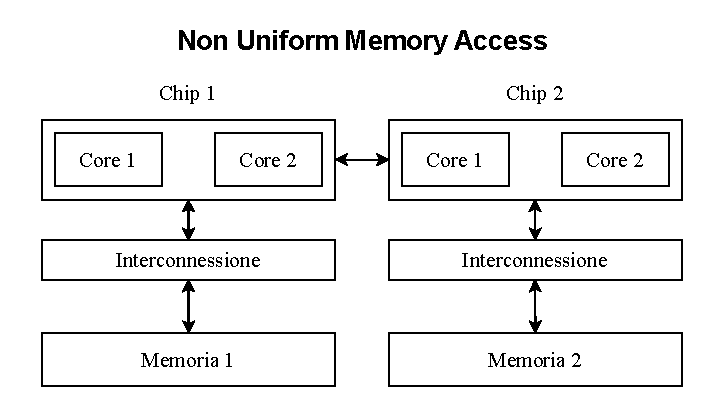
\includegraphics[width=0.7\textwidth ]{images/NUMA.pdf}
\end{center}
\chapter{Gestione dei Thread : OpenMP}
\textit{OpenMP} è un freamework di programmazione per i sistemi multicore a memoria condivisa, in particolare, costituisce un \textit{interfaccia} di gestione dei thread ad alto livello rispetto quella fornita da PThread. OpenMP vede il sistema come un'insieme di più CPU o core che possono accedere ad una memoria condivisa. In pratica, OpenMP permette di parallelizzare un codice sequenziale in maniera semplice tramite dei micro-interventi sul codice, tramite l'assistenza del compilatore.\acc 
Lo scopo di OpenMP è la decomposizione di alcune porzioni del programma al fine di renderle parallele (diramazione) per svolgere un determinato compito, alla fine di esso i thread possono essere eliminati ed il programma può tornare ad un esecuzione sequenziale.\begin{quote}
    il codice è globalmente sequenziale e localmente parallelo
\end{quote}
\begin{center}
    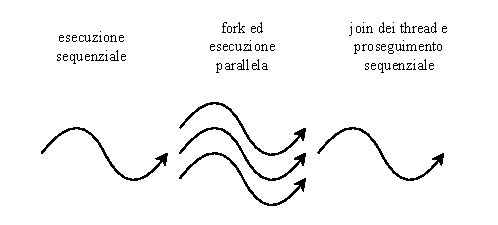
\includegraphics[width=0.7\textwidth ]{images/openMP.pdf}
\end{center}
Fa utilizzo di alcune direttive da dare al compilatore, per utilizzare OpenMP è quindi necessario sia importare la libreria \code{omp.h}, sia avere un compilatore che supporti le direttive, che in caso contrario verranno ignorate.
\section{Direttive pragma}
Le \textit{pragma} sono delle direttive speciali che elabora il pre processore, come anticipato, se openMP non è supportato dal compilatore, queste ultime verranno ignorate. Servono per conferire al sistema funzionalità non incluse nel comportamento standard del linguaggio C. \acc 
La direttiva più semplice ma anche più importante è\begin{quote}
    \code{\# pragma omp parallel}
\end{quote}
Una volta dichiarata nel codice, il blocco successivo verrà eseguito in parallelo (se e solo se il compilatore supporta OpenMP), è possibile sanche specificare il numero di thread che dovranno eseguire in parallelo il blocco. Sono anche fondamentali le seguenti funzioni 
\begin{itemize}
    \item \code{omp\_get\_thread\_num()} : ritorna l'identificatore del thread chiamante. 
    \item \code{omp\_get\_num\_threads()} : ritorna il numero di thread attivi. Se chiamata in una porzione sequenziale, ritornerà 1.
\end{itemize}
Si consideri il seguente esempio
\begin{lstlisting}[style=CStyle]
#include <stdio.h>
#include <stdlib.h> 
#include <omp.h>

void Hello (void);
int main(int argc, char** argv){
    int thread_count = atoi(argv[1]);
    #pragma omp parallel num_threads(thread_count)
    Hello(); /* verra' eseguita in parallelo */
    return 0;
}

void Hello(){
    int my_rank = omp_get_thread_num();
    int thread_count = omp_get_num_threads();
    printf("Hello from thread %d of %d",my_rank,thread_count);
}
\end{lstlisting}
La funzione \code{Hello()} essendo preceduta dalla direttiva pragma verrà eseguita in parallelo. OpenMP funziona come Pthreads, vi è un thread main che si occupa di eseguire i fork generando gli altri thread, per poi ri-congiungerli (join) ad una sola esecuzione. Per motivi di ottimizzazione, OpenMP potrebbe mantenere i thread sempre attivi in uno stato di "idle" (attesa), per poi richiamarli ed utilizzarli quando necessario, evitando di crearne di nuovi ogni volta.\acc 
\textbf{Attenzione} : Se OpenMP non è supportata la direttiva pragma sarà ignorata, però le funzioni \\\code{omp\_get\_thread\_num()}, \code{omp\_get\_num\_threads()} genereranno un errore di compilazione in quanto non sono definite. Quando si compila un codice che utilizza OpenMP va inclusa l'opzione 
\shell{-fopenmp}.\acc 
Il numero dei thread da eseguire può essere controllato in diversi modi\begin{itemize}
    \item È possibile impostare l'apposita variabile d'ambiente \code{OMP\_NUM\_THREADS} tramite la bash, ad esempio \begin{center}
        \shell{export OMP\_NUM\_THREADS=4}
    \end{center}
    Questa specifica varrà per tutti i programmi che faranno uso di OpenMP in quell'ambiente.
    \item Si può cambiare il numero di thread da eseguire tramite l'apposita funzione \code{omp\_set\_num\_threads()} all'interno del codice. 
    \item L'ultimo modo, mostrato nell'esempio superiore, è tramite la specifica nella direttiva pragma con la clausola \code{num\_threads}.
\end{itemize}
Come \code{num\_threads} esistono altre clausole in grado di modificare le direttive pragma, specificando dettagli aggiuntivi sul comportamento.\acc 
In base al sistema, potrebbero essere definite delle limitazioni riguardo il numero di thread che un programma può avviare, lo standard OpenMP non garantisce sempre che il numero di thread specificato nella clausola sia avviato, ma finché il numero di thread è ridotto, si può assumere che siano eseguiti quelli specificati. È importante sapere che al termine di ogni blocco parallelo vi è la presenza di una \textit{barriera} implicita.\acc 
L'insieme dei thread che vengono eseguiti in parallelo su uno stesso blocco è denominato \textit{team}, all'interno di esso si identificano
\begin{center}
	\begin{tabular}{>{\centering\arraybackslash}m{3in}>{\arraybackslash}m{3in}}
        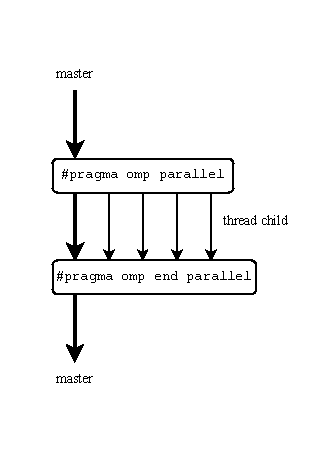
\includegraphics[width=0.4\textwidth ]{images/parallelConstruct.pdf} & \begin{itemize}
            \item \textbf{master} : il thread originale dell'esecuzione (che avvia la funzione \code{main()})
            \item \textbf{parent} : il thread che incontra la direttiva pragma sull'avvio dell'esecuzione in parallelo e si occupa di generare gli altri thread (spesso coincide con il master)
            \item \textbf{child} : ogni thread che viene avviato da un thread parent
        \end{itemize}
		\\
	\end{tabular}
\end{center}
Quando si include OpenMP nel proprio codice, si vuole far si che quest'ultimo sia flessibile anche nei sistemi il cui compilatore non supporta lo standard. Si è già accennato al fatto che le direttive pragma verranno ignorate in tal caso, non è però la stessa cosa per le funzioni di libreria come 
\code{omp\_set\_num\_threads()} o altre. È possibile utilizzare la variabile d'ambiente \code{\_OPENMP}, quest'ultima è definita nei sistemi che supportano OpenMP, quindi può essere argomento della direttiva \code{\#ifdef} in modo da rendere flessibile il codice permettendogli di evitare di chiamare funzioni di libreria che risulterebbero non dichiarate.
\begin{lstlisting}[style=CStyle]
#ifdef _OPENMP
    int my_rank = omp_get_thread_num();
    int thread_count = omp_get_num_threads();
#else 
    int my_rank = 0;
    int thread_count = 1;
#endif
\end{lstlisting}
\flowerLine
\section{Mutua Esclusione}
Nonostante OpenMP fornisca un interfacia di alto livello, è comunque possibile far cadere i thread in una situazione di race condition quando questi ultimi accedono a variabili condivise simultaneamente. A tal proposito, esiste una direttiva che permette di simulare una lock, in particolare, il blocco che segue la direttiva, si assume "chiuso" da una \code{lock} prima di esso, ed un \code{unlock} dopo. La direttiva in questione è\begin{quote}
    \code{\#pragma omp critical}
\end{quote}
Garantisce la mutua esclusione del blocco che segue.\acc 
Grazie alle direttive pragma è possibile trasformare un codice sequenziale in parallelo con l'aggiunto di pochissime linee di codice. Tale semplicità ha permesso ad OpenMP di essere adottato in moltissime applicazioni, ed essere utilizzato da coloro che non hanno una conoscienza approfondita dei sistemi multicore.
\subsection{Integrazione Numerica con OpenMP}
Il codice parallelizzato con OpenMP che esegue la regola del trapezoide per calcolare l'integrale definito di una funzione $f:\R\rightarrow \R$ è identico al sequenziale, ad eccetto dell'aggiunta di sole due linee di codice.
\begin{lstlisting}[style=CStyle]
#include <stdio.h>
#include <stdlib.h>
#include <opm.h>

void Trap(double a, double b, int n, double *global_result_p)
{
    double h, x, my_result;
    double local_a, local_b;
    int i, local_n;
    #ifdef _OPENMP
        int my_rank = omp_get_thread_num();
        int thread_count = omp_get_num_threads();
    #else
        int my_rank = 0;
        int thread_count = 1;
    #endif

    h = (b - a) / n;
    local_n = n / thread_count;
    local_a = a + my_rank * local_n * h;
    my_result = (f(local_a) + f(local_b)) / 2.0; /*f e' la funzione integranda*/
    for (i = 0; i <= local_n - 1; i++)
    {
        x = local_a + i * h;
        my_result += f(x);
    }
    my_result = my_result * h;
    #pragma omp critical
        *global_result_p += my_result;
}

void main(int argc, char **argv)
{
    double global_result = 0.0;
    double a, b;
    int n;
    int thread_count = atoi(argv[1]);
    printf("Enter a,b and n\n", &a, &b, &n);
    #pragma omp parallel num_threads(thread_count);
        Trap(a, b, n, &global_result);

    printf("result : %f", global_result);
}
\end{lstlisting}
Alcuni processore moderni implementano le operazioni di incremento come un unica istruzione atomica \begin{quote}
    \texttt{load + sum + store}
\end{quote}
In tal caso è possibile utilizzare la direttiva pragma \begin{quote}
    \code{\#pragma omp atomic}
\end{quote}
che risulta più efficiente della direttiva precedente in quanto copre la mutua esclusione solo dell'aggiornamento della variabile e non di tutto il blocco.\acc 
OpenMP è un interfaccia di alto livello che garantisce meno flessibilità e controllo rispetto PThread ma permette una parallelizzazione del codice più semplice, è inoltre portatile e può funzionare anche su Windows. Con OpenMP è possibile programmare la GPU.
\subsection{Riduzione}
OpenMP permette di eseguire le collettive di riduzione, come, ad esempio la chiamata \code{MPI\_Reduce}. Nell'esempio del trapezoide, ogni thread, piuttosto che restituire la somma parziale, si occupava di aggiornare la variabile condivisa, è possibile far si che i thread ritornino le somme parziali, e che queste ultime  vengano utilizzate in un'operazione di riduzione. \acc 
Le riduzioni in OpenMP sono operazioni binarie (come la somma o la moltiplicazione). 
È un calcolo che applica ripetutamente lo stesso operatore di riduzione a una sequenza di valori, fino a ottenere un unico risultato finale.
Tutti i risultati intermedi di questa operazione vengono accumulati in una stessa variabile, chiamata variabile di riduzione.\acc 
La clausola di riduzione viene aggiunta ad una direttiva pragma  ed è definita come segue \begin{quote}
    \code{reduction(<operator>:<variabile list>)}
\end{quote}
Bisogna specificare l'operatore da eseguire fra quelli disponibili 
\begin{lstlisting}[style=CStyle]
    +  *  -  &  |  ^  &&  ||
\end{lstlisting}
Va poi specificata la variabile in questione che conterrà il risultato finale
\begin{lstlisting}[style=CStyle]
global_result = 0.0;
#pragma omp parallel num_threads(thread_count) reduction(+:global_result)
    global_result += Local_trap(double a, double b, int n):
\end{lstlisting}
\flowerLine
\section{Scoping}
Con \textit{scope di una variabile}, si intendono le porzioni di codice in cui quella variabile è accessibile e può essere utilizzata, definisce il ciclo di vita/visibilità delle variabili. Nei programmi paralleli con OpenMP, con scope ci si riferisce all'insieme di thread che può accedere la specifica variabile nel blocco parallelo. Una variabile può essere\begin{itemize}
    \item \textbf{shared} : accessibile da ogni thread del blocco. Le variabili dichiarate prima di un blocco parallelo rientrano in questa categoria. Inoltre anche le zone di memoria allocate sullo stack del thread master sono accessibili dai suoi figli.
    \item \textbf{private} : accessibile da un singolo thread, le variabili dichiarate all'interno di un blocco parallelo sono private, ed ogni thread ne avrà una sua copia distinta dalle altre.
\end{itemize}
È possibile specificare la visibilità di ogni singola variabile tramite delle clausole apposite, con la clausola \begin{quote}
    \code{default(none)}
\end{quote}
si sta dicendo al compilatore che, per default, nessuna variabile dichiarata al di fuori del blocco sarà considerata automaticamente privata o condivisa all'interno di quel blocco. Ciò significa che il programmatore dovrà specificare esplicitamente lo scope di ogni variabile che vuole utilizzare, evitando ambiguità. Data una variabile, le clausole di specifica disponibili sono le seguenti\begin{itemize}
    \item \code{shared} : è il comportamento di default delle variabili al di fuori del blocco parallelo, va quindi specificata per queste ultime solo se presente anche la clausola \code{default(none)}
    \item \code{reduction} : si specifica che una variabile dovrà essere soggetta ad un operazione di riduzione. Ci saranno delle copie di quest'ultima private per ogni thread, ma il risultato finale sarà condiviso
    \item \code{private} : la variabile avrà una copia privata per ogni thread nel blocco. Le variabili private \underline{non sono inizializzate}.
\end{itemize}
\begin{lstlisting}[style=CStyle]
int x = 5;
#pragma omp parallel private(x)
    {
        x= x + 1;
    }
printf("x is %d", x);
\end{lstlisting}
Nel blocco di codice mostrato, la chiamata di funzione \texttt{printf} stamperà in output \texttt{"x is 5"}. Inoltre, l'incremento di \texttt{x} all'interno del blocco parallelo può causare errore in quanto \texttt{x} è privata e non inizializzata.\acc 
Esistono altre 4 clausole per specificare lo scope di una variabile\begin{itemize}
    \item \code{firstprivate} : Come la clausola \code{private}, crea una copia locale della variabile per ogni thread all'interno del blocco parallelo.
    A differenza di \code{private}, la copia locale viene inizializzata con il valore della variabile originale (quella "esterna" al blocco) prima che il blocco venga eseguito.
    \item \code{lastprivate} : Anche questa clausola crea copie locali delle variabili, come \code{private}.
    Al termine dell'esecuzione del blocco parallelo, il valore della copia locale dell'ultimo thread che ha completato il ciclo viene copiato nella variabile originale (quella "esterna" al blocco).
\end{itemize}
Quando dichiariamo una variabile come \code{private} in un contesto di programmazione parallela, questa diventa inaccessibile al di fuori del blocco di codice in cui è stata dichiarata. Questo è utile per evitare conflitti tra i thread, ma a volte può essere necessario avere una variabile privata che persista tra diverse sezioni parallele.
\begin{itemize}
\item \code{threadprivate} : Crea una copia locale e persistente di una variabile globale o statica per ogni thread. Questa copia è accessibile solo al thread corrispondente e mantiene il suo valore per tutta la durata del programma. È ideale quando è necessario conservare dati privati che devono essere mantenuti tra diverse sezioni parallele, ma che non devono essere condivisi tra i thread.
\item \code{copyin} : Viene utilizzata in combinazione con \code{threadprivate} per inizializzare le copie locali di ogni thread con il valore della variabile originale (quella definita nel thread master).
È utile quando si vuole che tutti i thread inizino con lo stesso valore iniziale per una variabile privata persistente.
\end{itemize}
\subsubsection{Esempio riassuntivo}
\begin{lstlisting}[style=CStyle]
#include <omp.h>
int x, y, z[1000];
#pragma omp threadprivate(x)

void default_none(int a){
    const int c = 1;
    int i = 0;
    #pragma omp parallel default(none) private(a) shared(z)
    {
        int j = omp_get_num_threads();
        a = z[j]; /* OK : 'j' e' dichiarata nella sezione parallela */
        x = c; /* OK : 'x' e' threadprivate */
        z[i] = y; /* Errore : non si possono referenziare 'i' o 'y', data 
                     la clausola default(none) */
    }
}
\end{lstlisting}
\flowerLine 
\section{Cicli For Paralleli}
Si vogliono parallelizzare le iterazioni (indipendenti) dei blocchi ciclici nel C, queste ultime sono spesso le operazioni più dispendiose, rendendo favorevole una loro parallelizzazione. OpenMP è in grado di parallelizzare esclusivamente i cicli \code{for}, è assolutamente necessario che il numero di iterazioni totali sia noto a priori. La direttiva \begin{quote}
    \code{\#pragma omp parallel for}
\end{quote}
permette di parallelizzare un ciclo for, facendo si che ogni thread si occuperà di un sottoinsieme delle iterazioni totali. Un ciclo for per essere parallelizzato deve avere la seguente struttura 
$$ \texttt{for}\begin{pmatrix}
    &&\texttt{index++}\\ 
    &&\texttt{++index}\\ 
    &\texttt{index<end;}&\texttt{index--}\\ 
    &\texttt{index<=end;}&\texttt{--index}\\ 
    \texttt{index=start;}&\texttt{index>=end;}&\texttt{index+=incr}\\ 
    &\texttt{index>end;}&\texttt{index=incr+index}\\ 
    &&\texttt{index-=incr}\\ 
    &&\texttt{index=index+incr}\\
    &&\texttt{index=index-incr}
\end{pmatrix}$$
solo in questo modo il numero di iterazioni sarà noto a priori. È quindi importante che\begin{itemize}
    \item la variabile \code{index} sia un tipo intero o puntatore. 
    \item \code{start},\code{end},\code{incr} devono avere tipi compatibili. 
    \item \code{incr} deve essere costante. 
    \item l'indice del ciclo \code{index} non può essere modificato all'interno del ciclo, ma solo tramite l'espressione di incremento.
\end{itemize} Il seguente codice riporta un esempio di for paralellizzato nell'ambito dell'integrazione con la regola del trapezoide.
\begin{lstlisting}[style=CStyle]
h=(b-a)/n;
approx=(f(a)+f(b))/2.;
#pragma omp parallel for num_threads(thread_count) reduction(+:approx)
for(int i = 1;i<n;i++){
    approx+=f(a+i*h);
}
approx=h*approx;
\end{lstlisting}
Il seguente ciclo 
\begin{lstlisting}[style=CStyle]
for(i=0;i<n;i++){
    if([condizione])
        break;
}
\end{lstlisting}
non può essere parallelizzato perché il numero di iterazioni non è noto a priori. Anche il seguente
\begin{lstlisting}[style=CStyle]
for(i=0;i<n;i++){
    if([condizione])
        i++;
}
\end{lstlisting}
non può essere parallelizzato perché l'indice viene incrementato dentro il ciclo. Il seguente 
\begin{lstlisting}[style=CStyle]
for(i=0;i<n;i++){
    if([condizione])
        exit();
}
\end{lstlisting}
nonostante il numero di iterazioni non sia noto a priori, può essere parallelizzato perché la clausola \code{exit()} termina l'intero programma e non è quindi necessario preoccuparsi di un eventuale comportamento anomalo.
\subsection{Cicli Annidati}
Nella maggior parte dei casi in cui ci sono due cicli for annidati, è sufficiente parallelizzare solo il primo ciclo. È importante sapere che alla fine di ogni ciclo for parallelizzato è presente una \textit{barriera implicita}. Il seguente esempio mostra come vengono suddivise le iterazioni ai vari thread in un ciclo for parallelizzato.
\begin{lstlisting}[style=CStyle]
#pragma omp parallel for num_threads(thread_count) 
for(i=0;i<4;i++){
    for(i=0;i<4;i++){
        c(i,j);
    }
}
\end{lstlisting}
\begin{center}
    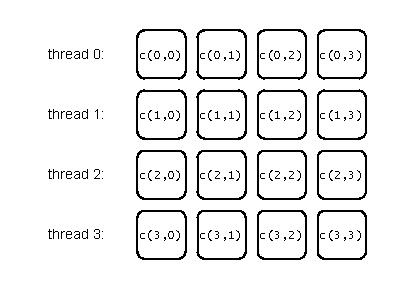
\includegraphics[width=0.5\textwidth ]{images/cicliAnnidati.drawio.pdf}
\end{center}
Ogni thread (dei 4) esegue una iterazione del ciclo for esterno (parallelizzato), e per ognuna di questa, esegue le 4 iterazioni del ciclo for interno non parallelizzato. Si consideri la seguente situazione, in cui ci sono 4 thread, ed un ciclo esterno di 3 iterazioni.
\begin{lstlisting}[style=CStyle]
#pragma omp parallel for num_threads(thread_count) 
for(i=0;i<3;i++){
    for(i=0;i<6;i++){
        c(i,j);
    }
}
\end{lstlisting}
le iterazioni sono assegnate in questo modo
    \begin{center}
        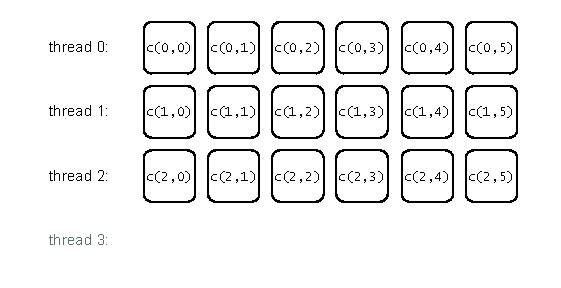
\includegraphics[width=0.6\textwidth ]{images/cicliAnnidati2.drawio.pdf}
    \end{center}
I 3 cicli esterni verranno assegnati ai primi 3 thread, il quarto thread quindi non verrà considerato nel calcolo parallelo, in tal modo la distribuzione del carico di lavoro è poco uniforme e certamente non efficiente. È sicuramente meglio parallelizzare il for interno\begin{itemize}
    \item ad ogni iterazione esterna, il ciclo interno (di 6 iterazioni) eseguito da 4 thread \item i primi due thread eseguiranno 2 iterazioni, gli altri due 1 iterazione.
\end{itemize}
\begin{lstlisting}[style=CStyle]
for(i=0;i<3;i++){
#pragma omp parallel for num_threads(thread_count) 
    for(i=0;i<6;i++){
        c(i,j);
    }
}
\end{lstlisting}
\begin{center}
    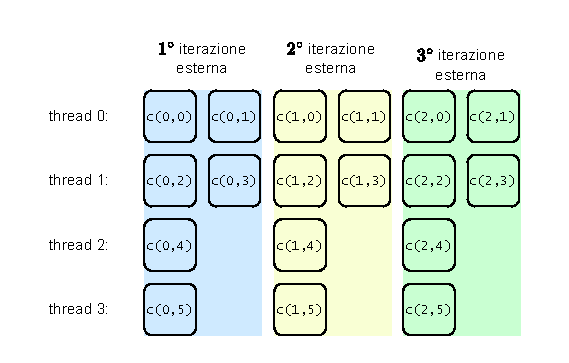
\includegraphics[width=0.6\textwidth ]{images/cicliAnnidati3.drawio.pdf}
\end{center}
Nonostante questa soluzione sia migliore della precedente, non è ancora ottimale. La soluzione migliore (nei casi in cui i cicli annidati sono molto semplici) è di collassare i due cicli in un unico ciclo tramite degli accorgimenti sugli indici, ad esempio:
\begin{lstlisting}[style=CStyle]
#pragma omp parallel for num_threads(thread_count) 
for(ij=0;ij<3*6;ij++){
    c(ij/6, ij%6);
}
\end{lstlisting}
In questo caso la distribuzione dei cicli è ottimale (il più uniforme possibile).
\begin{center}
    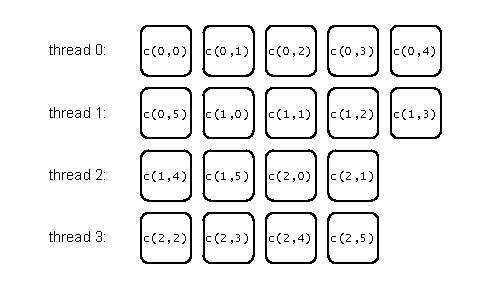
\includegraphics[width=0.6\textwidth ]{images/cicliAnnidati4.pdf}
\end{center}
OpenMP fornisce una clausola per collassare automaticamente due cicli for annidati in uno singolo, ossia  
\begin{quote}
    \code{collapse(f)}
\end{quote}
Dove \code{f} è il numero di cicli da collassare. Risulta piuttosto utile nei casi come il precedente, quando il numero di iterazioni del ciclo esterno è basso (paragonabile, se non minore, dei core sulla macchina).
\begin{lstlisting}[style=CStyle]
#pragma omp parallel for num_threads(thread_count) collapse(2)
for(i=0;i<3;i++){
    for(i=0;i<6;i++){
        c(i,j);
    }
}
\end{lstlisting}
Di default, è vietato parallelizzare due cicli annidati con la direttiva \code{parallel for}.
\begin{lstlisting}[style=CStyle]
#pragma omp parallel for num_threads(thread_count) 
for(i=0;i<3;i++){
    #pragma omp parallel for num_threads(thread_count)  /* VIETATO */
    for(i=0;i<6;i++){
        c(i,j);
    }
}
\end{lstlisting}
\subsection{Iterazioni Dipendenti}
La parallelizzazione di un ciclo for non impone alcun ordinamento sulle iterazioni, è possibile che un thread esegua l'iterazione \texttt{i+1} prima di un thread che esegue la \texttt{i}, è quindi ovvio che è possibile parallelizzare un ciclo finché le iterazioni sono indipendenti fra loro.\acc 
Il seguente esempio è il più esplicativo, per calcolare l'$i$-esimo numero di fibonacci è necessario conoscerne l'$i-1$-esimo, non è quindi assicurata la correttezza di un ciclo parallelizzato che deve calcolare la sequenza dei primi $n$ numeri di fibonacci.
\begin{lstlisting}[style=CStyle]
fibo[0]= fibo[1]=1;
#pragma omp parallel for num_threads(thread_count) 
for(i=2;i<n;i++){
    fibo[i]= fibo[i-1] + fibo[i-2];
}
\end{lstlisting}
Perché non funziona? \begin{itemize}
   \item l'iterazione \texttt{i=3} potrebbe essere calcolata prima dell'iterazione \texttt{i=2}, supponiamo sia questo il caso 
   \item l'iterazione \texttt{i=3} considerà l'elemento \texttt{fibo[2]}, questo dovrebbe essere uguale a 2, ma visto che l'iterazione \texttt{i=2} non è stata eseguita, il valore dentro l'array è nullo, 
   \item l'iterazione \texttt{i=3} calcolerà \code{fibo[3]=fibo[2]+fibo[1]=0+1=1} 
   \item il risultato è sbagliato in quanto il terzo numero di fibonacci è 3.
\end{itemize}
Quando si parallelizza un ciclo for è obbligatorio assicurarsi che non ci siano dipendenze fra i dati tra le varie iterazioni, dipendenze di questo tipo sono dette \textbf{loop-carried dependence}. Bisogna modificare il codice dei cicli per rendere le iterazioni indipendenti.\acc 
Dato un loop della seguente forma
\begin{lstlisting}[style=CStyle]
for(i=...){
    ... 
    S1 : operazione sulla locazione di memoria x
    ... 
    S2 : operazione sulla locazione di memoria x
    ...
}
\end{lstlisting}
ci sono due operazioni su una stessa locazione di memoria, essendo queste contenute in un unica iterazione, si ha la certezza che verranno eseguite da uno stesso thread nell'ordine in cui sono state stabilite. Il problema si verifica quando due operazioni che vanno eseguite sequenzialmente, si trovano in due iterazioni differenti, ad esempio
\begin{lstlisting}[style=CStyle]
for(i=...){
    ... 
    S2 : operazione sul valore x[i-1]
    ... 
    S1 : operazione sul valore x[i]
    ...
}
\end{lstlisting}
in questo caso l'operazione \texttt{S2} potrebbe essere eseguita prima dell'operazione \texttt{S1} se un'iterazione \texttt{i} viene eseguite prima dell'iterazione \texttt{i-1}. \acc 
Ci sono 4 differenti tipi di dipendenze che coinvolgono due operazioni \texttt{S1},\texttt{S2} che non possono essere eseguite in due iterazioni differenti:\begin{itemize}
    \item \textbf{RAW} : Read After Write (una lettura dopo una scrittura)
\begin{lstlisting}[style=CStyle]
x=10;       //S1
y=2*x+5;    //S2
\end{lstlisting}
    se \texttt{S2} fosse eseguita per prima, potrebbe leggere un valore di \texttt{x} non corretto.
    \item \textbf{WAR} : Write After Read (una scrittura dopo una lettura)
\begin{lstlisting}[style=CStyle]
y=x+3;       //S1
x++;         //S2
\end{lstlisting}
    se \texttt{S2} fosse eseguita per prima, la variabile \texttt{y} leggerebbe un valore errato di \texttt{x}.
    \item \textbf{WAW} : Write After Write (una scrittura dopo una scrittura)
\begin{lstlisting}[style=CStyle]
x=10;       //S1
x=x+c;      //S2
\end{lstlisting}
        se \texttt{S2} fosse eseguita per prima, verrebbe incrementata anche se \texttt{x} dovesse essere diverso da 10, anche se ogni volta che si esegue \texttt{S2}, dovrebbe sempre essere uguale a 10.
    \item \textbf{RAR} : Read After Read (una lettura dopo una lettura)
\begin{lstlisting}[style=CStyle]
y=x+c;      //S1
z=2*x+1;    //S2
\end{lstlisting}
non è una vera dipendenza e non causa problemi.
\end{itemize}
\subsection{Risoluzione delle Dipendenze RAW}
In \textit{alcuni casi} è possibile rimuovere le dipendenze di tipo RAW nei cicli, in particolare, si identificano 6 metodologie di risoluzione. 
\subsubsection{1) Sistemare le induction/reduction variable}
Si consideri il seguente ciclo:
\begin{lstlisting}[style=CStyle]
double v = start;
double sum = 0;
for(int i = 0; i < N; i++){
    sum = sum + f(v);   //S1
    v = v + step;       //S2
}
\end{lstlisting}
\defi{} Una \textit{induction variable}, o \textit{variabile induttiva}, è una variabile che all'interno di un ciclo viene incrementata di un valore costante ad ogni iterazione.\acc 
Le dipendenze sono\begin{itemize}
    \item una dipendenza di tipo RAW per l'operazione \texttt{S1} sulla variabile di riduzione \texttt{sum}, che ad ogni iterazione, utilizza il valore dell'iterazione precedente. 
    \item una dipendenza di tipo RAW per l'operazione \texttt{S2} sulla variabile induttiva \texttt{v}, che ad ogni iterazione, utilizza il valore dell'iterazione precedente. 
    \item una dipendenza di tipo RAW fra le due operazioni, dato che \texttt{S1} utilizza il valore di \texttt{v} calcolato all'iterazione precedente.
\end{itemize}
Essendo che \texttt{v} è una variabile induttiva, il suo valore può essere calcolato a prescindere per ogni iterazione \texttt{i} in maniera indipendente.\begin{quote}
    \code{i = 0} $ \ \implies \ $ \code{v = start}\\ 
    \code{i = 1} $ \ \implies \ $ \code{v = start + step}\\ 
    \code{i = 2} $ \ \implies \ $ \code{v = (start + step) + step}\\ 
    $\vdots$ \\ 
    \code{i = k} $ \ \implies \ $ \code{v = start + step*k}\\ 
\end{quote}
è quindi possibile rimuovere due dipendenze calcolando \code{v} a partire dall'indice \texttt{i} senza dover utilizzare il valore dell'iterazione precedente.
\begin{lstlisting}[style=CStyle]
double v = start;
double sum = 0;
for(int i = 0; i < N; i++){
    v = start + i*step;       
    sum = sum + f(v);   
}
\end{lstlisting}
L'unica dipendenza da risolvere riguarda il valore di \code{sum} che è dipendente dalle precedenti iterazioni, ma per ovviare a ciò, è sufficiente specificare che \code{sum} è una variabile di riduzione nella direttiva pragma, facendo si che se ne occupi openMP.
\begin{lstlisting}[style=CStyle]
double v = start;
double sum = 0;
#pragma omp parallel for reduction(+:sum) private(v)
for(int i = 0; i < N; i++){
    v = start + i*step;       
    sum = sum + f(v);   
}
\end{lstlisting}
\subsubsection{2) Loop skewing}
Questa tecnica consiste nel riarrangiare il loop eseguendo una sottospecie di "shift" delle operazioni (l'esempio renderà chiaro il concetto). Si consideri la seguente porzione di codice:
\begin{lstlisting}[style=CStyle]
for(int i = 1; i < N; i++){
    y[i]= f(x[i-1]);
    x[i]=x[i]+c[i];
}
\end{lstlisting}
Il ciclo \texttt{i} è dipendente dal ciclo \texttt{i-1}, in quanto \code{y[i]} per essere aggiornata necessita di \code{x[i-1]}. In questo metodo, si "srotola" il loop, considerando le diverse iterazioni in sequenza, ad esempio:
\begin{center}
    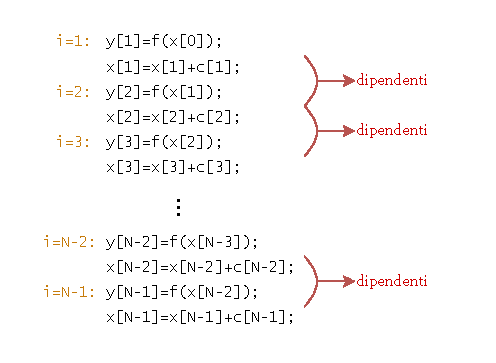
\includegraphics[width=0.6\textwidth ]{images/skewing.pdf}
\end{center}
Basta raggruppare in un'unica iterazione le operazioni dipendenti, "shiftando" di un operazione il ciclo for, come segue
\begin{lstlisting}[style=CStyle]
y[1]=f(x[0]);
for(int i = 1; i < N-1; i++){
    x[i]=x[i]+c[i];
    y[i+1]= f(x[i]);
}
x[N-1]=x[N-1]+c[N-1];
\end{lstlisting}
Riscrivendo il ciclo in questo modo si sono rimosse le dipendenze fra diverse iterazioni, ed il ciclo può essere parallelizzato.
\subsubsection{3) Parallelizzazione parziale}
Questa metodologia è la più semplice, consiste nell'individuare le iterazioni indipendenti tramite la costruzione di un grafo., si consideri il seguente ciclo annidato 
\begin{lstlisting}[style=CStyle]
for(int i = 1; i < N; i++){
    for(int j = 1; j < M; j++){
        data[i][j]=data[i-1][j]+data[i-1][j-1];
    }
}
\end{lstlisting}
si disegna un grafo in cui ogni nodo rappresenta un iterazione, e vi è un arco dal nodo $q$ al nodo $q'$ se l'iterazione $q'$ è dipendente dal nodo $q$. Nell'esempio del ciclo riportato qua sopra, si ha il seguente grafo:\begin{center}
    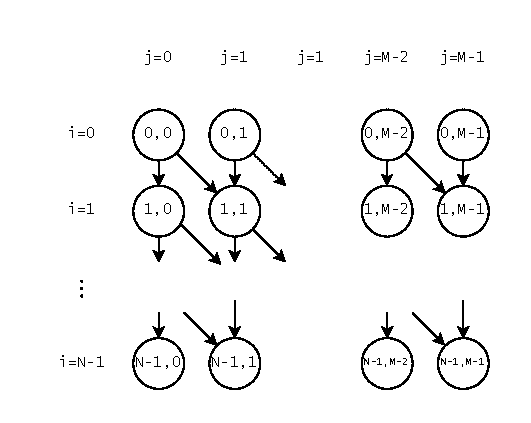
\includegraphics[width=0.6\textwidth ]{images/grafoIterazioni.drawio.pdf}
\end{center}
Si osserva che non ci sono archi che collegano due nodi sulla stessa riga, quindi le righe possono essere parallelizzate senza problemi, in quanto le iterazioni su ogni riga (ossia, fissato \texttt{i} e al variare di \texttt{j}) non sono dipendenti fra loro.
\begin{lstlisting}[style=CStyle]
for(int i = 1; i < N; i++){
    #pragma omp parallel for 
    for(int j = 1; j < M; j++){
        data[i][j]=data[i-1][j]+data[i-1][j-1];
    }
}
\end{lstlisting}
Anche se apparentemente l'iterazione \code{j} dipende dall'iterazione \code{j-1}, si ha che \code{j} è eseguita all'iterazione esterna \code{i}, e  \code{j-1} è eseguita all'iterazione esterna \code{i-1}, essendo garantita la sequenzialità dell'ordinamento esterno, questa dipendenza apparente su \code{j} non causa problemi.
\subsubsection{4) Refactoring} 
Questo metodo consiste nella riscrittura dei cicli in modo da renderli parallelizzabili, si consideri il seguente esempio
\begin{lstlisting}[style=CStyle]
for(int i = 1; i < N; i++){
    for(int j = 1; j < M; j++){
        data[i][j]=data[i-1][j]+data[i-1][j-1]+data[i][j-1];
    }
}
\end{lstlisting}
si ha il seguente grafo:\begin{center}
    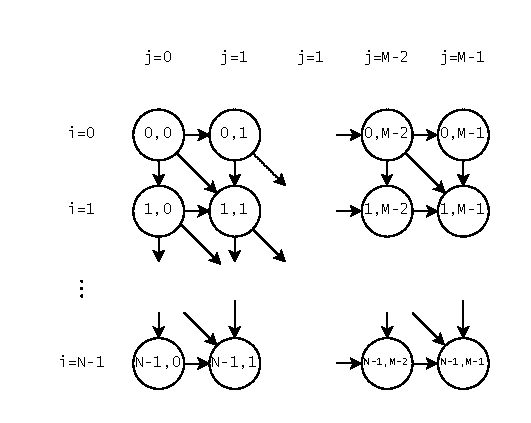
\includegraphics[width=0.5\textwidth ]{images/grafoIterazioni2.drawio.pdf}
\end{center}
In questo caso anche le righe sono dipendenti fra loro, ed il ciclo sembra non parallelizzabile. Che succede se si considerano i nodi sulle diagonali del grafo?
\begin{center}
    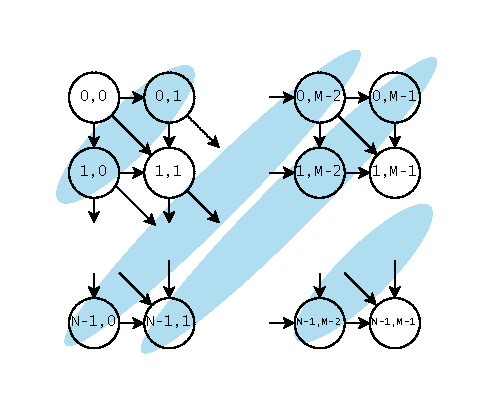
\includegraphics[width=0.5\textwidth ]{images/grafoIterazioni3.drawio.pdf}
\end{center}
non ci sono dipendenze fra le iterazioni sulla diagonale, queste si definiscono \textit{onde}, e possono essere parallelizzate, anche se è difficile individuarle nel codice, ed il ciclo va completamente riscritto. Un idea di implementazione può essere la seguente:
\begin{lstlisting}[style=CStyle]
for(wave = 0; wave<NumWaves; wave++){
    diag=F(wave);
    #pragma omp parallel for 
    for(k=0; k < diag; k++){
        int i = get_i(diag,k);
        int j = get_j(diag,k);
        data[i][j]=data[i-1][j]+data[i-1][j-1]+data[i][j-1];
    }
}
\end{lstlisting}
\subsubsection{5) Fissione del Loop} 
Si divide semplicemente il loop in una parte parallelizzabile ed in una parte sequenziale. Il ciclo
\begin{lstlisting}[style=CStyle]
s=b[0];
for(int i = 1;i < N;i++){
    a[i]=a[i]+a[i-1]; //S1
    s=s+b[i];         //S2
}
\end{lstlisting}
ha l'operazione \texttt{S1} che non si può parallelizzare, e l'operazione \texttt{S2} che può essere parallelizzata, quindi si divide in due cicli:
\begin{lstlisting}[style=CStyle]
for(int i = 1;i < N;i++){
    a[i]=a[i]+a[i-1]; //S1
}
s=b[0];
#pragma omp parallel for 
for(int i = 1;i < N;i++){
    s=s+b[i];         //S2
}
\end{lstlisting}
\subsubsection{6) Cambio dell'algoritmo}
Se nessun metodo precedente è applicabile, è necessario cambiare totalmente l'algoritmo, ad esempio, la sequenza di fibonacci può essere parallelizzata se calcolata tramite la formula di Binet: 
$$F_n=\frac{\varphi^n-(1-\varphi)^n}{\sqrt{5}} $$ 
\begin{lstlisting}[style=CStyle]
fibo[0]=fibo[1]=1;
#pragma omp parallel for 
for(int i=2;i < N;i++){
    fibo[i]=(exp(phi,n)-exp(1-phi,n))/sqrt(5);
}
\end{lstlisting}
\subsection{Rimozione di dipendenze WAR e WAW}
Le dipendenze WAR possono essere risolte semplicemente, si consideri il seguente ciclo
\begin{lstlisting}[style=CStyle]
for(int i=0;i < N-1;i++){
    a[i]=a[i+1]+c;
}
\end{lstlisting}
Nell'iterazione \code{i} si scrive un valore che verrà letto nell'iterazione successiva \code{i+1}. È sufficiente creare una copia dell'array \code{a[]} da utilizzare nel ciclo da parallelizzare.
\begin{lstlisting}[style=CStyle]
for(int i=0;i < N-1;i++){
    a2[i]=a[i+1];
}

#pragma omp parallel for 
for(int i=0;i < N-1;i++){
    a[i]=a2[i]+c;
}
\end{lstlisting}
Bisogna valutare se il tempo risparmiato nel parallelizzare il ciclo sia minore o maggiore del tempo utilizzato per eseguire la copia dell'array.\acc 
Anche le dipendenze WAW possono essere risolte, spesso è sufficiente usare un costrutto di openMP, si consideri il seguente ciclo
\begin{lstlisting}[style=CStyle]
for(int i = 0; i < N; i++){
    y[i]=a*x[i]+c;  //S1 
    d=fabs(y[i]);   //S2
}
\end{lstlisting}
la dipendenza è sulla variabile \texttt{d}, il valore finale di questa, una volta che termina la sezione  parallela, deve essere quello calcolato nell'ultima iterazione, ossia \code{fabs(y[N-1])}. È sufficiente utilizzare la clausole \code{lastprivate} per propagare all'esterno del for il valore di \texttt{d} calcolato dal thread che ha eseguito l'ultima iterazione.
\begin{lstlisting}[style=CStyle]
#pragma omp parallel for shared(a, c) lastprivate(d)
for(int i = 0; i < N; i++){
    y[i]=a*x[i]+c;  //S1 
    d=fabs(y[i]);   //S2
}
\end{lstlisting}

\end{document}